\documentclass[runningheads]{llncs}

\usepackage[T1]{fontenc}
\usepackage{graphicx}
\usepackage{amsmath,amssymb}
\usepackage{booktabs}
\usepackage{array}
\usepackage{rotating}
\usepackage{microtype}
\usepackage{tikz}
\usetikzlibrary{arrows.meta,positioning}
\usepackage[hidelinks]{hyperref}
\usepackage{xurl}

\graphicspath{{figures/}}
\newcommand{\GER}{\mathrm{GER}}

\begin{document}

\title{Modelling State-Level Gross Enrolment Ratio in Indian Higher Education: Correlates, Validation and a 2035 Projection}
\titlerunning{Modelling State-Level GER in Indian Higher Education}

\author{Himanshu Kumar Jha\inst{1}}
\authorrunning{H. K. Jha}

\institute{Department of Computer Science, Ramanujan College, University of Delhi, New Delhi, India\\
\email{himanshu.jha013@gmail.com}}

\maketitle

\begin{abstract}
India's National Education Policy 2020 targets a 50\% Gross Enrolment Ratio (GER) in higher education by 2035, up from 28.4\% in 2021-22. National averages conceal wide State disparities, with populous States furthest behind. This study asks how strongly State GER is associated with college density, pupil--teacher ratio (PTR) and Gender Parity Index (GPI, female GER divided by male GER); whether these associations survive out-of-sample and panel checks; and what recent trends imply for 2035-36. Using Open Government Data for 2021-22 and All India Survey on Higher Education predictors across 28 States, we compare a mean baseline against five learned models under leave-one-out cross-validation (LOOCV) and repeated five-fold cross-validation. Ordinary least squares yields an in-sample $R^2$ of 0.543 and LOOCV $R^2$ of 0.370 (LOOCV RMSE 6.86 vs.\ 8.97 GER points for the baseline). College density is the only robust correlate: each additional college per lakh 18--23 population corresponds to $+0.353$ GER points (95\% bootstrap interval 0.11 to 0.66), surviving State fixed effects and first differences. Under recent trends, 13 of 28 States reach 50\% by 2035-36, yet population-weighted GER reaches only 43.5\%, leaving 68.6\% of the youth cohort in off-track States.

\keywords{Gross Enrolment Ratio \and Indian higher education \and NEP 2020 \and college density \and leave-one-out cross-validation \and panel data \and SDG 4}
\end{abstract}

\section{Introduction}

\subsection{Policy context}

India operates one of the largest higher-education systems in the world, yet participation remains low relative to the size of its youth cohort. The National Education Policy 2020 sets a target of 50\% GER in higher education, including vocational education, by 2035 \cite{nep2020}. The official all-India GER was 28.4\% in 2021-22, an improvement of about one percentage point over 2020-21 but still roughly 22 points short of the goal \cite{aishe2023,ogd2025}. The Covid-19 period disrupted both enrolment and the administrative data series, so the recent trend is an uncertain guide to the next fourteen years.

The primary users of this analysis are State higher-education departments, which decide where to sanction new colleges and how to allocate faculty, and the central NEP monitoring cell, which tracks whether the 50\% target is reachable. The decision is not whether to expand---the target already commits the system to expansion---but where additional capacity would raise participation most per rupee. The question also sits within the international Sustainable Development Goal (SDG) 4 framework: target 4.3 commits governments to equal access for all women and men to affordable, quality technical, vocational and tertiary education by 2030 \cite{unesco2020}. According to the same UNESCO monitoring report, global tertiary GER reached 39\% (growing by roughly one percentage point per year since 2000), placing India's 28.4\% over ten points below the global benchmark, while participation in low- and middle-income countries remains heavily concentrated among the richest households \cite{unesco2020}. India's State-level gap is therefore both a national policy problem and part of the wider SDG 4 agenda.

The national figure is an average over units with very different starting points. In 2021-22, State GER ranged from 16.9\% in Assam to 47.0\% in Tamil Nadu; among Union Territories, Chandigarh reported 64.8\% and Dadra and Nagar Haveli and Daman and Diu 11.2\%. Fourteen of the 28 States were below 30\%, and none of the States had reached 50\%. Because education is on the concurrent list and because the demographic weight sits in the low-GER States, the national target is effectively a problem of State-level convergence.

\subsection{Research questions}

The project addresses three questions.

\begin{enumerate}
  \item \textbf{Association.} Conditional on the other indicators, how much independent information do college density, PTR and gender parity carry about State GER?
  \item \textbf{Stability.} Do those associations survive out-of-sample prediction, influence diagnostics and within-State panel variation, or are they artefacts of a 28-unit cross-section?
  \item \textbf{Projection.} Under explicit and auditable assumptions about density expansion, teacher supply and the common participation trend, which States reach 50\% by 2035-36, and what does that imply for the national target?
\end{enumerate}

The design is deliberately modest about causality. A cross-section of 28 States cannot identify the causal effect of building a college. It can, however, quantify conditional associations, test their fragility, and show how much the 2035 answer depends on assumptions that are usually left implicit.

\subsection{Contributions}

The study makes five methodological and reproducibility contributions.

\begin{itemize}
  \item It constructs an auditable, India-specific dataset from official government sources, cross-checked against published AISHE tables and stored with SHA-256 checksums and an explicit missingness audit.
  \item It implements a leakage-free nested cross-validation protocol across linear, regularised and non-parametric learners, and demonstrates why a better-fitting polynomial specification must be rejected for out-of-range extrapolation.
  \item It pairs point estimates with HC3 standard errors, 2,000-resample bootstrap intervals, variance inflation factors, residual specification tests, skewness/log-transform checks and leave-one-out influence analysis.
  \item It tests cross-sectional patterns against five-year within-State panel specifications and documents why the sign reversal on PTR serves as a cautionary negative finding.
  \item It provides a transparent, change-based projection framework with Monte Carlo uncertainty propagation and population-weighted aggregation to contrast State counts against cohort coverage.
\end{itemize}

Section~\ref{sec:related} reviews related work. Section~\ref{sec:data} describes the data and preprocessing, Section~\ref{sec:methods} the methods, Section~\ref{sec:setup} the experimental setup, Section~\ref{sec:results} the results, Section~\ref{sec:discussion} the discussion, and Section~\ref{sec:limitations} the limitations. Section~\ref{sec:conclusion} concludes.

\section{Related Work}\label{sec:related}

\subsection{Determinants of higher-education participation}

The literature on Indian higher education groups the determinants of participation into demand-side and supply-side factors. Demand-side accounts emphasise household income, secondary completion, aspirations, caste and gender norms, and the expected return to a degree \cite{sharma2026,ghosh2021}. Supply-side accounts emphasise the number and location of institutions, the availability of teachers, programme mix, distance education and affirmative-action capacity. Recent State-level work reaches similar conclusions. Sharma et al.~\cite{sharma2026} show that private provision narrows regional GER gaps but not socio-economic gaps; Kadlak and Behera~\cite{kadlak2026} argue that the aggregate GER masks district-level access in Maharashtra; Mitra and Ghara~\cite{mitra2019} document district-level variation within West Bengal; and Baruah and Goswami~\cite{baruah2024} evaluate the effect of the Rashtriya Uchchatar Shiksha Abhiyan on GER. Ghosh and Kundu~\cite{ghosh2021} find that women's participation varies sharply across major States. Outside India, Akinola and Mbonigaba~\cite{akinola2020} use panel data for Sub-Saharan Africa and find that income and secondary completion dominate, while Prakasam et al.~\cite{prakasam2019} show that discipline-level enrolment responds differently to labour-market signals.

The policy-visible supply indicators used here are college density (colleges per lakh of the 18--23 population), PTR and the Gender Parity Index (GPI, female GER divided by male GER). Each is an imperfect proxy. Density measures nominal access, not capacity, quality or programme fit. PTR is an input measure that can worsen mechanically when enrolment grows faster than teacher hiring. GPI summarises the gender gap in aggregate participation but not field-of-study segregation or completion. These limitations motivate a multivariate and explicitly conditional analysis rather than a bivariate ranking of correlates.

\subsection{Machine learning and policy analysis}

Machine learning is increasingly used in policy analysis, but its comparative advantage is prediction rather than causal identification \cite{mullainathan2017,athey2019}. A flexible model can improve out-of-sample forecasts while remaining uninformative about the effect of an intervention. Conversely, a transparent linear model can be preferable for communication and extrapolation even when a flexible learner has a slightly lower cross-validated error. This tension is central here: the polynomial model has the best LOOCV error, but it is not used for projection because it becomes non-monotone outside the observed density range. The linear model is retained because it is interpretable, monotone and defensible at the boundary of the data. The same distinction appears in learning-analytics work on equitable enrolment, where accurate prediction of who enrols does not by itself identify which allocation rule is fair \cite{alenezi2026}.

The statistical toolkit is standard. Ridge regression controls variance in the presence of collinear predictors by adding an $L_2$ penalty \cite{hoerl1970}. Leave-one-out cross-validation provides an almost unbiased estimate of prediction error for small samples \cite{stone1974}, while repeated $k$-fold cross-validation checks whether a ranking is an artefact of one partition. Heteroskedasticity-robust covariance estimators \cite{white1980,mackinnon1985}, the bootstrap \cite{efron1993}, Cook's distance \cite{cook1977} and the classical specification tests \cite{shapiro1965,breusch1979,ramsey1969} are used to interrogate the fitted model rather than to decorate it. Panel fixed effects and first differences follow the standard within-estimator logic \cite{angrist2009}, with cluster-robust inference \cite{cameron2015}.

\subsection{Gap addressed}

Three gaps recur in applied work on GER. First, many analyses are bivariate or use national time series, so they cannot say how much independent information each indicator carries. Second, out-of-sample testing, influence analysis and panel checks are often omitted, which makes a fragile cross-sectional correlation look like a structural relationship. Third, policy discussions frequently jump from a correlation to a 2035 projection without stating the trend assumption or the uncertainty. This study addresses all three with a small, fully documented dataset and a protocol that a reader can re-run.

\section{Data and Preprocessing}\label{sec:data}

\subsection{Target variable}

The target is the Gross Enrolment Ratio in higher education for the 18--23 age group, all categories, for 2021-22. It comes from the Open Government Data Platform India resource \emph{States/UT-wise Gross Enrolment Ratio (GER) in Higher Education Based on 2011 Population Census Projection for 18--23 Age Group during 2021-22} (resource ID \texttt{7edbaeed-65e9-43ad-8f81-730187b70463}) \cite{ogd2025}. The release contains 36 records: 28 States and eight Union Territories.

The resource is released under the Government Open Data Licence--India (GODL-India) and was retrieved on 25 October 2026 from \url{https://www.data.gov.in/resource/statesut-wise-gross-enrolment-ratio-ger-higher-education-based-2011-population-census}. The direct CSV link on that page returns HTTP 403 for automated requests. The data were therefore retrieved through the official OGD API in pages of ten records. The raw JSON, retrieval metadata and SHA-256 checksum are stored in \texttt{data/raw/}, so the target can be audited without relying on a screenshot or a transcription. The OGD values match AISHE Table 19 exactly for all 36 units: the maximum absolute difference is 0.000.

\subsection{Predictors}

The predictors come from the AISHE 2021-22 Final Report \cite{aishe2023}. Table~\ref{tab:variables} lists the variables, their definitions and the AISHE tables used. College density is colleges registered with AISHE per lakh of the 18--23 population. PTR is the pupil--teacher ratio for all institutions in regular mode. GPI is female GER divided by male GER. Average enrolment per college is used only in a robustness model because it shares the numerator of GER and is therefore mechanically endogenous.

\begin{table}[htbp]
\centering
\scriptsize
\setlength{\tabcolsep}{3pt}
\caption{Variables, definitions and sources. The 2021-22 cross-section is built from the OGD target and the AISHE Final Report; the panel repeats the same definitions for 2017-18 to 2021-22. Source: \texttt{data/processed/data\_dictionary.md}.}
\label{tab:variables}
\begin{tabular}{@{}p{3.6cm}p{4.9cm}p{3.1cm}@{}}
\toprule
Variable & Definition & Source \\
\midrule
\path{ger} & GER in higher education, 18--23 years, all categories (\%) & OGD 2021-22; AISHE Table 19 \\
\path{ger_male}, \path{ger_female} & Gender-specific GER (\%) & AISHE Table 19 \\
\path{gpi} & Female GER / male GER & AISHE Table 48 \\
\path{college_density} & Colleges per lakh population aged 18--23 & AISHE Tables 4 and 42 \\
\path{ptr} & Pupil--teacher ratio, all institutions, regular mode & AISHE Table 49 \\
\path{avg_enrolment_per_college} & Average enrolment per college, incl.\ estimated enrolment & AISHE Tables 4 and 42 \\
\path{colleges} & Colleges registered with AISHE, 2021-22 & AISHE Table 4 \\
\path{delta_*_4y} & Change from 2017-18 to 2021-22 & AISHE Tables 42, 48, 49 \\
\bottomrule
\end{tabular}
\end{table}

The panel covers 2017-18 to 2021-22 and is built from the same AISHE tables. It contains 180 rows (36 units $\times$ 5 years). Missing values occur only for Ladakh in 2017-18 and 2018-19 (before it became a Union Territory) and for Lakshadweep, which does not report college counts or college density. Table~\ref{tab:missing} records each gap, the reason and the treatment. These are structural non-reports, not random gaps, so they are excluded rather than imputed.

\begin{table}[htbp]
\centering
\scriptsize
\setlength{\tabcolsep}{2.5pt}
\caption{Missingness in the panel and the estimation sample. Every unit-year with a missing value is listed; all other unit-years are complete on the core variables. Source: \texttt{table13\_missingness.csv}.}
\label{tab:missing}
\begin{tabular}{@{}p{1.6cm}p{1.6cm}p{2.3cm}p{3.0cm}p{3.0cm}@{}}
\toprule
Unit & Years & Variables missing & Reason & Treatment \\
\midrule
Ladakh & 2017-18, 2018-19 & \path{ger}, \path{college_density}, \path{ptr}, \path{gpi}, \path{avg_enrolment_per_college} & Ladakh was constituted as a UT on 31 Oct 2019; AISHE has no separate pre-2019 rows. & Two unit-years excluded from panel; no imputation (structural gap). \\
Lakshadweep & 2017-18 to 2021-22 & \path{college_density}, \path{avg_enrolment_per_college} & AISHE does not report college counts or density for Lakshadweep. & Excluded from multivariate models and density projection; GER, PTR and GPI kept for description only. \\
28-State sample & 2021-22 & none & Complete cases on GER, college density, PTR and GPI. & $n = 28$; no imputation. \\
\bottomrule
\end{tabular}
\end{table}

\subsection{Validation and provenance}

Extraction integrity is documented in \path{data/processed/extraction_validation.txt}. Four checks matter.

\begin{itemize}
  \item The panel has 180 rows and 36 units, as expected.
  \item Table 42 and Table 4 agree exactly on college density and average enrolment per college (maximum absolute difference 0.000).
  \item GPI computed from the reported female and male GER agrees with the published GPI to within 0.005.
  \item The 2021-22 GER matches the independent OGD release exactly for all 36 units (maximum absolute difference 0.000; $n = 36$).
\end{itemize}

Headline values were also checked by hand: Karnataka college density 66, Bihar PTR 64, Kerala GPI 1.44 and all-India GER 28.4. The AISHE PDF has SHA-256 \nolinkurl{c4400273cb2d574c793390a900528c825b036667cb0977bbdb8c40f0276d5f15}; the OGD JSON has SHA-256 \nolinkurl{103e741aa4b7aaacc7b2fa4fa67bb96d48a2695e01b7edd3c42ce246aad371c7}. Both hashes are recorded in \texttt{data/raw/SHA256SUMS.txt}.

\subsection{Sample construction}

The primary estimation sample is the 28 States. The eight Union Territories are excluded from estimation for three reasons. First, their tertiary catchments are city-scale and cross State boundaries: Chandigarh, Delhi and Puducherry draw students from surrounding States, so a UT-level GER is not comparable to a State GER. Second, three UTs are high-leverage points in the predictor space. Third, including all 35 units with complete predictors reduces LOOCV $R^2$ from 0.370 to 0.158 and raises RMSE from 6.86 to 11.38. The UTs are not discarded: they appear in the descriptive figures and in an indicative projection appendix.

Lakshadweep is excluded from all multivariate work because college density and average enrolment are not reported. Ladakh has only three panel years. The 28-State sample has no missing values on the three core predictors or the target, so no imputation is used in the primary specification. This is a deliberate choice: imputing a structural non-report would manufacture information and would make the missingness mechanism look benign when it is not.

\subsection{Preprocessing}

The preprocessing steps are simple by design, and all of them are either harmless for a linear model or explicitly tested.

\begin{itemize}
  \item \textbf{Feature construction.} College density is used as reported (colleges per lakh of the 18--23 population), not per total population. This matters because the age structure differs across States; a density based on total population would understate the capacity gap in high-fertility States.
  \item \textbf{Scaling.} Ridge, polynomial and distance-based models are fitted inside a scikit-learn pipeline with \texttt{StandardScaler}. The scaler is estimated on the training fold only. OLS is reported on the raw scale so that coefficients retain their natural units.
  \item \textbf{Outliers.} No State is deleted in the primary specification. Deleting high-leverage units can hide the very heterogeneity the analysis is meant to describe. Instead, influence is measured with leverage, studentised residuals and Cook's distance, and the model is re-estimated without Karnataka and without Karnataka plus Bihar. Those checks are reported in Section~\ref{sec:panel}.
  \item \textbf{Collinearity.} College density and PTR are correlated at $-0.66$. Variance inflation factors are 1.78, 1.93 and 1.12, all well below the conventional threshold of 5, so the three-indicator model is estimable. Ridge is used as a second check on coefficient stability.
  \item \textbf{Leakage.} Average enrolment per college is excluded from the core model because it is mechanically related to GER. All scaling and hyper-parameter selection happen inside the cross-validation loop. The target is never used to construct a predictor.
  \item \textbf{Skewness and functional form.} PTR is right-skewed (skewness 2.05), while college density (0.35) and GPI (0.76) are only mildly skewed. Table~\ref{tab:log} compares the reported raw-scale OLS with specifications using log college density, log college density and log PTR, and logs of all three predictors. Logs reduce the maximum absolute predictor skewness from 2.05 to 1.01, but they do not improve out-of-sample prediction: LOOCV RMSE rises from 6.86 on the raw scale to 6.91--6.94, and LOOCV $R^2$ falls from 0.370 to 0.356--0.360. The college density coefficient remains positive and significant in every specification. The raw scale is therefore retained: it is the better predictor, its coefficient is directly interpretable as GER points per additional college, and it keeps the projection linear in density. Because a linear model has no natural bound, college density is capped at 100 colleges per lakh in the projection (the observed maximum is 66). A log specification would bound the marginal effect automatically, but it would fit worse and would make the required-density calculation non-linear.
\end{itemize}

\begin{table}[htbp]
\centering
\caption{Log-transform comparison for the OLS specification, 28 States. The dependent variable is State GER in every row. The college density coefficient is per additional college per lakh in the raw row and per unit of log density in the log rows; classical OLS standard errors are in parentheses. LOOCV refits the model on 27 States at each step. Max $|\text{skew}|$ is the largest absolute skewness among that row's predictors. Source: \texttt{table12\_log\_transform.csv} and \texttt{table12b\_skewness.csv}.}
\label{tab:log}
\resizebox{\textwidth}{!}{%
\begin{tabular}{@{}lrrrrrrr@{}}
\toprule
Specification & In-sample $R^2$ & LOOCV $R^2$ & LOOCV RMSE & AIC & Density coef.\ (SE) & $p$ & Max $|\text{skew}|$ \\
\midrule
Raw scale (reported)      & 0.543 & 0.370 & 6.864 & 186.3 & 0.353 (0.119)  & 0.007 & 2.05 \\
Log density               & 0.524 & 0.356 & 6.935 & 187.5 & 10.744 (3.922) & 0.011 & 2.05 \\
Log density and log PTR   & 0.541 & 0.359 & 6.919 & 186.5 & 8.883 (3.694)  & 0.024 & 1.01 \\
Log all three predictors  & 0.541 & 0.360 & 6.914 & 186.5 & 8.874 (3.697)  & 0.024 & 1.01 \\
\bottomrule
\end{tabular}}
\end{table}

\section{Methodology}\label{sec:methods}

Figure~\ref{fig:workflow} summarises the end-to-end analytical pipeline from official data retrieval and cross-validation to the 2035-36 scenario projections.

\begin{figure}[htbp]
\centering
\resizebox{\textwidth}{!}{%
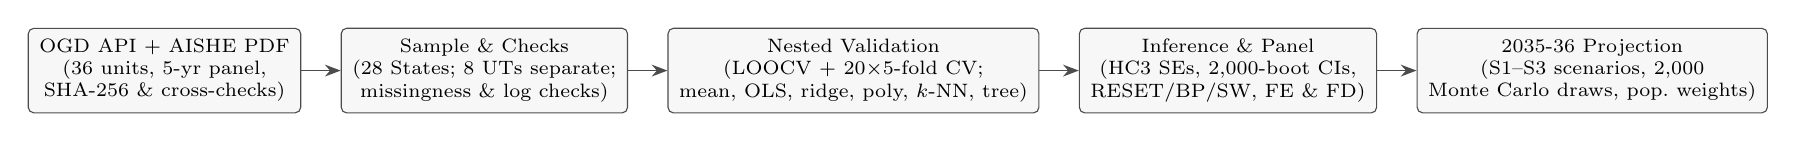
\begin{tikzpicture}[
  node distance=5mm and 5mm,
  box/.style={rectangle, rounded corners=2pt, draw=black!70, fill=black!3, align=center, font=\scriptsize, inner sep=4pt, minimum height=9mm},
  arr/.style={-{Stealth[length=2mm]}, semithick, draw=black!70}
]
\node[box] (data) {OGD API + AISHE PDF\\(36 units, 5-yr panel,\\SHA-256 \& cross-checks)};
\node[box, right=of data] (sample) {Sample \& Checks\\(28 States; 8 UTs separate;\\missingness \& log checks)};
\node[box, right=of sample] (cv) {Nested Validation\\(LOOCV + $20{\times}5$-fold CV;\\mean, OLS, ridge, poly, $k$-NN, tree)};
\node[box, right=of cv] (diag) {Inference \& Panel\\(HC3 SEs, 2,000-boot CIs,\\RESET/BP/SW, FE \& FD)};
\node[box, right=of diag] (proj) {2035-36 Projection\\(S1--S3 scenarios, 2,000\\Monte Carlo draws, pop.\ weights)};
\draw[arr] (data) -- (sample);
\draw[arr] (sample) -- (cv);
\draw[arr] (cv) -- (diag);
\draw[arr] (diag) -- (proj);
\end{tikzpicture}}
\caption{End-to-end workflow linking official data validation, nested cross-validation, panel sensitivity checks and change-based 2035-36 projections. Source: \texttt{src/run\_all.py}.}
\label{fig:workflow}
\end{figure}

\subsection{Notation and baseline}

Let \(y_s\) be the GER of State \(s\) in 2021-22 and let \(D_s\), \(P_s\) and \(G_s\) denote college density, PTR and GPI. The benchmark is the mean predictor, which assigns every State the training-sample mean:
\[
\hat{y}_s = \bar{y}_{\text{train}}.
\]
The baseline is not a straw man. With \(n = 28\), it is a demanding test: a model that cannot beat the mean out of sample has no predictive content, however impressive its in-sample \(R^2\).

\subsection{Linear model and OLS}

The primary specification is
\[
y_s = \beta_0 + \beta_D D_s + \beta_P P_s + \beta_G G_s + \varepsilon_s.
\]
OLS chooses the coefficient vector \(\beta = (\beta_0, \beta_D, \beta_P, \beta_G)'\) that minimises the residual sum of squares:
\[
\hat{\beta} = \arg\min_{\beta} \sum_s \left(y_s - x_s'\beta\right)^2 = (X'X)^{-1}X'y,
\]
where \(x_s = (1, D_s, P_s, G_s)'\). The model is estimated on the raw scale for interpretability. HC3 hetero\-skedasticity-robust standard errors are reported because the Breusch--Pagan test is a diagnostic, not a licence to assume homoskedasticity \cite{white1980,mackinnon1985}. Coefficient uncertainty is also summarised with 2,000 bootstrap resamples of the 28 States, using percentile intervals \cite{efron1993}. Standardised coefficients (SD of GER per SD of predictor) make the effect sizes comparable, and VIFs diagnose collinearity.

\subsection{Ridge regression}

Ridge adds an \(L_2\) penalty to the least-squares objective:
\[
\hat{\beta}_{\text{ridge}} = \arg\min_{\beta} \sum_s \left(y_s - x_s'\beta\right)^2 + \lambda \sum_{j \in \{D,P,G\}} \beta_j^2.
\]
The penalty shrinks coefficients toward zero and stabilises them when predictors are correlated \cite{hoerl1970}. The intercept is not penalised. Features are standardised before the penalty is applied, so \(\lambda\) is comparable across variables. \(\lambda\) is selected by \texttt{RidgeCV} over 61 log-spaced values from \(10^{-3}\) to \(10^{3}\), using efficient leave-one-out generalised cross-validation inside each training fold. The selected value on the full sample is \(\lambda = 7.943\).

\subsection{Polynomial ridge}

The polynomial specification expands the three features into all squares and pairwise products, then applies ridge:
\[
\hat{y} = \beta_0 + \sum_{j=1}^3 \beta_j x_j + \sum_{1 \le j \le k \le 3} \beta_{jk} x_j x_k.
\]
This is a flexible predictive benchmark that can capture diminishing returns or interactions. Degrees 1, 2 and 3 were compared by LOOCV; degree 2 performed best (RMSE 5.96, against 6.74 for degree 1 and 6.57 for degree 3). The degree-2 model is reported. It is not used for projection because its fitted curve turns downward beyond roughly 45--66 colleges per lakh, implying that further expansion eventually reduces GER. That is an extrapolation artefact, not a policy finding.

\subsection{Non-parametric benchmarks}

Two tuned non-parametric models test whether a flexible learner can do better with the same three features. \(k\)-nearest-neighbour regression averages the outcomes of the \(k\) closest training States under Euclidean distance; the search covers \(k \in \{3,5,7,9,11,15\}\) and uniform or distance weighting. A regression tree recursively partitions the feature space to minimise within-node squared error; the search covers maximum depth \(\in \{2,3,4\}\) and minimum leaf size \(\in \{3,5\}\). Both searches use LOOCV and root mean squared error, and both are repeated inside every outer fold of the model comparison. The nested design is important: tuning on the full sample and then evaluating on the same sample would overstate performance.

\subsection{Validation design}

Because \(n = 28\), leave-one-out cross-validation is the primary out-of-sample criterion \cite{stone1974}. Each State is held out once, the model is refitted on the other 27, and the held-out prediction is compared with the observed GER. The reported metrics are \(R^2\), RMSE and MAE. \(R^2\) is computed on the pooled out-of-sample predictions, so it can be negative when a model is worse than the mean.

A single partition can flatter or penalise a model by chance. Each specification is therefore also evaluated with 20 repeats of shuffled five-fold cross-validation. The mean and standard deviation of RMSE across repeats are reported. The two protocols answer different questions: LOOCV is the most efficient use of 28 observations, while repeated five-fold CV shows how sensitive the ranking is to the composition of the folds. Hyper-parameter tuning is nested inside both protocols, so no held-out State influences scaling, penalty selection or neighbour choice.

\subsection{Diagnostics and influence}

Residual diagnostics include the Shapiro--Wilk test for normality \cite{shapiro1965}, the Breusch--Pagan test for heteroskedasticity \cite{breusch1979}, the Ramsey RESET test for functional form \cite{ramsey1969}, and the condition number of the design matrix. Influence is measured with leverage, studentised residuals, DFFITS and Cook's distance \cite{cook1977}. The conventional Cook's distance threshold is \(4/n = 0.143\). Two States exceed it: Karnataka and Nagaland. The model is re-estimated without them to check that the college density result is not driven by one or two observations.

\subsection{Panel and sensitivity checks}

A short panel is used to ask whether the cross-sectional pattern survives within-State variation. Three specifications are estimated:

\begin{itemize}
  \item \textbf{Year fixed effects.} Pooled OLS with year dummies and State-clustered standard errors. Identification comes from within-State changes plus a common annual shift.
  \item \textbf{State and year fixed effects.} Adds State dummies, so identification comes only from within-State changes over time.
  \item \textbf{First differences.} Regresses the annual change in GER on annual changes in college density, PTR and GPI, removing any time-invariant State characteristic.
\end{itemize}

The year fixed-effects model also provides the common annual trend used in the projection: the coefficient on 2021-22 divided by four years, with its cluster-robust standard error. A UT-inclusive sensitivity model (35 units, with and without a UT dummy) documents the cost of pooling UTs with States.

\subsection{Projection to 2035-36}\label{sec:projection}

The cross-section predicts State GER in the same year (2021-22) from college density, PTR and GPI; it is not a time-series model. Turning it into a 2035 projection requires four assumptions: (i) the conditional associations are stable over 2022--2035; (ii) college density, PTR and GPI follow the scenario paths in Table~\ref{tab:scenarios}; (iii) the common annual participation trend of 0.866 points continues; and (iv) State-specific shocks are additive and can be represented by draws from the residual distribution. Under these assumptions the output is a conditional forecast, not a causal prediction of what any single policy will achieve.

The projection is change-based, not level-based:
\begin{equation}
\begin{aligned}
\GER_{s,2035} = \GER_{s,2021} &+ \beta_D (D_{s,2035} - D_{s,2021}) + \beta_P (P_{s,2035} - P_{s,2021}) \\
&+ \beta_G (G_{s,2035} - G_{s,2021}) + \tau h m,
\end{aligned}
\label{eq:projection}
\end{equation}
where \(h = 14\) years, \(m\) is a scenario-specific trend multiplier, and \(\tau = 0.866\) GER points per year (SE 0.174) is the common trend from the year fixed-effects panel. The coefficients \((\beta_D, \beta_P, \beta_G)\) are the OLS estimates from the 28-State cross-section. The intercept \(\beta_0\) is deliberately excluded: a cross-sectional intercept would embed the 2021-22 level permanently and would forecast that a State with average predictors stays at the sample average forever.

Three scenarios are defined in Table~\ref{tab:scenarios}. S1 damps both college density growth and the common trend; S2 carries recent trends forward and is the reference case; S3 adds teacher and parity convergence to full college density growth.

\begin{table}[htbp]
\centering
\scriptsize
\setlength{\tabcolsep}{3pt}
\caption{Scenario definitions used in the 2035-36 projection. All scenarios use the OLS coefficients \((\beta_D, \beta_P, \beta_G)\) from the 28-State cross-section, the common annual trend \(\tau\) from the year fixed-effects panel, and a college density cap of 100 colleges per lakh. The recent annual density change is the 2017-18 to 2021-22 change divided by four. Source: \texttt{src/projection.py}.}
\label{tab:scenarios}
\begin{tabular}{@{}p{2.9cm}p{2.7cm}p{2.8cm}p{2.9cm}@{}}
\toprule
Assumption & S1 Damped & S2 Recent trend (ref.) & S3 NEP reform \\
\midrule
Annual density change & \(0.5 \times\) recent & \(1.0 \times\) recent & \(1.0 \times\) recent \\
Common trend & \(0.5 \times \tau\) & \(\tau\) & \(\tau\) \\
PTR (\(P_{s,2035}\)) & unchanged (\(P_{s,2021}\)) & unchanged (\(P_{s,2021}\)) & \(\min(P_{s,2021},20)\) \\
GPI (\(G_{s,2035}\)) & unchanged (\(G_{s,2021}\)) & unchanged (\(G_{s,2021}\)) & \(\max(G_{s,2021}, 1.05)\) \\
Density bounds & 1 to 100 & 1 to 100 & 1 to 100 \\
\bottomrule
\end{tabular}
\end{table}

The recent annual college density change is the 2017-18 to 2021-22 change divided by four. College density is capped at 100 colleges per lakh and floored at 1.

Uncertainty is propagated with 2,000 bootstrap draws. In each draw, the 28 States are resampled with replacement, the OLS coefficients are re-estimated, the common trend is drawn from \(N(0.866, 0.174)\), and a State-level residual is drawn from \(N(0, 6.315)\). The same draws are used across scenarios (common random numbers), so differences between scenarios are not confounded by Monte Carlo noise. \(P(\GER \ge 50\%)\) is the share of draws at or above the target, and the 5th--95th percentile interval is reported. States are classified as Achieved (GER already \(\ge 50\%\)), On track (\(P(\GER \ge 50\%) \ge 0.5\)), At risk (\(0.15 \le P(\GER \ge 50\%) < 0.5\)) or Off track (\(P(\GER \ge 50\%) < 0.15\)). The 0.5 cut-off is a communication device, not a statistical test; the probability itself is the more informative quantity.

\subsection{Required density}

For each State, the model-implied college density required by 2035-36 under S2 is obtained by solving equation~\eqref{eq:projection} for \(D_{s,2035}\) with \(\GER_{s,2035} = 50\) and PTR and GPI held at their 2021-22 values:
\begin{equation}
D_s^{\text{req}} = D_{s,2021} + \frac{50 - \left(\GER_{s,2021} + \tau h\right)}{\beta_D}.
\label{eq:required}
\end{equation}
The density gap is \(\max(0, D_s^{\text{req}} - D_{s,2035})\). An indicative additional-college figure multiplies the gap by the implied 18--23 population (\(\text{colleges}_{s,2021} / D_{s,2021}\)). This is a model-implied illustration, not a costing. It assumes that the linear density coefficient \(\beta_D\) applies far outside the observed range and ignores teacher supply, land, funding and demand.

\subsection{Software and reproducibility}

The analysis uses Python 3.14.4 with pandas 3.1.0, NumPy 2.5.4, scikit-learn 1.9.1, statsmodels 0.15.0, SciPy 1.18.1, matplotlib 3.11.2, seaborn 0.13.2, pypdf 6.21.4, pdfplumber 0.11.10 and openpyxl 3.1.5. Exact versions are pinned in \path{requirements.txt}. The random seed is 42 for every stochastic step. \path{src/run_all.py} runs the pipeline end to end (including \path{src/checks.py}); individual scripts can be run separately. All tables are written to \path{outputs/tables/} and all figures to \path{outputs/figures/} at 300 dpi. \path{src/verify_outputs.py} re-reads the artefacts and checks the headline numbers quoted in this article, so a reader can distinguish a reproduction failure from a typo.

\section{Experimental Setup}\label{sec:setup}

\textbf{Sample.} 28 States, 2021-22 cross-section, with no missing values on the three core predictors. The panel has 140 State-year observations for the year fixed-effects model (28 States $\times$ 5 years) and 112 first differences.

\textbf{Split.} The cross-section is evaluated by LOOCV. There is no random train/test split because, with 28 units, a single split would be too sensitive to which States happen to land in the test set. The repeated five-fold protocol provides the stability check.

\textbf{Tuning.} Hyper-parameters are selected inside each training fold. Table~\ref{tab:tuning} lists the grids, the selection rule and the values selected on the full sample. The nested LOOCV column is the honest score; the internal score is shown only to make the optimism of non-nested tuning visible.

\textbf{Environment.} Python 3.14.4, scikit-learn 1.9.1, statsmodels 0.15.0, pandas 3.1.0, NumPy 2.5.4, SciPy 1.18.1 and matplotlib 3.11.2, all pinned in \path{requirements.txt}. The pipeline runs on Windows and Linux; \path{run.sh} is provided for Linux and \path{README.md} documents both. Figures use the Matplotlib ``DejaVu Sans'' font and a colour-blind-safe palette.

\textbf{Reporting conventions.} Tables are numbered in the order in which they are cited. Each table caption names the CSV file in \path{outputs/tables/} that contains the same numbers, so the narrative and the artefacts can be cross-checked. Figures are embedded at print resolution. All percentages are GER points unless stated otherwise.

\section{Results}\label{sec:results}

\subsection{Descriptive patterns}

Table~\ref{tab:descriptives} summarises the estimation sample. Mean GER is 30.4\%, with a standard deviation of 8.8 points. The distribution is wide and slightly left-skewed: the median (30.6\%) is close to the mean, but the minimum (16.9\%) is further below the median than the maximum (47.0\%) is above it. Fourteen States are below 30\%, and none has reached 50\%. College density averages 31.0 colleges per lakh, with a range from 7 in Bihar to 66 in Karnataka. PTR averages 24.6 and ranges from 14 in Tamil Nadu to 64 in Bihar. GPI averages 1.06, with ten States below parity and seven at or above 1.2.

\begin{table}[htbp]
\centering
\small
\caption{Descriptive statistics, 28 States, 2021-22. Average enrolment per college is shown for reference and is used only in a robustness model. Source: \texttt{table01\_summary\_statistics.csv}.}
\label{tab:descriptives}
\begin{tabular}{@{}lrrrrr@{}}
\toprule
Variable & Mean & SD & Min & Median & Max \\
\midrule
GER (\%) & 30.4 & 8.8 & 16.9 & 30.6 & 47.0 \\
College density (per lakh 18--23) & 31.0 & 13.7 & 7.0 & 29.0 & 66.0 \\
Pupil--teacher ratio & 24.6 & 11.5 & 14.0 & 22.5 & 64.0 \\
Gender Parity Index & 1.06 & 0.15 & 0.88 & 1.02 & 1.44 \\
Average enrolment per college & 800 & 394 & 413 & 668 & 2,088 \\
\bottomrule
\end{tabular}
\end{table}

Table~\ref{tab:correlations} reports Pearson and Spearman correlations. Density has the strongest positive association with GER (\(r = 0.712\); \(\rho = 0.751\)), followed by PTR with a negative association (\(r = -0.612\); \(\rho = -0.645\)). GPI is weakly associated (\(r = 0.189\); \(\rho = 0.173\)), and average enrolment per college is negatively associated (\(r = -0.460\)). Density and PTR are themselves correlated at \(-0.66\), which is why the multivariate density coefficient is smaller than the bivariate slope.

\begin{table}[htbp]
\centering
\small
\caption{Correlations with GER, 28 States, 2021-22. Pearson and Spearman coefficients; the Spearman coefficient for average enrolment is not reported because the variable is used only as a robustness check. Source: \texttt{table02\_correlations.csv} and \texttt{table02b\_spearman.csv}.}
\label{tab:correlations}
\begin{tabular}{@{}lrr@{}}
\toprule
Variable & Pearson \(r\) & Spearman \(\rho\) \\
\midrule
College density & 0.712 & 0.751 \\
Pupil--teacher ratio & $-0.612$ & $-0.645$ \\
Gender Parity Index & 0.189 & 0.173 \\
Average enrolment per college & $-0.460$ & --- \\
\bottomrule
\end{tabular}
\end{table}

\begin{figure}[htbp]
\centering
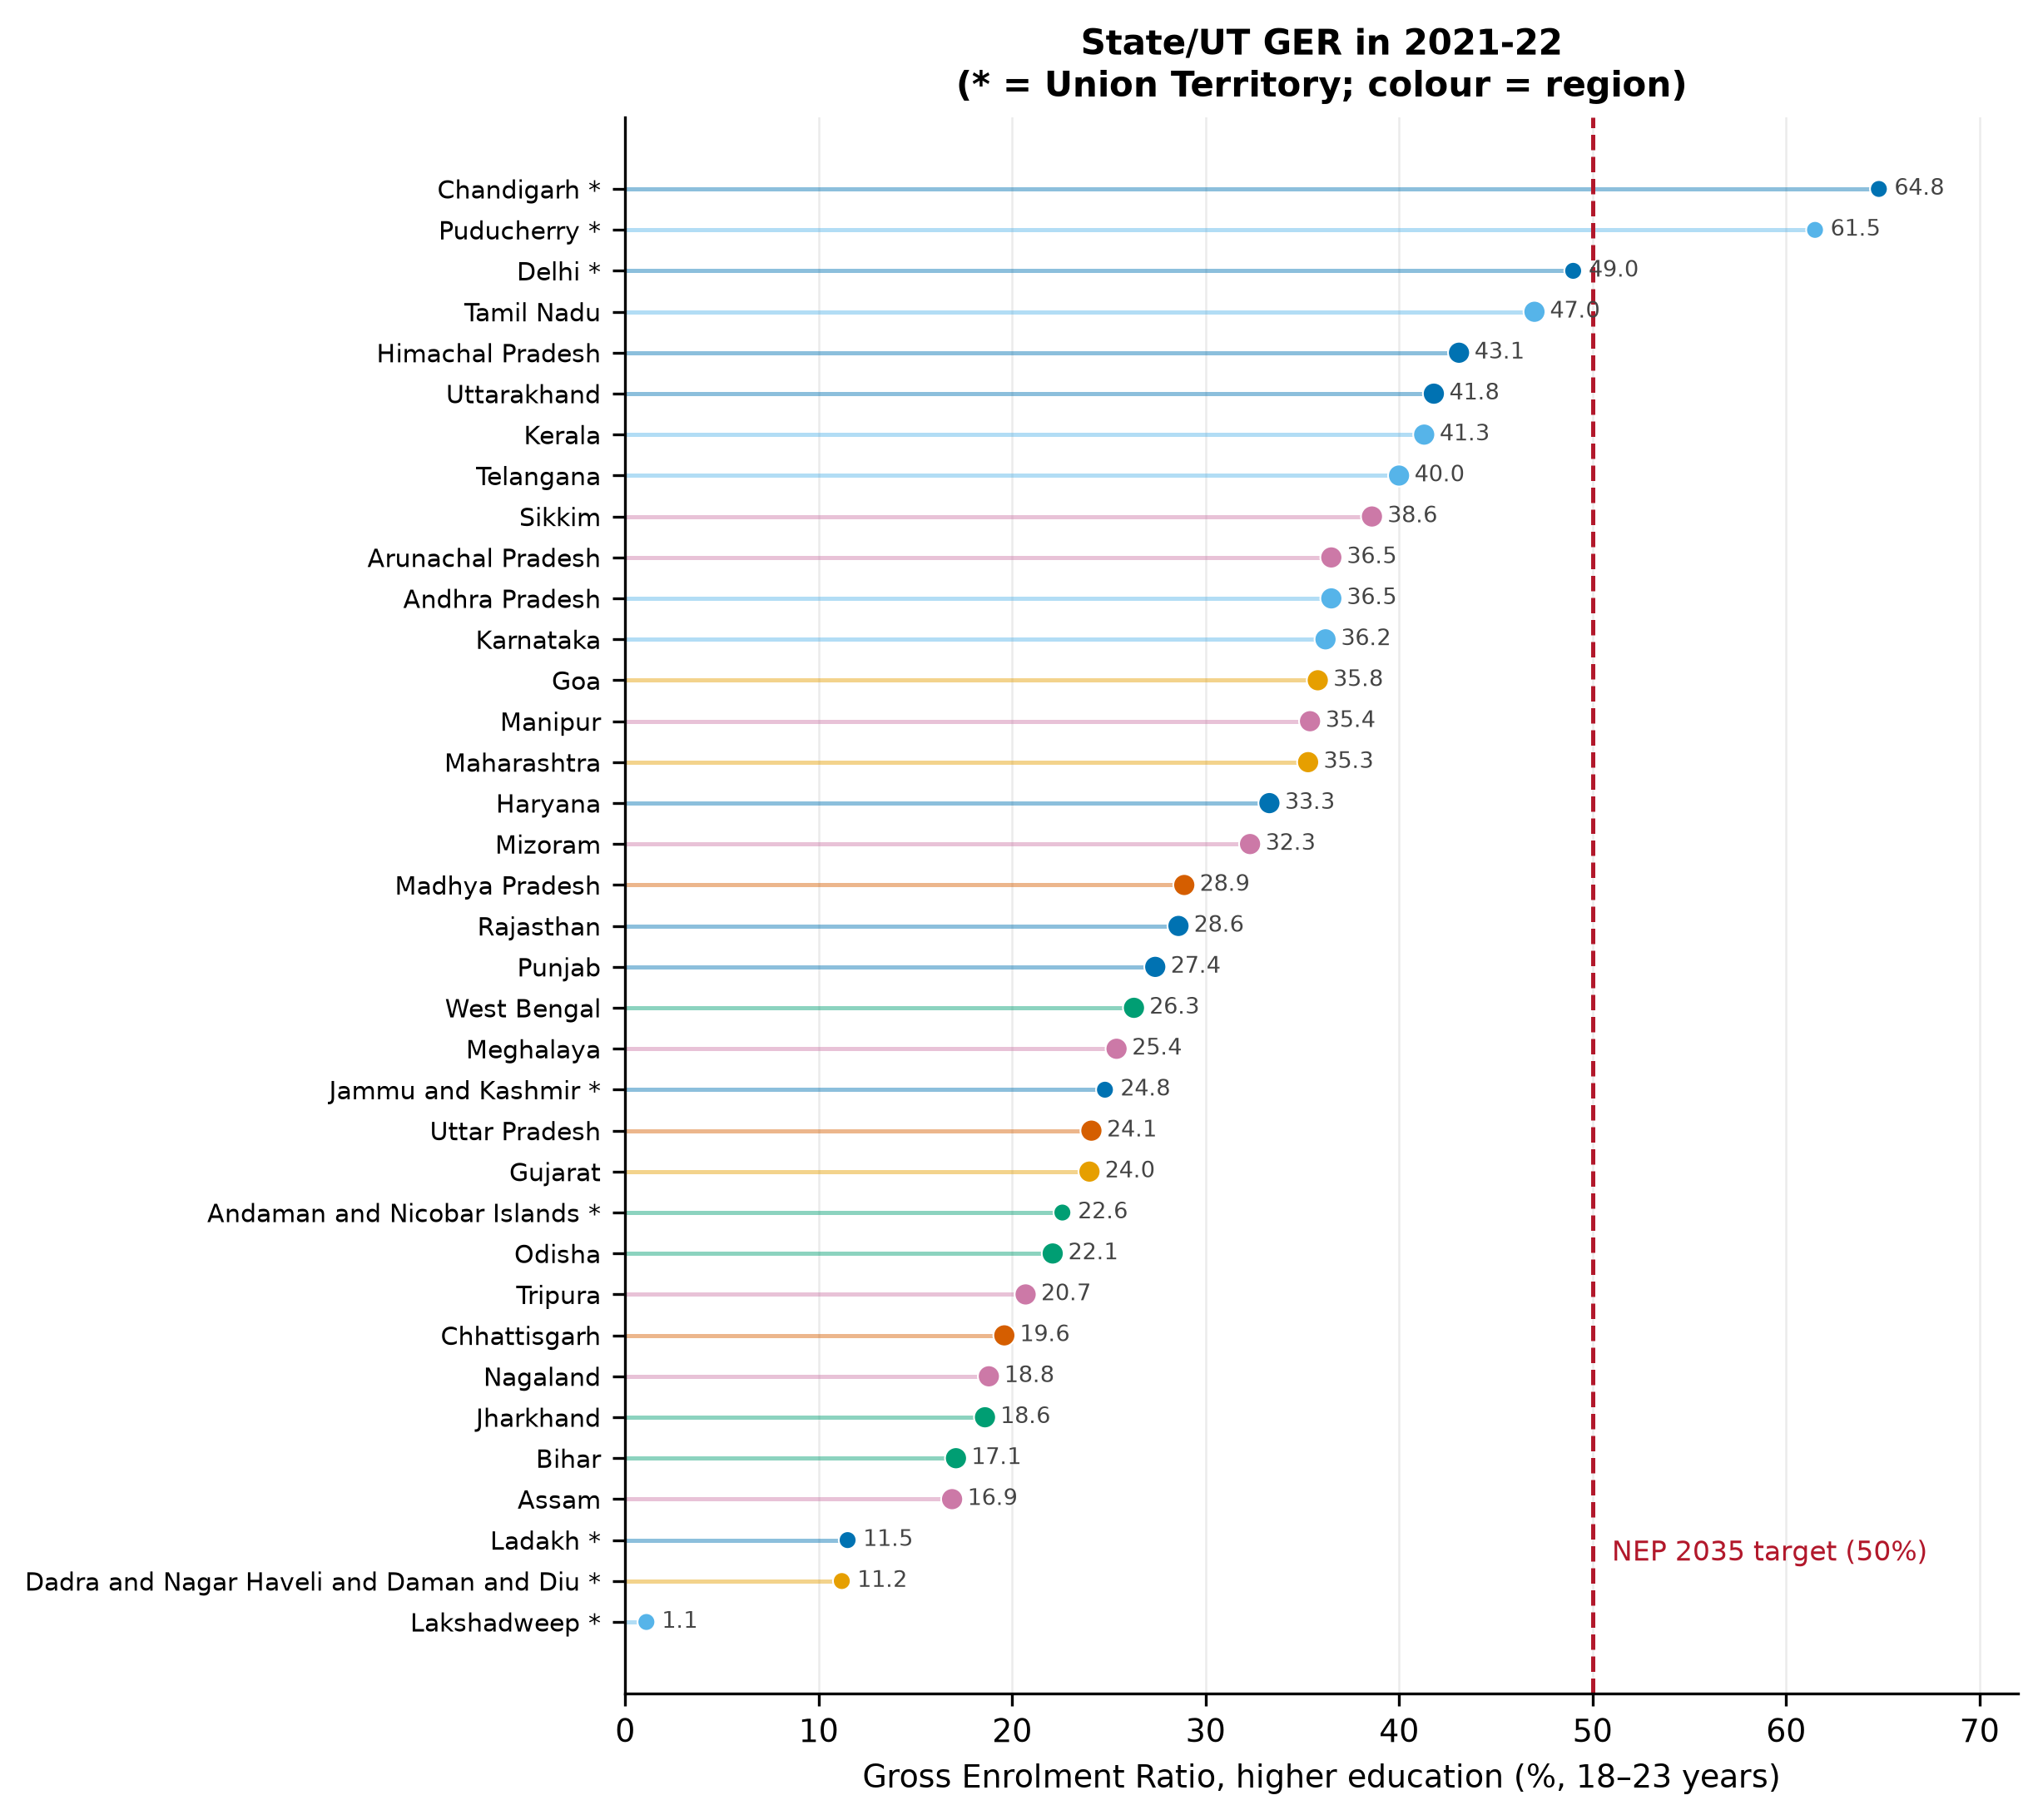
\includegraphics[width=0.86\linewidth]{fig01_ger_ranked.png}
\caption{State and Union Territory GER in 2021-22, ranked. The southern and hilly States cluster at the top; the Gangetic plain and the Northeast contain most of the low-GER units. Union Territories are shown for context but are excluded from estimation. Source: \texttt{fig01\_ger\_ranked.png}.}
\label{fig:ranked}
\end{figure}

Figure~\ref{fig:ranked} shows the full ranking of 36 units. Tamil Nadu (47.0), Himachal Pradesh (43.1), Uttarakhand (41.8), Kerala (41.3) and Telangana (40.0) lead the States. Assam (16.9), Bihar (17.1), Jharkhand (18.6), Nagaland (18.8), Chhattisgarh (19.6), Tripura (20.7), Odisha (22.1) and Uttar Pradesh (24.1) trail. The UTs are a separate distribution: Chandigarh (64.8), Puducherry (61.5) and Delhi (49.0) are high, while Dadra and Nagar Haveli and Daman and Diu (11.2) is the lowest unit in the file.

\begin{figure}[htbp]
\centering
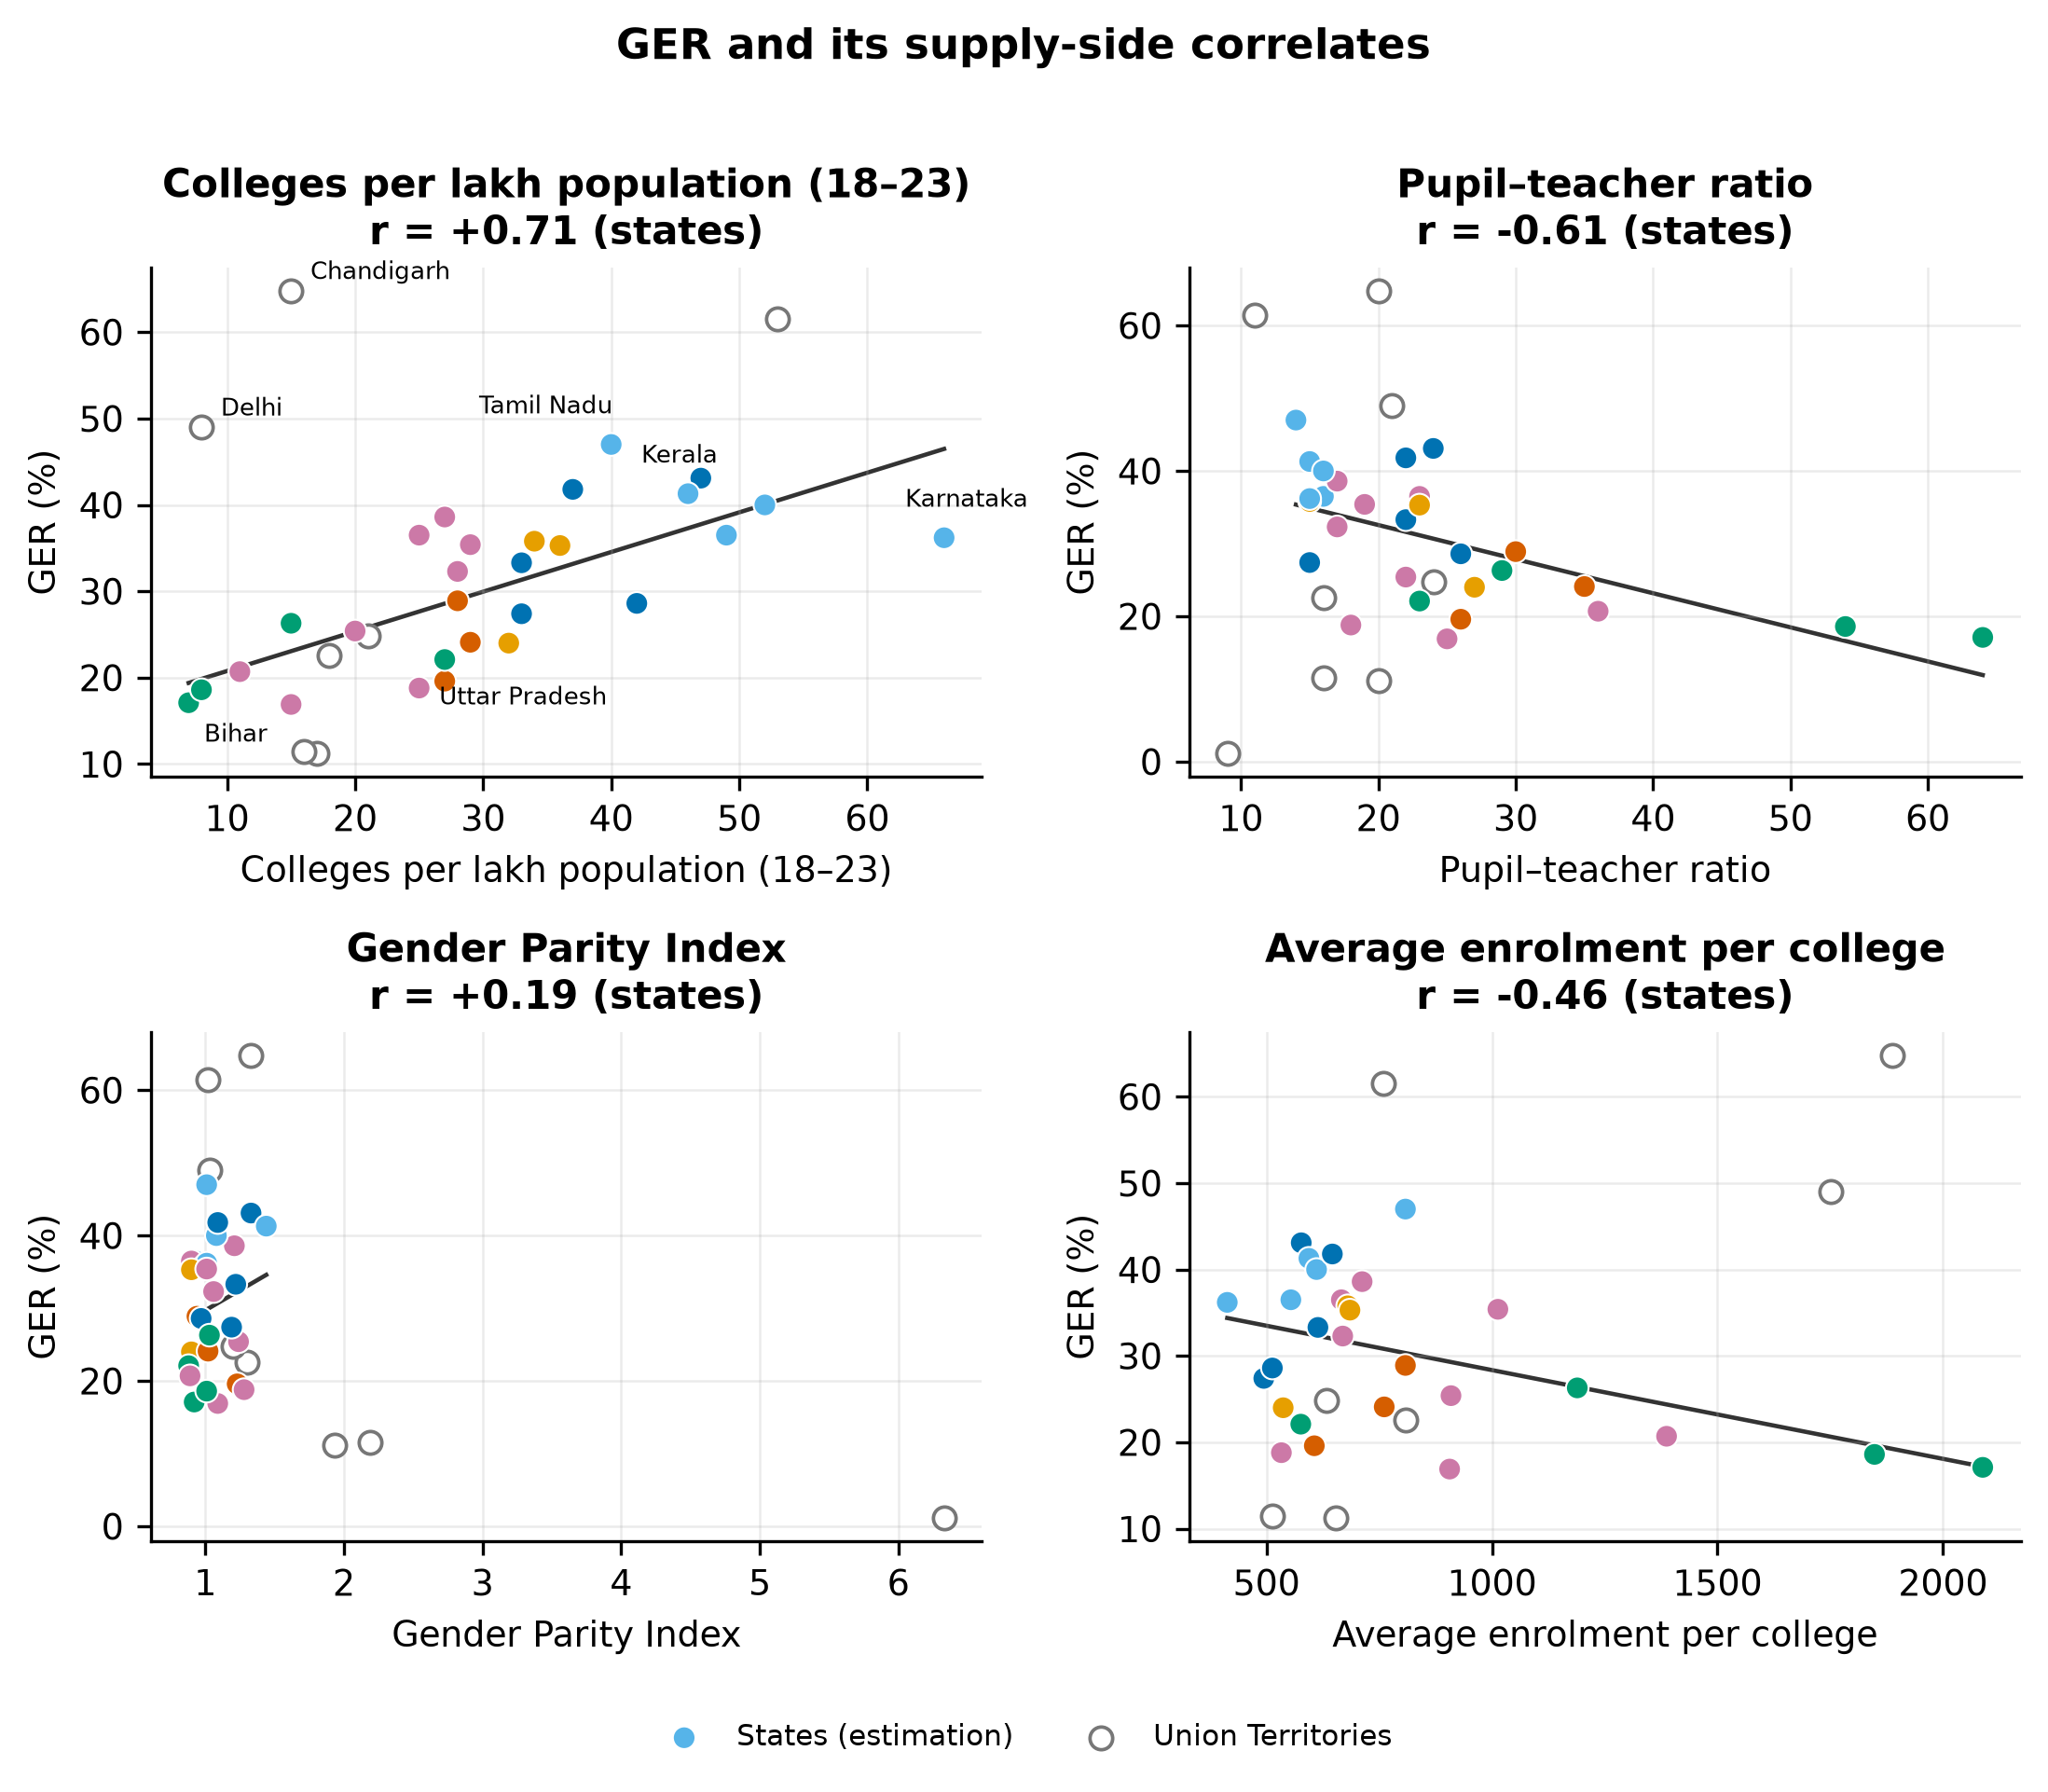
\includegraphics[width=\linewidth]{fig02_correlates.png}
\caption{GER against the four candidate correlates, 28 States, 2021-22. Density is positively associated, PTR negatively, GPI weakly, and average enrolment per college negatively. Source: \texttt{fig02\_correlates.png}.}
\label{fig:correlates}
\end{figure}

Figure~\ref{fig:correlates} makes the bivariate patterns visible and also shows why a multivariate model is needed. The density relationship is tight but has notable exceptions: Karnataka has the highest density (66) but a GER of only 36.2, while Tamil Nadu reaches 47.0 with a density of 40. The PTR relationship is negative but is driven partly by the low-density, high-PTR States. The GPI panel is almost flat. Average enrolment per college is negatively related to GER, which is a warning that college size is not a quality proxy: Bihar combines the largest average college (2,088 students) with the lowest density and a GER of 17.1.

\begin{figure}[htbp]
\centering
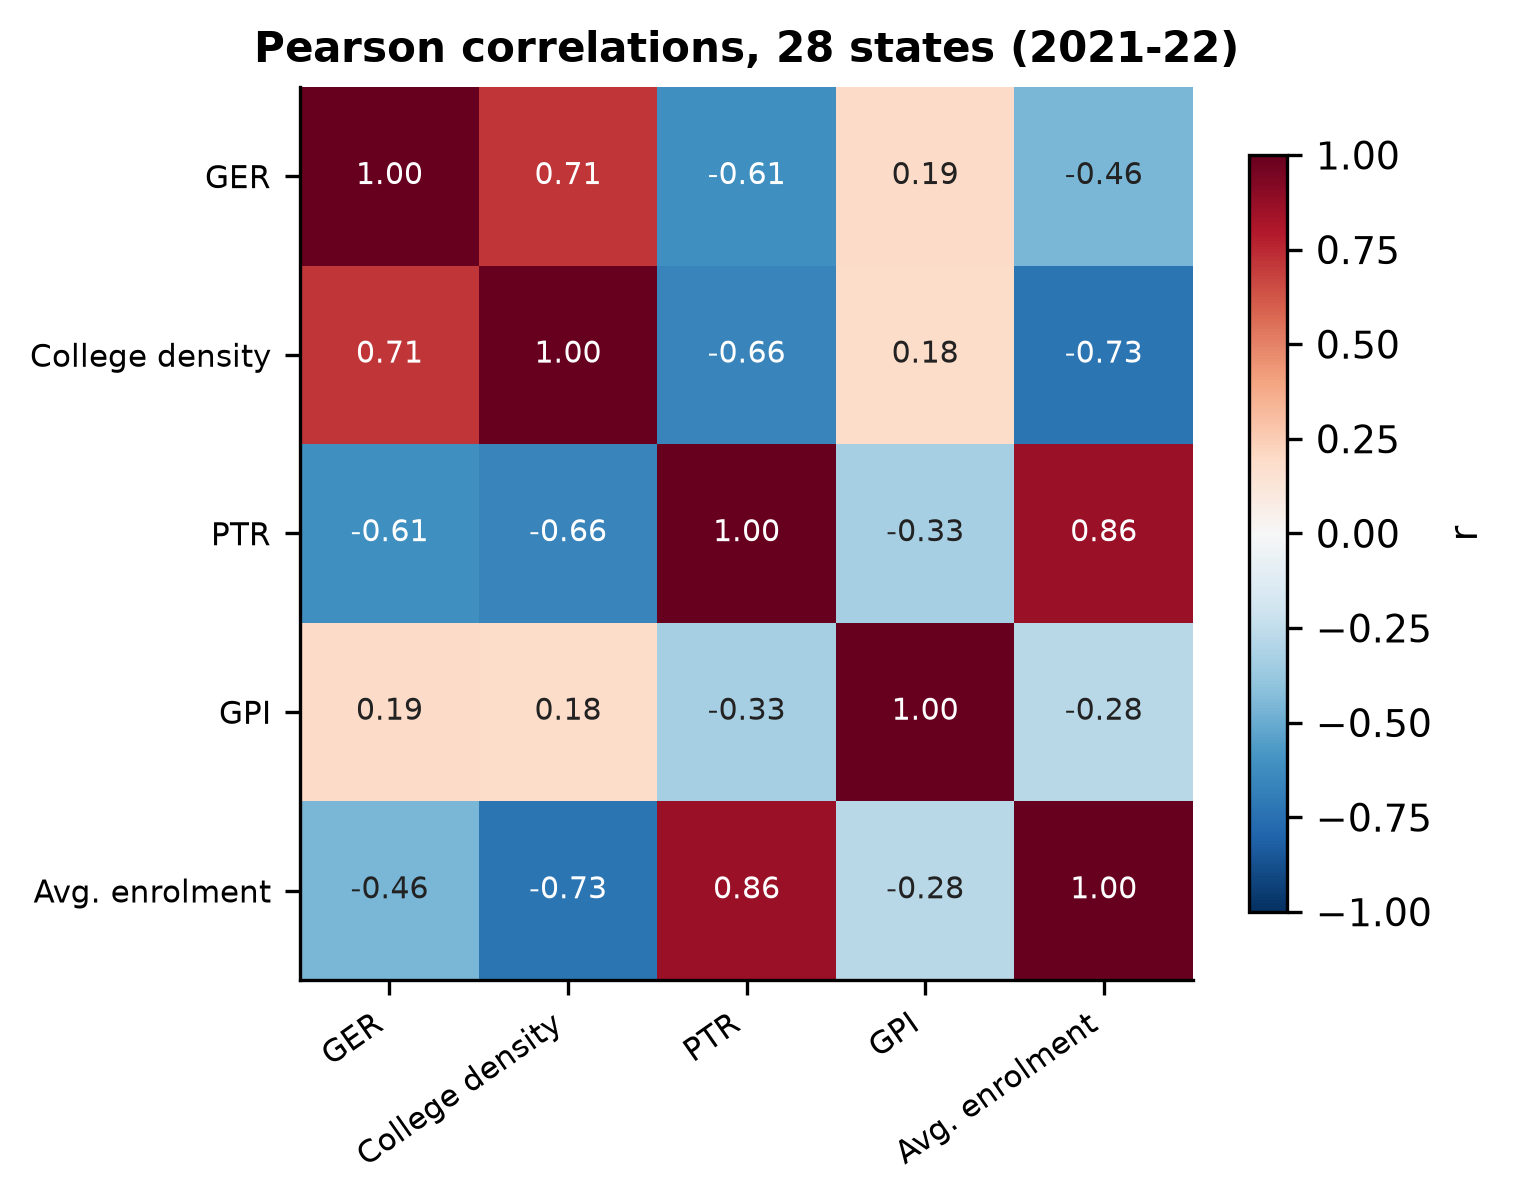
\includegraphics[width=0.82\linewidth]{fig03_correlation_heatmap.png}
\caption{Pearson correlation matrix for GER and its correlates, 28 States, 2021-22. Density and PTR are strongly negatively correlated; GPI is weakly correlated with both. Source: \texttt{fig03\_correlation\_heatmap.png}.}
\label{fig:heatmap}
\end{figure}

\begin{figure}[htbp]
\centering
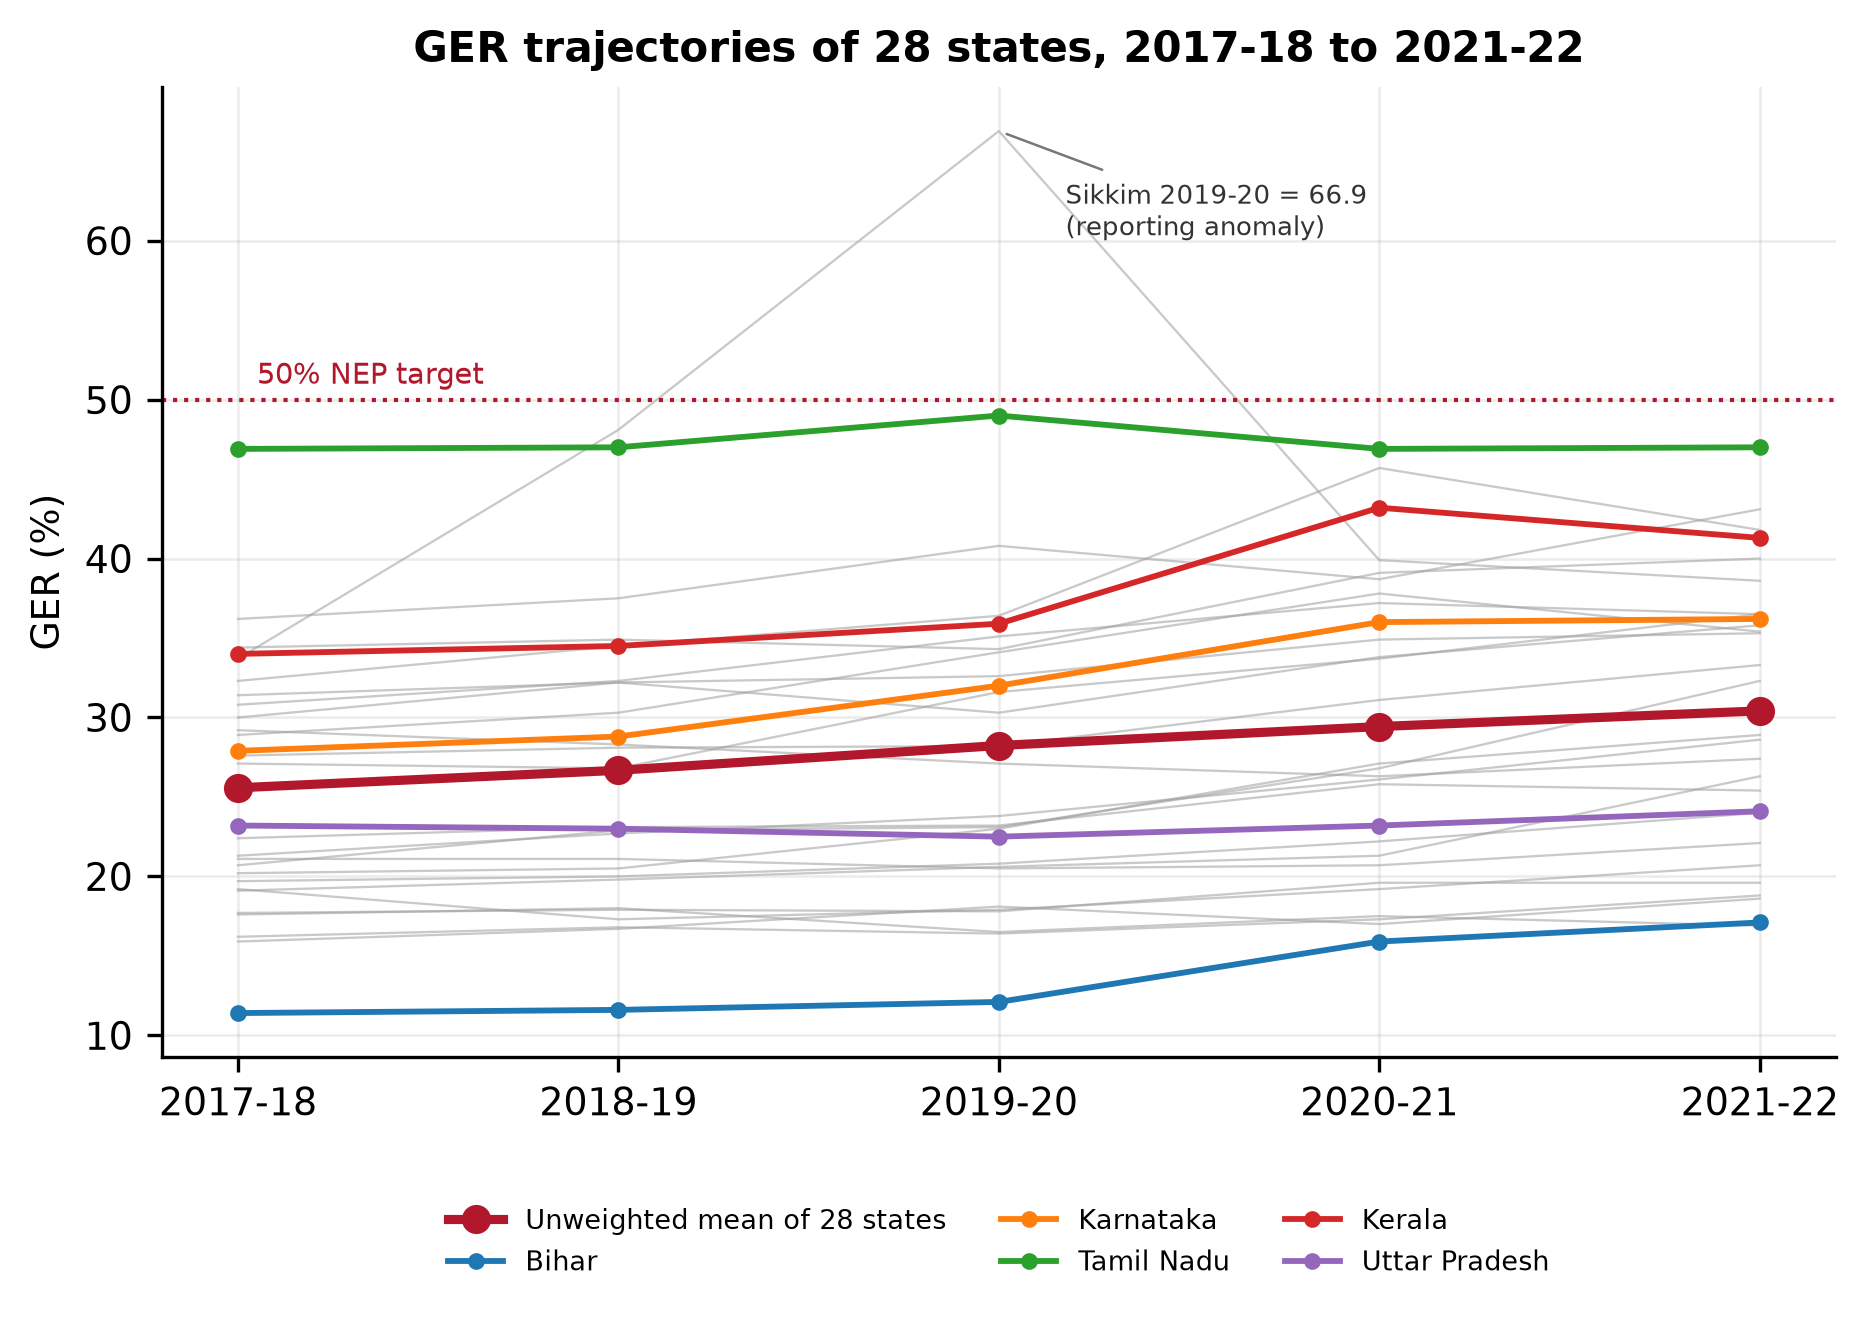
\includegraphics[width=\linewidth]{fig04_trajectories.png}
\caption{GER trajectories, 2017-18 to 2021-22. Most States improved, but the gap between the top and bottom groups persisted. The 2019-20 Sikkim observation is annotated as a reporting anomaly. Source: \texttt{fig04\_trajectories.png}.}
\label{fig:trajectories}
\end{figure}

Figure~\ref{fig:heatmap} confirms the density--PTR collinearity and the weak GPI--GER association. Figure~\ref{fig:trajectories} shows that the level differences are persistent: the States at the top in 2017-18 are mostly at the top in 2021-22, and the bottom group improves from a lower base. This persistence is why a cross-sectional model has explanatory power and why a change-based projection is more defensible than a level forecast.

\subsection{Model comparison}

Table~\ref{tab:tuning} reports the hyper-parameter grids and the selected values. Table~\ref{tab:models} reports the model comparison. The polynomial ridge model has the lowest LOOCV RMSE (5.96) and the highest LOOCV \(R^2\) (0.525). OLS with college size is second (6.27; 0.474), followed by ridge with college size (6.42; 0.449), ridge with three indicators (6.74; 0.392) and OLS with three indicators (6.86; 0.370). The tuned tree (7.39; 0.269) and tuned \(k\)-NN (7.59; 0.229) are worse than OLS, despite much higher in-sample \(R^2\) (0.702 and 0.660). The baseline is worst (8.97; $-0.075$).

\begin{table}[htbp]
\centering
\caption{Hyper-parameter grids, selection rule and selected values. The ridge penalty \(\lambda\) corresponds to \texttt{alpha} in \texttt{RidgeCV}. The internal RMSE is the score seen by the search; the nested LOOCV RMSE is the honest out-of-sample score, with tuning repeated inside every outer fold. Source: \texttt{table10\_hyperparameter\_search.csv}.}
\label{tab:tuning}
\resizebox{\textwidth}{!}{%
\begin{tabular}{@{}llllrr@{}}
\toprule
Model & Grid searched & Selection rule & Selected & Internal RMSE & Nested RMSE \\
\midrule
Ridge (3 indicators) & \(\lambda\) in 61 log-spaced values, \(10^{-3}\) to \(10^{3}\) & RidgeCV GCV & \(\lambda = 7.943\) & 6.74 & 6.74 \\
Polynomial + ridge & degree \(\in \{1,2,3\}\); \(\lambda\) in 61 values & LOOCV (deg.); RidgeCV (\(\lambda\)) & degree 2; \(\lambda = 1.000\) & 5.96 & 5.96 \\
\(k\)-NN (tuned) & \(k \in \{3,5,7,9,11,15\}\); weights \(\in\) \{uniform, distance\} & GridSearchCV, LOOCV & \(k = 3\); uniform & 5.66 & 7.59 \\
Regression tree (tuned) & depth \(\in \{2,3,4\}\); min leaf \(\in \{3,5\}\) & GridSearchCV, LOOCV & depth 2; leaf 3 & 5.69 & 7.39 \\
\bottomrule
\end{tabular}}
\end{table}

Table~\ref{tab:tuning} is deliberately uncomfortable. The internal scores of the \(k\)-NN and tree searches (5.66 and 5.69) are much better than their nested LOOCV scores (7.59 and 7.39). The gap is the optimism of tuning and evaluating on the same 28 States. With \(n = 28\), a grid search can always find a hyper-parameter that fits the sample; the nested protocol reveals that the gain does not generalise. This is one reason the linear model is retained for inference and projection even though it is not the best predictor.

\begin{table}[htbp]
\centering
\caption{Model comparison, 28 States, 2021-22. LOOCV is the primary criterion; repeated five-fold CV is a stability check. The baseline assigns every State the training mean. Source: \texttt{table03\_model\_comparison.csv}.}
\label{tab:models}
\resizebox{\textwidth}{!}{%
\begin{tabular}{@{}lrrrrrr@{}}
\toprule
Model & LOOCV \(R^2\) & LOOCV RMSE & LOOCV MAE & 5-fold RMSE (mean $\pm$ SD) & In-sample \(R^2\) & Adj.\ \(R^2\) \\
\midrule
Polynomial deg 2 + ridge & \textbf{0.525} & \textbf{5.96} & \textbf{4.97} & 6.63 $\pm$ 0.73 & 0.730 & 0.696 \\
OLS (+ college size) & 0.474 & 6.27 & 4.82 & 6.58 $\pm$ 0.55 & 0.659 & 0.599 \\
Ridge (+ college size) & 0.449 & 6.42 & 4.95 & 6.81 $\pm$ 0.58 & 0.646 & 0.585 \\
Ridge (3 indicators) & 0.392 & 6.74 & 5.54 & 6.85 $\pm$ 0.25 & 0.528 & 0.469 \\
OLS (3 indicators) & 0.370 & 6.86 & 5.73 & 7.09 $\pm$ 0.37 & 0.543 & 0.486 \\
Regression tree (tuned) & 0.269 & 7.39 & 6.05 & 7.76 $\pm$ 0.69 & 0.702 & 0.665 \\
\(k\)-NN (tuned) & 0.229 & 7.59 & 6.52 & 7.32 $\pm$ 0.42 & 0.660 & 0.618 \\
Baseline (mean) & $-0.075$ & 8.97 & 7.95 & 9.00 $\pm$ 0.24 & 0.000 & $-0.125$ \\
\bottomrule
\end{tabular}}
\end{table}

Three points stand out. First, every learned model beats the mean baseline, but the margin is modest for the three-indicator OLS: LOOCV \(R^2\) is 0.370, not the 0.543 seen in-sample. The gap is expected with \(n = 28\) and three predictors, and it is a warning against reading the fitted values as forecasts. Second, ridge slightly improves out-of-sample error relative to OLS (6.74 vs 6.86) and shrinks the density coefficient from 0.353 to 0.271. The ranking is not an artefact of one partition: the repeated five-fold RMSE is also lower for ridge (6.85 vs 7.09). Third, the polynomial is the best predictor but the worst model to extrapolate. Figure~\ref{fig:poly} shows why.

The augmented model with average enrolment per college improves LOOCV \(R^2\) to 0.474, but average enrolment is mechanically related to GER: enrolment is the numerator of GER, and a State with a high GER can have a high average college size even if access is low. It is a robustness check, not the preferred specification.

\begin{figure}[htbp]
\centering
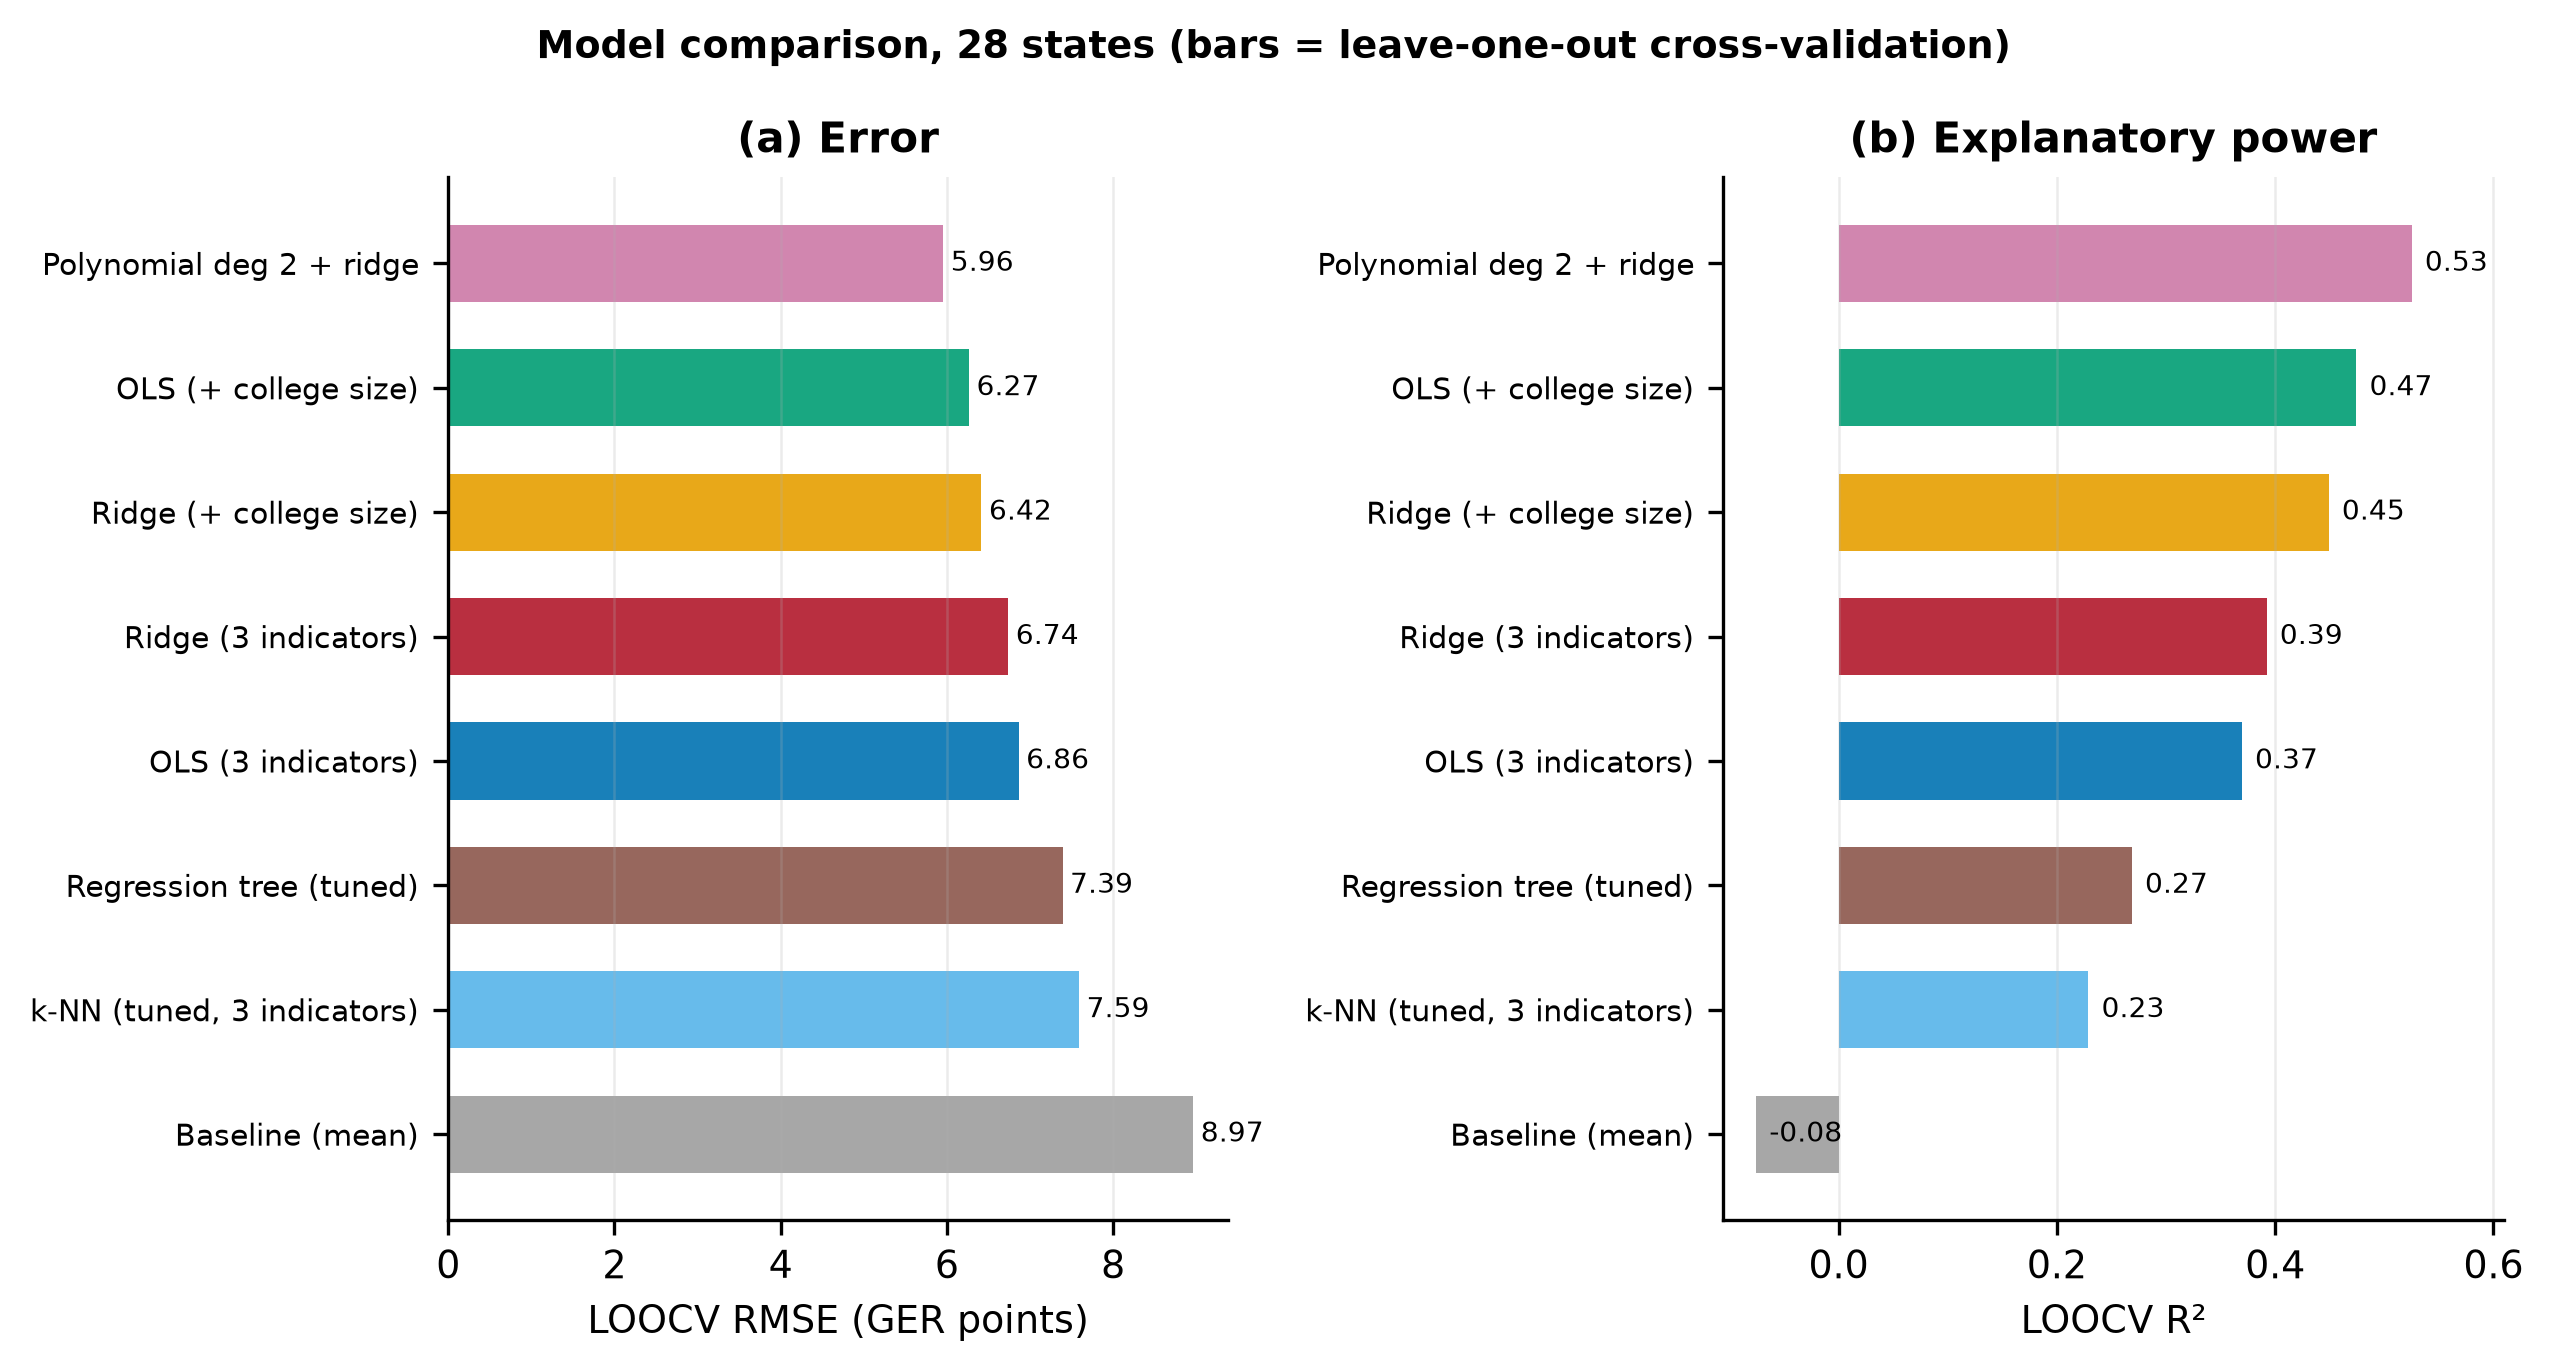
\includegraphics[width=\linewidth]{fig05_model_comparison.png}
\caption{LOOCV RMSE and \(R^2\) by model, 28 States. Lower RMSE and higher \(R^2\) are better. The polynomial ridge model is the best predictor; the tuned non-parametric models are worse than OLS out of sample. Source: \texttt{fig05\_model\_comparison.png}.}
\label{fig:modelcomp}
\end{figure}

\begin{figure}[htbp]
\centering
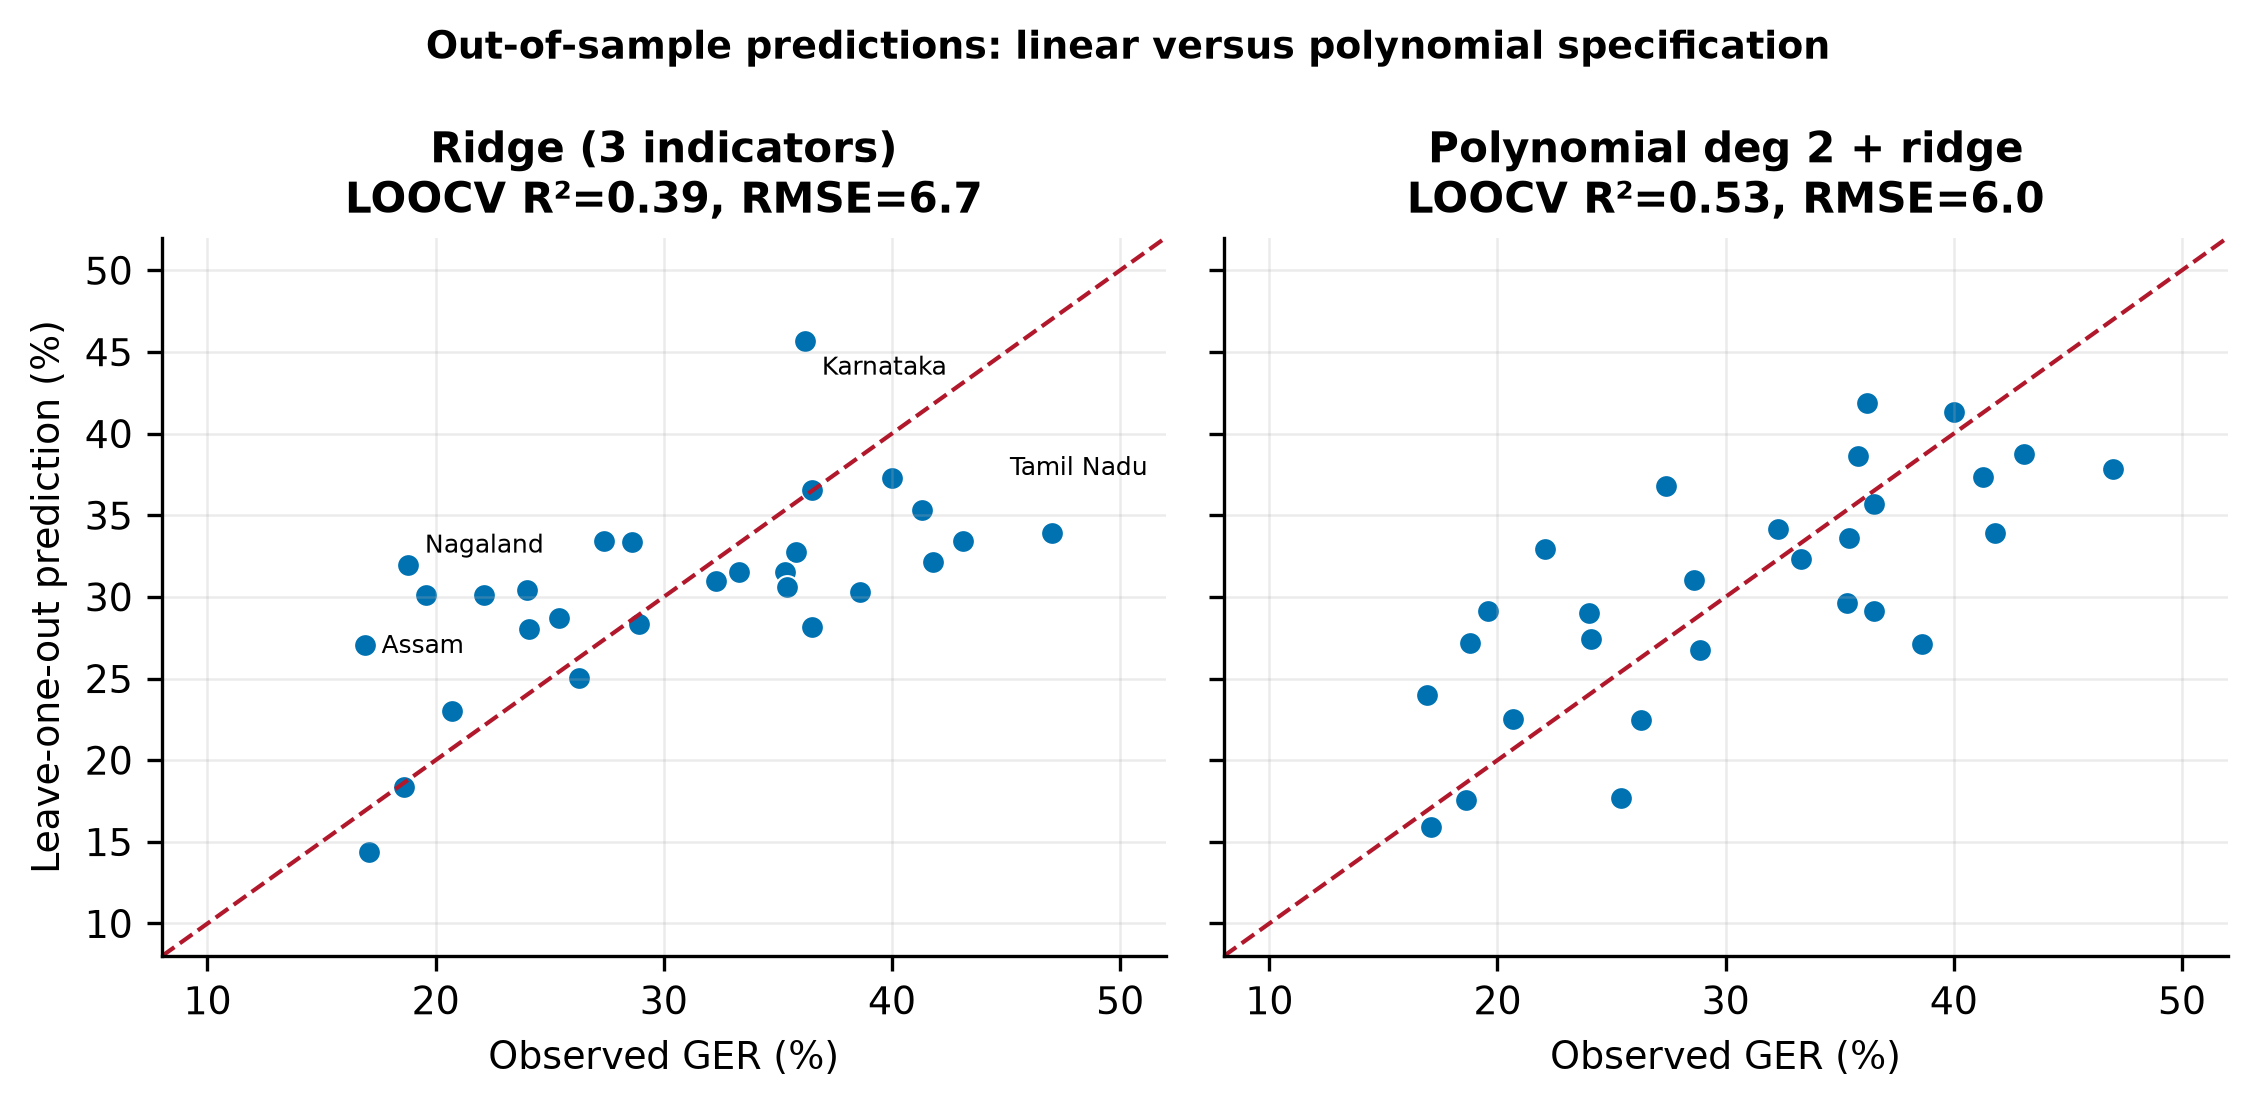
\includegraphics[width=\linewidth]{fig06_actual_vs_predicted.png}
\caption{Leave-one-out predictions against observed GER for ridge and polynomial ridge. The 45-degree line is perfect prediction. The polynomial tracks the middle of the distribution better but is less stable at the extremes. Source: \texttt{fig06\_actual\_vs\_predicted.png}.}
\label{fig:actualpred}
\end{figure}

Figure~\ref{fig:modelcomp} plots the two out-of-sample criteria, and Figure~\ref{fig:actualpred} shows that both models under-predict Tamil Nadu (47.0) and over-predict Karnataka (36.2), the two most influential States. The errors are not random: they reflect omitted variables such as private provision, urbanisation and demand, which are not in the three-indicator model.

\subsection{Coefficients and inference}

Table~\ref{tab:coefficients} reports the OLS coefficients with HC3 standard errors and bootstrap intervals. College density is the only coefficient that is statistically distinguishable from zero at conventional levels: \(+0.353\) GER points per additional college per lakh (HC3 SE 0.161; \(p = 0.029\); 95\% bootstrap interval 0.112 to 0.656). The standardised coefficient is 0.547, the largest in the model. Conditional on PTR and GPI, a one-standard-deviation increase in density is associated with about half a standard deviation of GER.

\begin{table}[htbp]
\centering
\caption{OLS coefficients, 28 States, 2021-22. HC3 standard errors; 95\% percentile bootstrap intervals from 2,000 resamples; standardised coefficients are SD of GER per SD of the predictor. Source: \texttt{table04\_coefficients.csv}.}
\label{tab:coefficients}
\resizebox{\textwidth}{!}{%
\begin{tabular}{@{}lrrrrrr@{}}
\toprule
Term & Coefficient & HC3 SE & \(p\)-value & Bootstrap 95\% CI & Standardised coefficient & VIF \\
\midrule
College density (\(\beta_D\)) & \textbf{0.353} & 0.161 & \textbf{0.029} & 0.112 to 0.656 & \textbf{0.547} & 1.78 \\
Pupil--teacher ratio (\(\beta_P\)) & $-0.189$ & 0.152 & 0.211 & $-0.637$ to 0.027 & $-0.247$ & 1.93 \\
Gender Parity Index (\(\beta_G\)) & 0.508 & 9.867 & 0.959 & $-22.46$ to 15.37 & 0.009 & 1.12 \\
\bottomrule
\end{tabular}}
\end{table}

The PTR coefficient is negative but imprecise: \(-0.189\) (\(p = 0.211\)), with a bootstrap interval that includes zero. More importantly, PTR is not exogenous. It is enrolment divided by teachers, so a State that expands enrolment without hiring teachers will mechanically show a higher PTR and a higher GER. The cross-sectional negative sign is therefore not a causal estimate of teacher quality. Section~\ref{sec:panel} shows that the sign flips in panel specifications.

The GPI coefficient is essentially zero and very imprecise: 0.508 (\(p = 0.959\)), with an interval from \(-22.5\) to 15.4. Conditional on college density and PTR, gender parity carries almost no independent information about the aggregate GER. This does not mean gender parity is unimportant. It means that the aggregate GER is not the right outcome for studying gender equity, and that most States are already close enough to parity that the remaining variation does not move the aggregate. Ten States remain below parity, and those gaps matter for female participation even when they do not shift the all-person GER.

\begin{figure}[htbp]
\centering
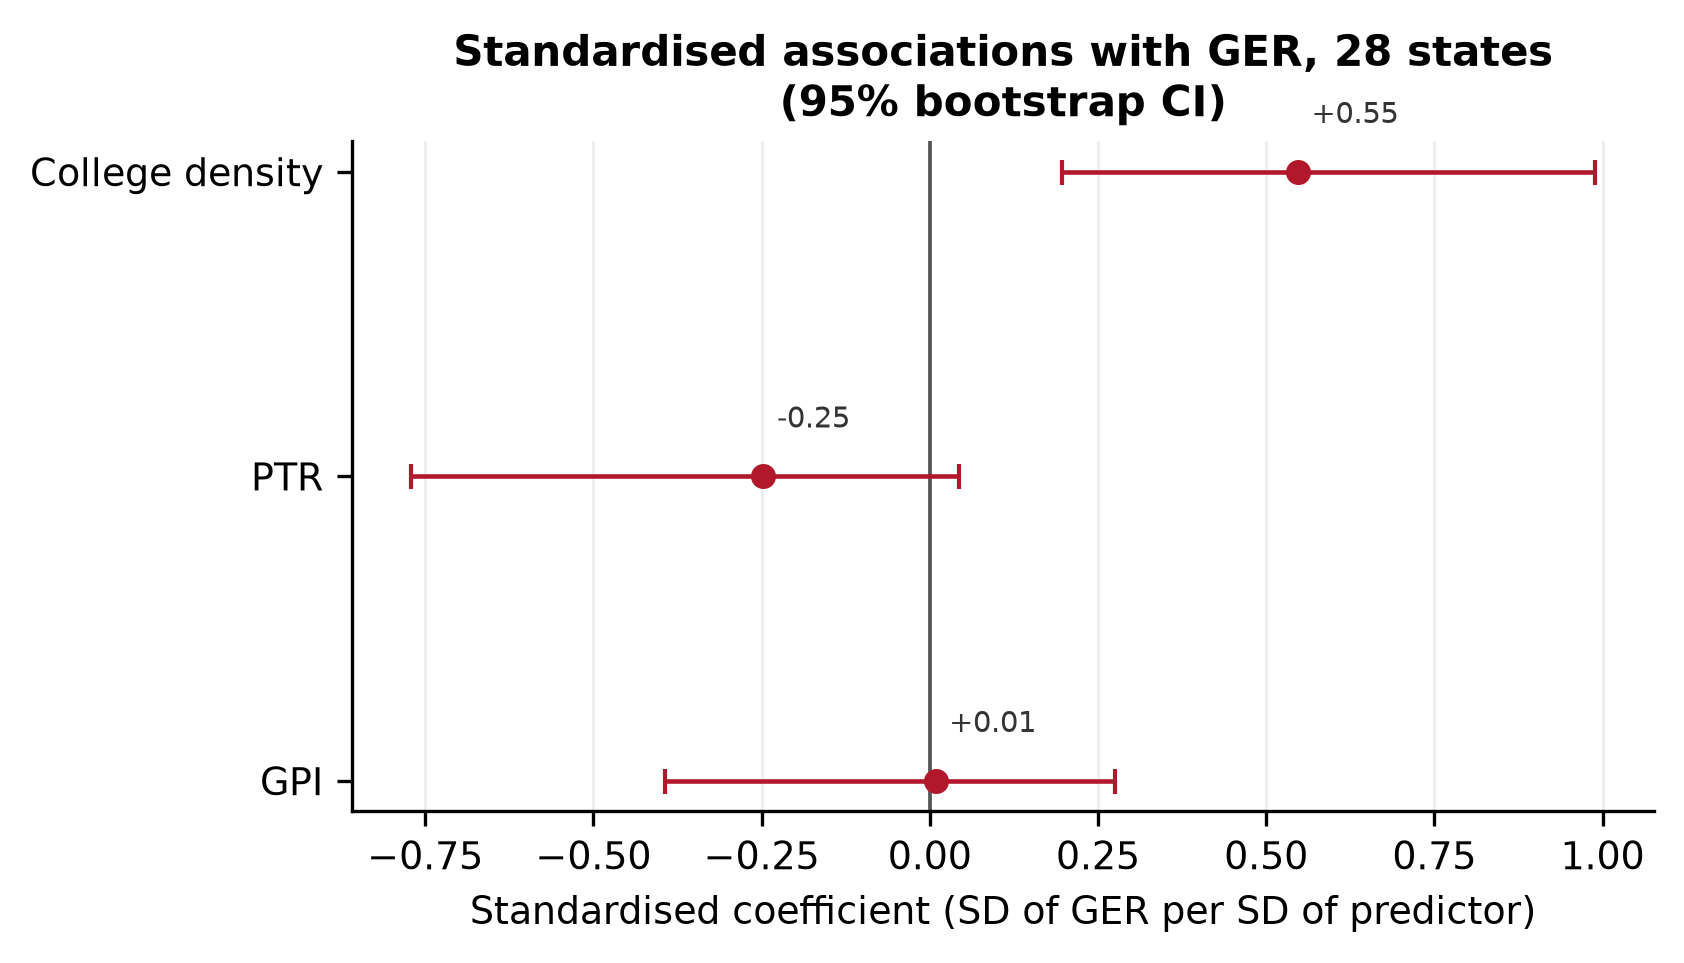
\includegraphics[width=0.9\linewidth]{fig08_coefficients.png}
\caption{Standardised coefficients with 95\% bootstrap confidence intervals, 28 States. Only college density has an interval that excludes zero. Source: \texttt{fig08\_coefficients.png}.}
\label{fig:coefplot}
\end{figure}

\begin{figure}[htbp]
\centering
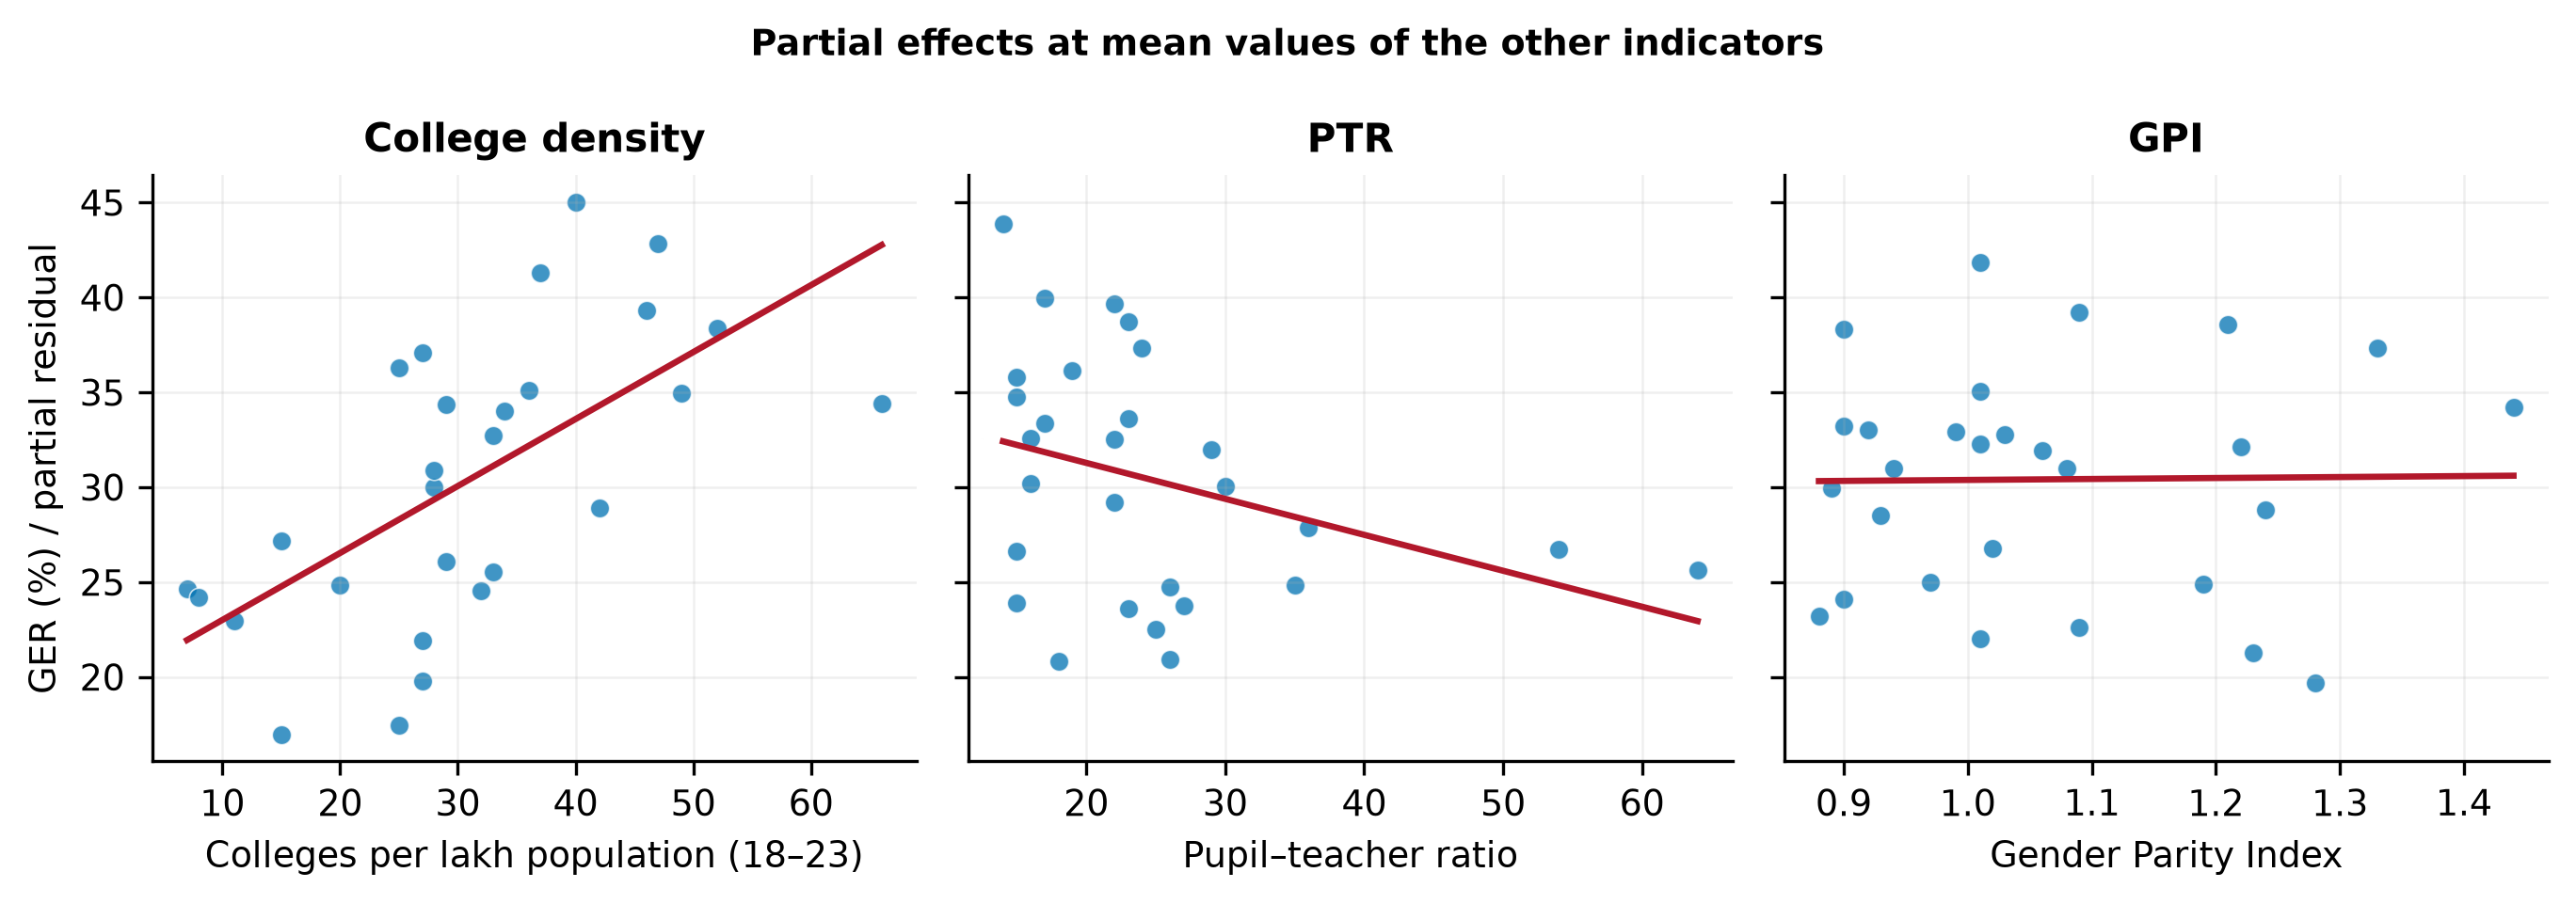
\includegraphics[width=\linewidth]{fig09_partial_effects.png}
\caption{Component-plus-residual partial effects at the mean of the other indicators, 28 States. The density slope is positive; the PTR slope is negative but imprecise; the GPI slope is almost flat. Source: \texttt{fig09\_partial\_effects.png}.}
\label{fig:partial}
\end{figure}

Figure~\ref{fig:coefplot} shows the bootstrap intervals graphically, and Figure~\ref{fig:partial} isolates each partial effect. The density slope is the only one that is clearly separated from zero; the PTR and GPI slopes are consistent with no effect once the other indicators are held constant.

\subsection{Diagnostics and influence}

The OLS residuals are consistent with the classical assumptions (Table~\ref{tab:diagnostics}). Shapiro--Wilk does not reject normality (\(W = 0.969\); \(p = 0.561\)), Breusch--Pagan does not reject homoskedasticity (LM \(= 3.05\); \(p = 0.384\)), and Ramsey RESET does not reject the linear functional form (\(F = 0.021\); \(p = 0.885\)). The condition number is 489, which is moderate for a model with three correlated predictors. No State has a studentised residual above 2 in absolute value.

\begin{table}[htbp]
\centering
\scriptsize
\setlength{\tabcolsep}{3pt}
\caption{Residual diagnostics and influence, OLS three-indicator model, 28 States. The Cook's distance threshold is \(4/n = 0.143\). Source: \texttt{table05\_diagnostics.csv}.}
\label{tab:diagnostics}
\begin{tabular}{@{}p{4.5cm}rp{1.6cm}p{4.1cm}@{}}
\toprule
Diagnostic & Statistic & \(p\)-value & Interpretation \\
\midrule
Shapiro--Wilk (normality) & \(W = 0.969\) & 0.561 & No evidence of non-normality \\
Breusch--Pagan (heterosked.) & LM \(= 3.05\) & 0.384 & No evidence of heteroskedasticity \\
Ramsey RESET (functional form) & \(F = 0.021\) & 0.885 & No evidence of missed nonlinearity \\
Condition number & 489 & --- & Moderate collinearity \\
Maximum Cook's distance & 0.338 & --- & Karnataka; threshold \(4/n = 0.143\) \\
Influential States (Cook's \(D > 4/n\)) & 2 & --- & Karnataka, Nagaland \\
Studentised residuals \(> 2\) in \(|\cdot|\) & 0 & --- & No severe outliers \\
\bottomrule
\end{tabular}
\end{table}

Figure~\ref{fig:residuals} shows the four residual plots; none suggests a systematic departure from the linear specification. Two States are influential. Karnataka has Cook's distance 0.338 and leverage 0.338: it is the highest-density State (66 colleges per lakh) but has a lower GER than the model predicts (residual \(-8.35\)). Nagaland has Cook's distance 0.156 and the largest negative residual (\(-10.85\)). Tamil Nadu has the largest positive residual (\(+11.43\)) but low leverage, so its influence is smaller (Cook's \(D = 0.083\)). Figure~\ref{fig:influence} plots the influence measures, and Figure~\ref{fig:poly} shows the out-of-range behaviour that rules out the polynomial for projection.

\begin{figure}[htbp]
\centering
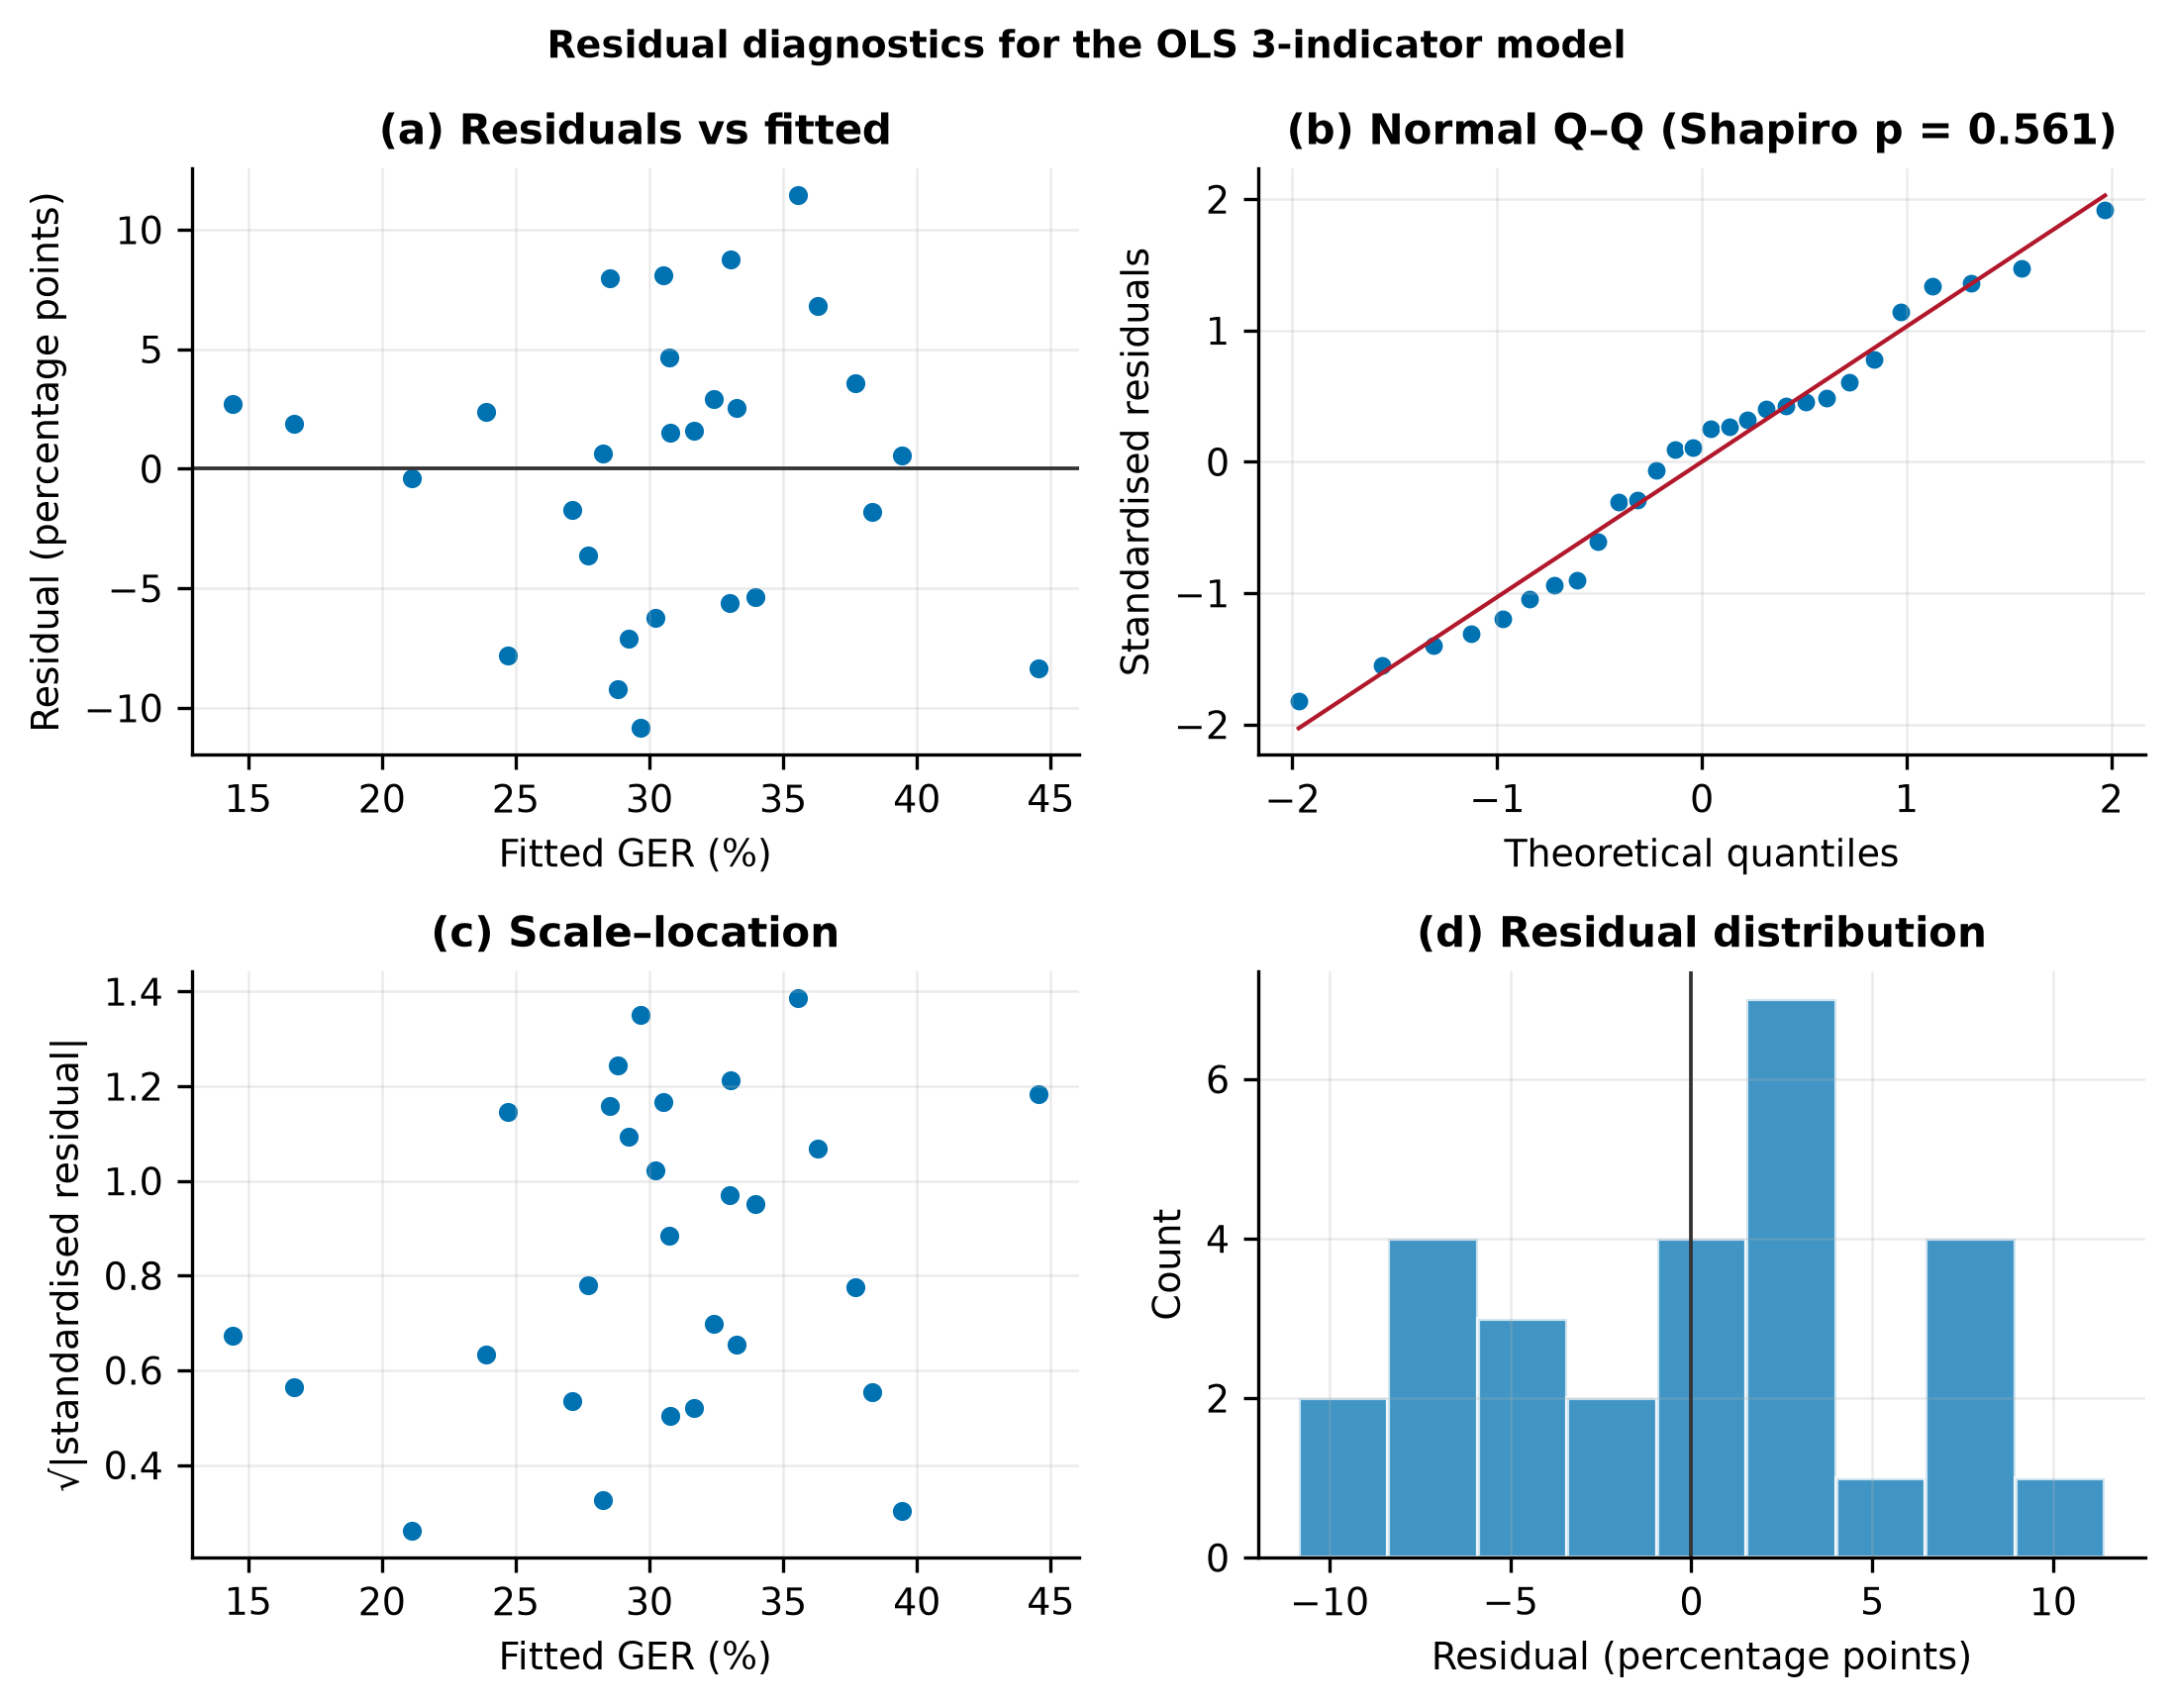
\includegraphics[width=\linewidth]{fig07_residual_diagnostics.png}
\caption{Residual diagnostics for the OLS three-indicator model: residuals versus fitted values, normal Q--Q plot, scale--location plot and residual histogram. Source: \texttt{fig07\_residual\_diagnostics.png}.}
\label{fig:residuals}
\end{figure}

\begin{figure}[htbp]
\centering
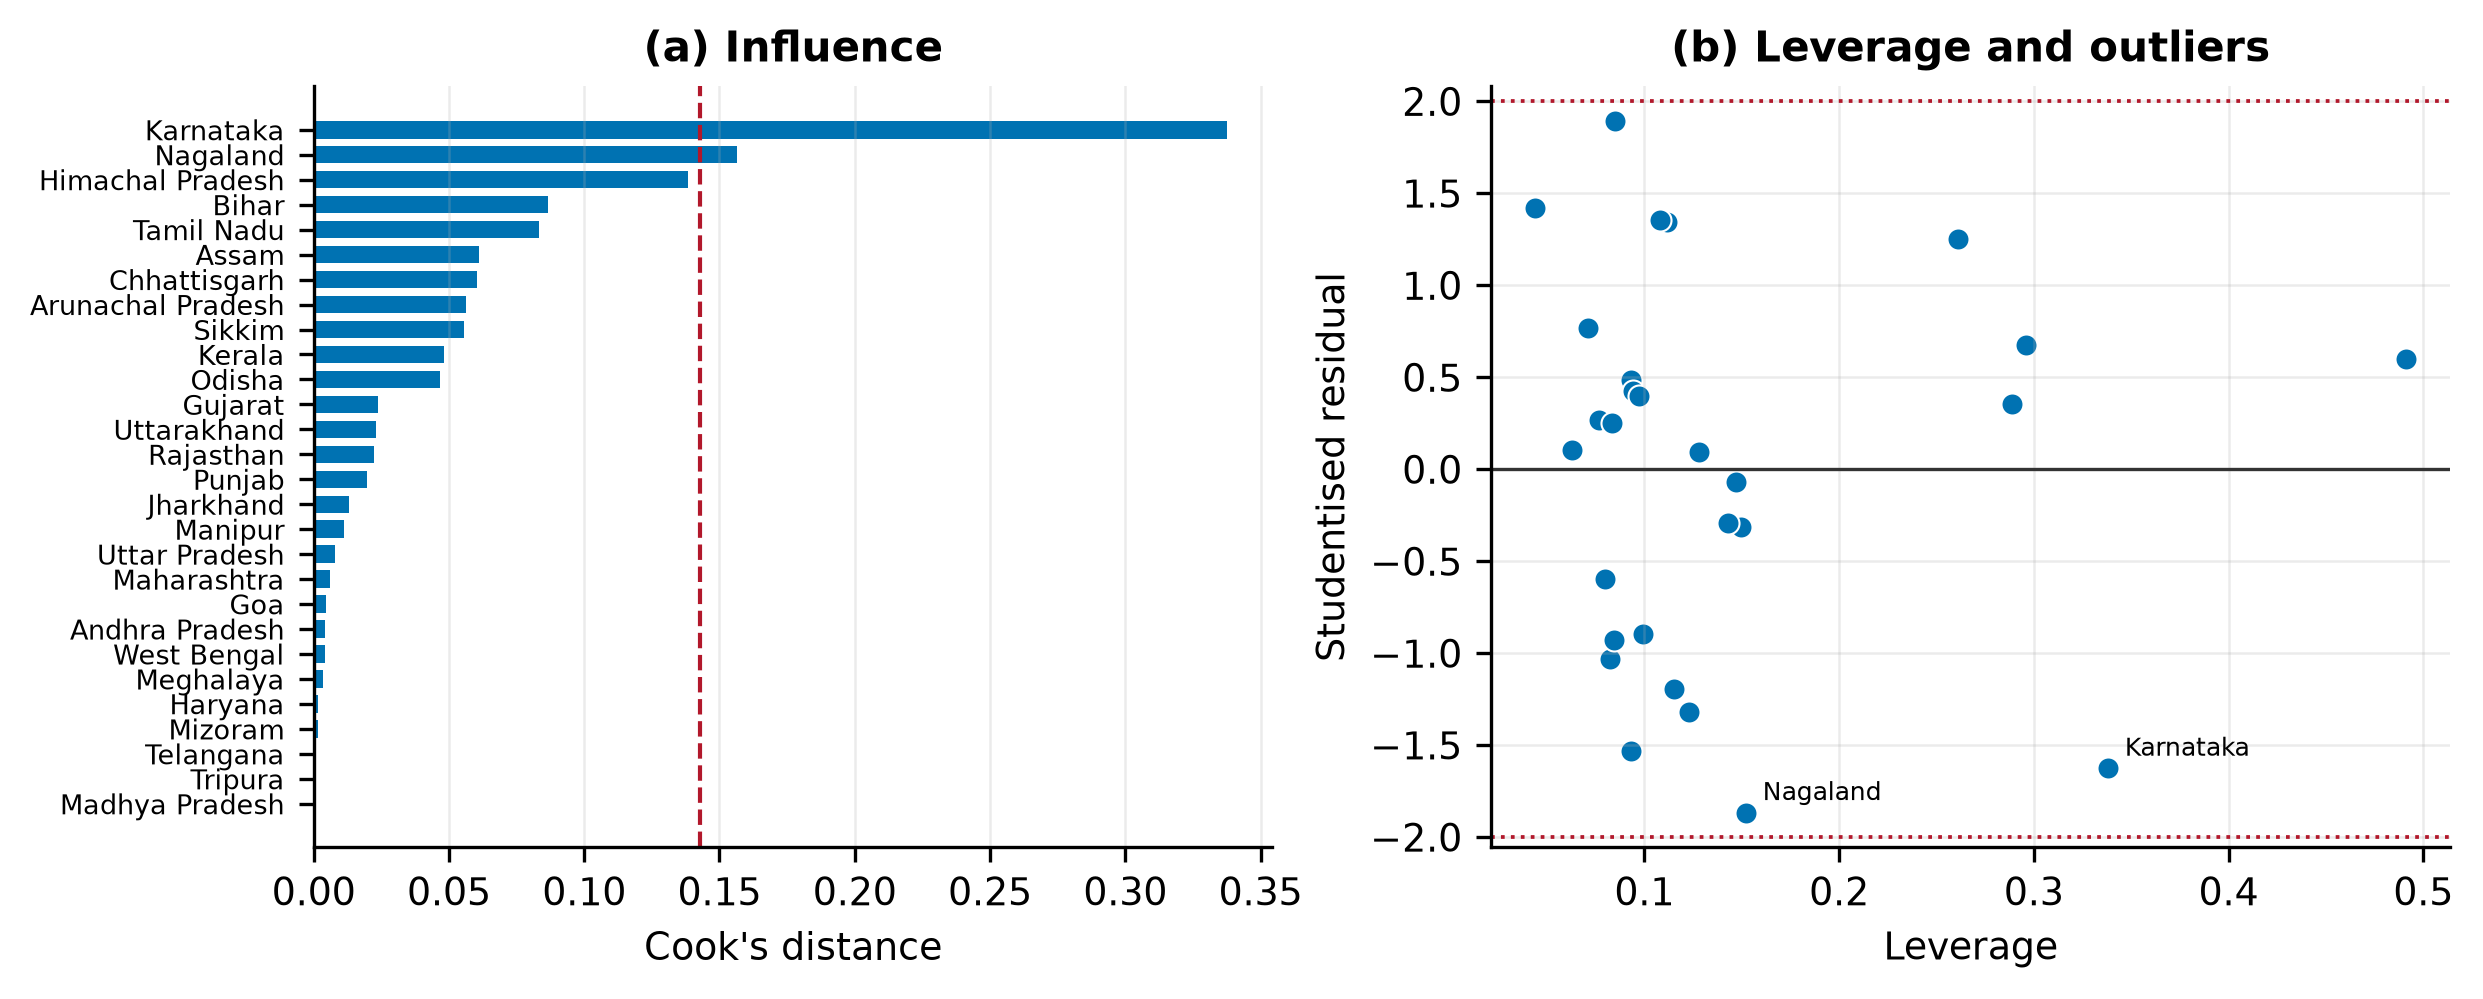
\includegraphics[width=\linewidth]{fig10_influence.png}
\caption{Influence diagnostics: Cook's distance by State and leverage against studentised residual, 28 States. Karnataka and Nagaland exceed the \(4/n\) threshold. Source: \texttt{fig10\_influence.png}.}
\label{fig:influence}
\end{figure}

\begin{figure}[htbp]
\centering
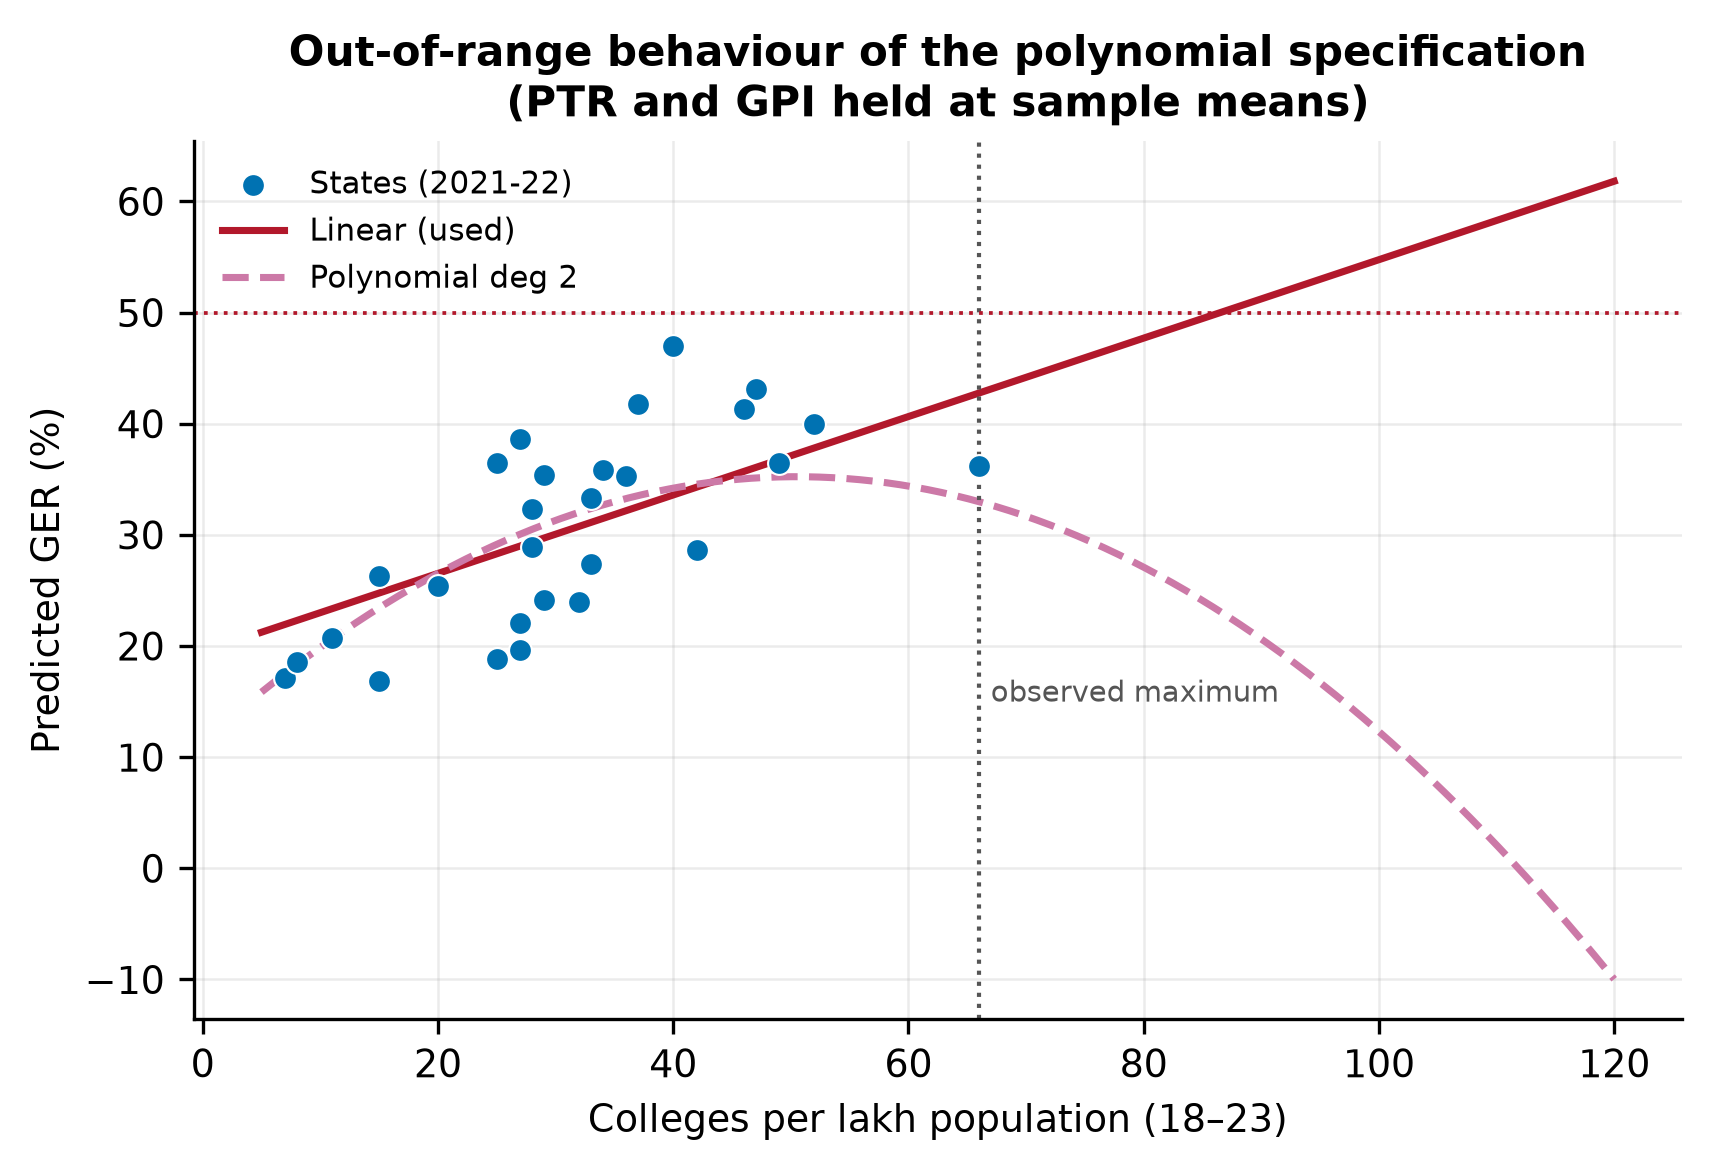
\includegraphics[width=0.9\linewidth]{fig11_polynomial_instability.png}
\caption{Out-of-range behaviour of the polynomial specification. The degree-2 fit turns downward beyond the observed density range and eventually predicts negative GER, whereas the linear fit remains monotone. This is why the polynomial is a predictive benchmark, not the projection model. Source: \texttt{fig11\_polynomial\_instability.png}.}
\label{fig:poly}
\end{figure}

\subsection{Panel and sensitivity checks}\label{sec:panel}

Table~\ref{tab:sensitivity} reports the panel and leave-out checks. The density association is stable: 0.355 with year fixed effects, 0.398 with State and year fixed effects, and 0.752 in first differences. The first-difference estimate is larger, which suggests that within-State expansion is associated with larger GER gains than the cross-section alone implies. The short panel and measurement error caution against over-interpretation, but the sign and order of magnitude are consistent.

\begin{table}[htbp]
\centering
\caption{Panel, leave-out and UT-inclusive specifications. Panel rows use State-clustered standard errors; cross-section HC3 \(p\)-values are reported in Table~\ref{tab:coefficients}. The Sikkim-excluded row checks whether the common trend depends on one anomalous series. Source: \texttt{table07\_sensitivity.csv}.}
\label{tab:sensitivity}
\resizebox{\textwidth}{!}{%
\begin{tabular}{@{}lrrrrr@{}}
\toprule
Specification & \(n\) & Density coef. & PTR coef. & GPI coef. & \(R^2\) / LOOCV \(R^2\) \\
\midrule
Cross-section OLS & 28 & 0.353 & $-0.189$ & 0.508 & \(R^2 = 0.543\) \\
Panel, year FE & 140 & 0.355 & $-0.215$ & $-0.846$ & \(R^2 = 0.480\) \\
Panel, year FE excluding Sikkim & 135 & 0.416 & $-0.107$ & $+2.287$ & \(R^2 = 0.585\) \\
Panel, State + year FE & 140 & 0.398 & $+0.343$ & $-26.98$ & \(R^2 = 0.945\) \\
First differences & 112 & 0.752 & $+0.146$ & $-28.39$ & \(R^2 = 0.395\) \\
OLS excluding Karnataka & 27 & 0.474 & $-0.136$ & $-1.245$ & \(R^2 = 0.586\); LOOCV \(R^2 = 0.457\) \\
OLS excluding Karnataka + Bihar & 26 & 0.461 & $-0.208$ & $-1.564$ & \(R^2 = 0.555\); LOOCV \(R^2 = 0.392\) \\
All 35 units, core & 35 & --- & --- & --- & LOOCV \(R^2 = 0.158\) \\
All 35 units, core + UT dummy & 35 & --- & --- & --- & LOOCV \(R^2 = 0.180\) \\
\bottomrule
\end{tabular}}
\end{table}

PTR is not robust. It is \(-0.215\) in the year fixed-effects model but \(+0.343\) with State fixed effects and \(+0.146\) in first differences. The sign flip is exactly what one would expect from reverse causality and from the mechanical relationship between PTR and enrolment. A State that expands enrolment without matching teacher hiring will raise its PTR; a State that hires teachers without expanding enrolment will lower it. The cross-sectional negative correlation is therefore not a credible estimate of the effect of teacher supply.

GPI is also unstable and imprecisely estimated. The large negative coefficients in the State fixed-effects and first-difference models reflect limited within-State variation and collinearity, not a credible policy effect. The aggregate GER is simply not a good outcome for identifying gender-specific constraints.

The common annual trend from the year fixed-effects model is 0.866 GER points per year (SE 0.174). Over 14 years this is about 12.1 points, with a 95\% interval of roughly 7.2 to 17.0 points. This trend is a key input to the projection and a major source of uncertainty. It is an average from a short, Covid-affected panel; it may not continue for 14 years, and it is unlikely to be the same in every State.

One series needs a caveat. Sikkim reports a GER of 66.9\% in 2019-20, having reported 48.1\% the year before and 39.9\% the year after. A 27-point fall in one year is not a plausible change in participation; it is almost certainly a change in how the State reported enrolment or population. Sikkim is retained in the primary estimates because deleting a State for looking unusual is a judgement that should be made transparently rather than silently, and because the alternative would be to drop a genuine data point. As a check, the year fixed-effects model is re-estimated without Sikkim: the density coefficient rises to 0.416, the common trend falls only to 0.845 (SE 0.161), and \(R^2\) rises from 0.480 to 0.585. The trend used in the projection, 0.866, is therefore not an artefact of the Sikkim series, and the density result is, if anything, stronger without it. Figure~\ref{fig:trajectories} annotates the observation.

The leave-out checks strengthen the density result. Excluding Karnataka raises the density coefficient to 0.474 (\(p = 0.001\)) and the in-sample \(R^2\) to 0.586. Excluding Karnataka and Bihar gives 0.461 (\(p = 0.002\)) and \(R^2 = 0.555\). The coefficient is larger without Karnataka because Karnataka is a high-density, low-GER outlier that pulls the slope down. The result does not depend on one or two States.

The UT-inclusive models perform much worse out of sample: LOOCV \(R^2\) is 0.158 without a UT dummy and 0.180 with one, and RMSE is about 11.2--11.4. This confirms that UTs are not exchangeable with States and justifies the primary sample choice.

\subsection{Projections to 2035-36}

Table~\ref{tab:scenariosummary} summarises the three scenarios. Under the reference scenario (S2), 13 of 28 States reach 50\% by 2035-36. Under the damped scenario (S1), only three do. The reform scenario (S3) also produces 13 crossings: PTR and GPI reforms raise the mean projection by about 1.2 points, but they do not move any additional State across the line.

\begin{table}[htbp]
\centering
\caption{Scenario summary, 28 States, 2035-36. Point estimates and probabilities come from 2,000 bootstrap draws; the last column counts States by \(P(\GER \ge 50\%)\) as on track / at risk / off track. State detail is in \texttt{table06\_projections\_2035.csv}. Source: \texttt{table09\_scenario\_summary.csv}.}
\label{tab:scenariosummary}
\resizebox{\textwidth}{!}{%
\begin{tabular}{@{}lrrrrrrl@{}}
\toprule
Scenario & Point \(\ge 50\%\) & \(P(\GER \ge 50\%) \ge 0.5\) & Mean & Median & Min & Max & On / at risk / off \\
\midrule
S1 Damped & 3 & 3 & 38.2 & 40.7 & 23.2 & 56.2 & 3 / 6 / 19 \\
S2 Recent trend (reference) & 13 & 13 & 45.8 & 49.5 & 28.5 & 65.3 & 13 / 3 / 12 \\
S3 NEP reform & 13 & 13 & 47.0 & 49.7 & 28.5 & 65.3 & 13 / 4 / 11 \\
\bottomrule
\end{tabular}}
\end{table}

The 13 States reaching 50\% under S2 are Tamil Nadu (65.3), Himachal Pradesh (57.7), Uttarakhand (53.9), Kerala (55.9), Telangana (53.4), Sikkim (56.9), Arunachal Pradesh (56.0), Karnataka (60.3), Goa (50.4), Manipur (51.2), Maharashtra (51.1), Mizoram (50.6) and Rajasthan (51.8). Three are at risk rather than off track: Andhra Pradesh (49.9; \(P = 0.49\)), Haryana (49.1; \(P = 0.47\)) and Madhya Pradesh (46.0; \(P = 0.29\)). The remaining 12 are off track: Punjab (39.5), West Bengal (42.1), Meghalaya (40.0), Uttar Pradesh (37.5), Gujarat (38.6), Odisha (39.2), Tripura (31.6), Chhattisgarh (35.4), Nagaland (28.5), Jharkhand (30.7), Bihar (29.2) and Assam (30.3).

\begin{figure}[htbp]
\centering
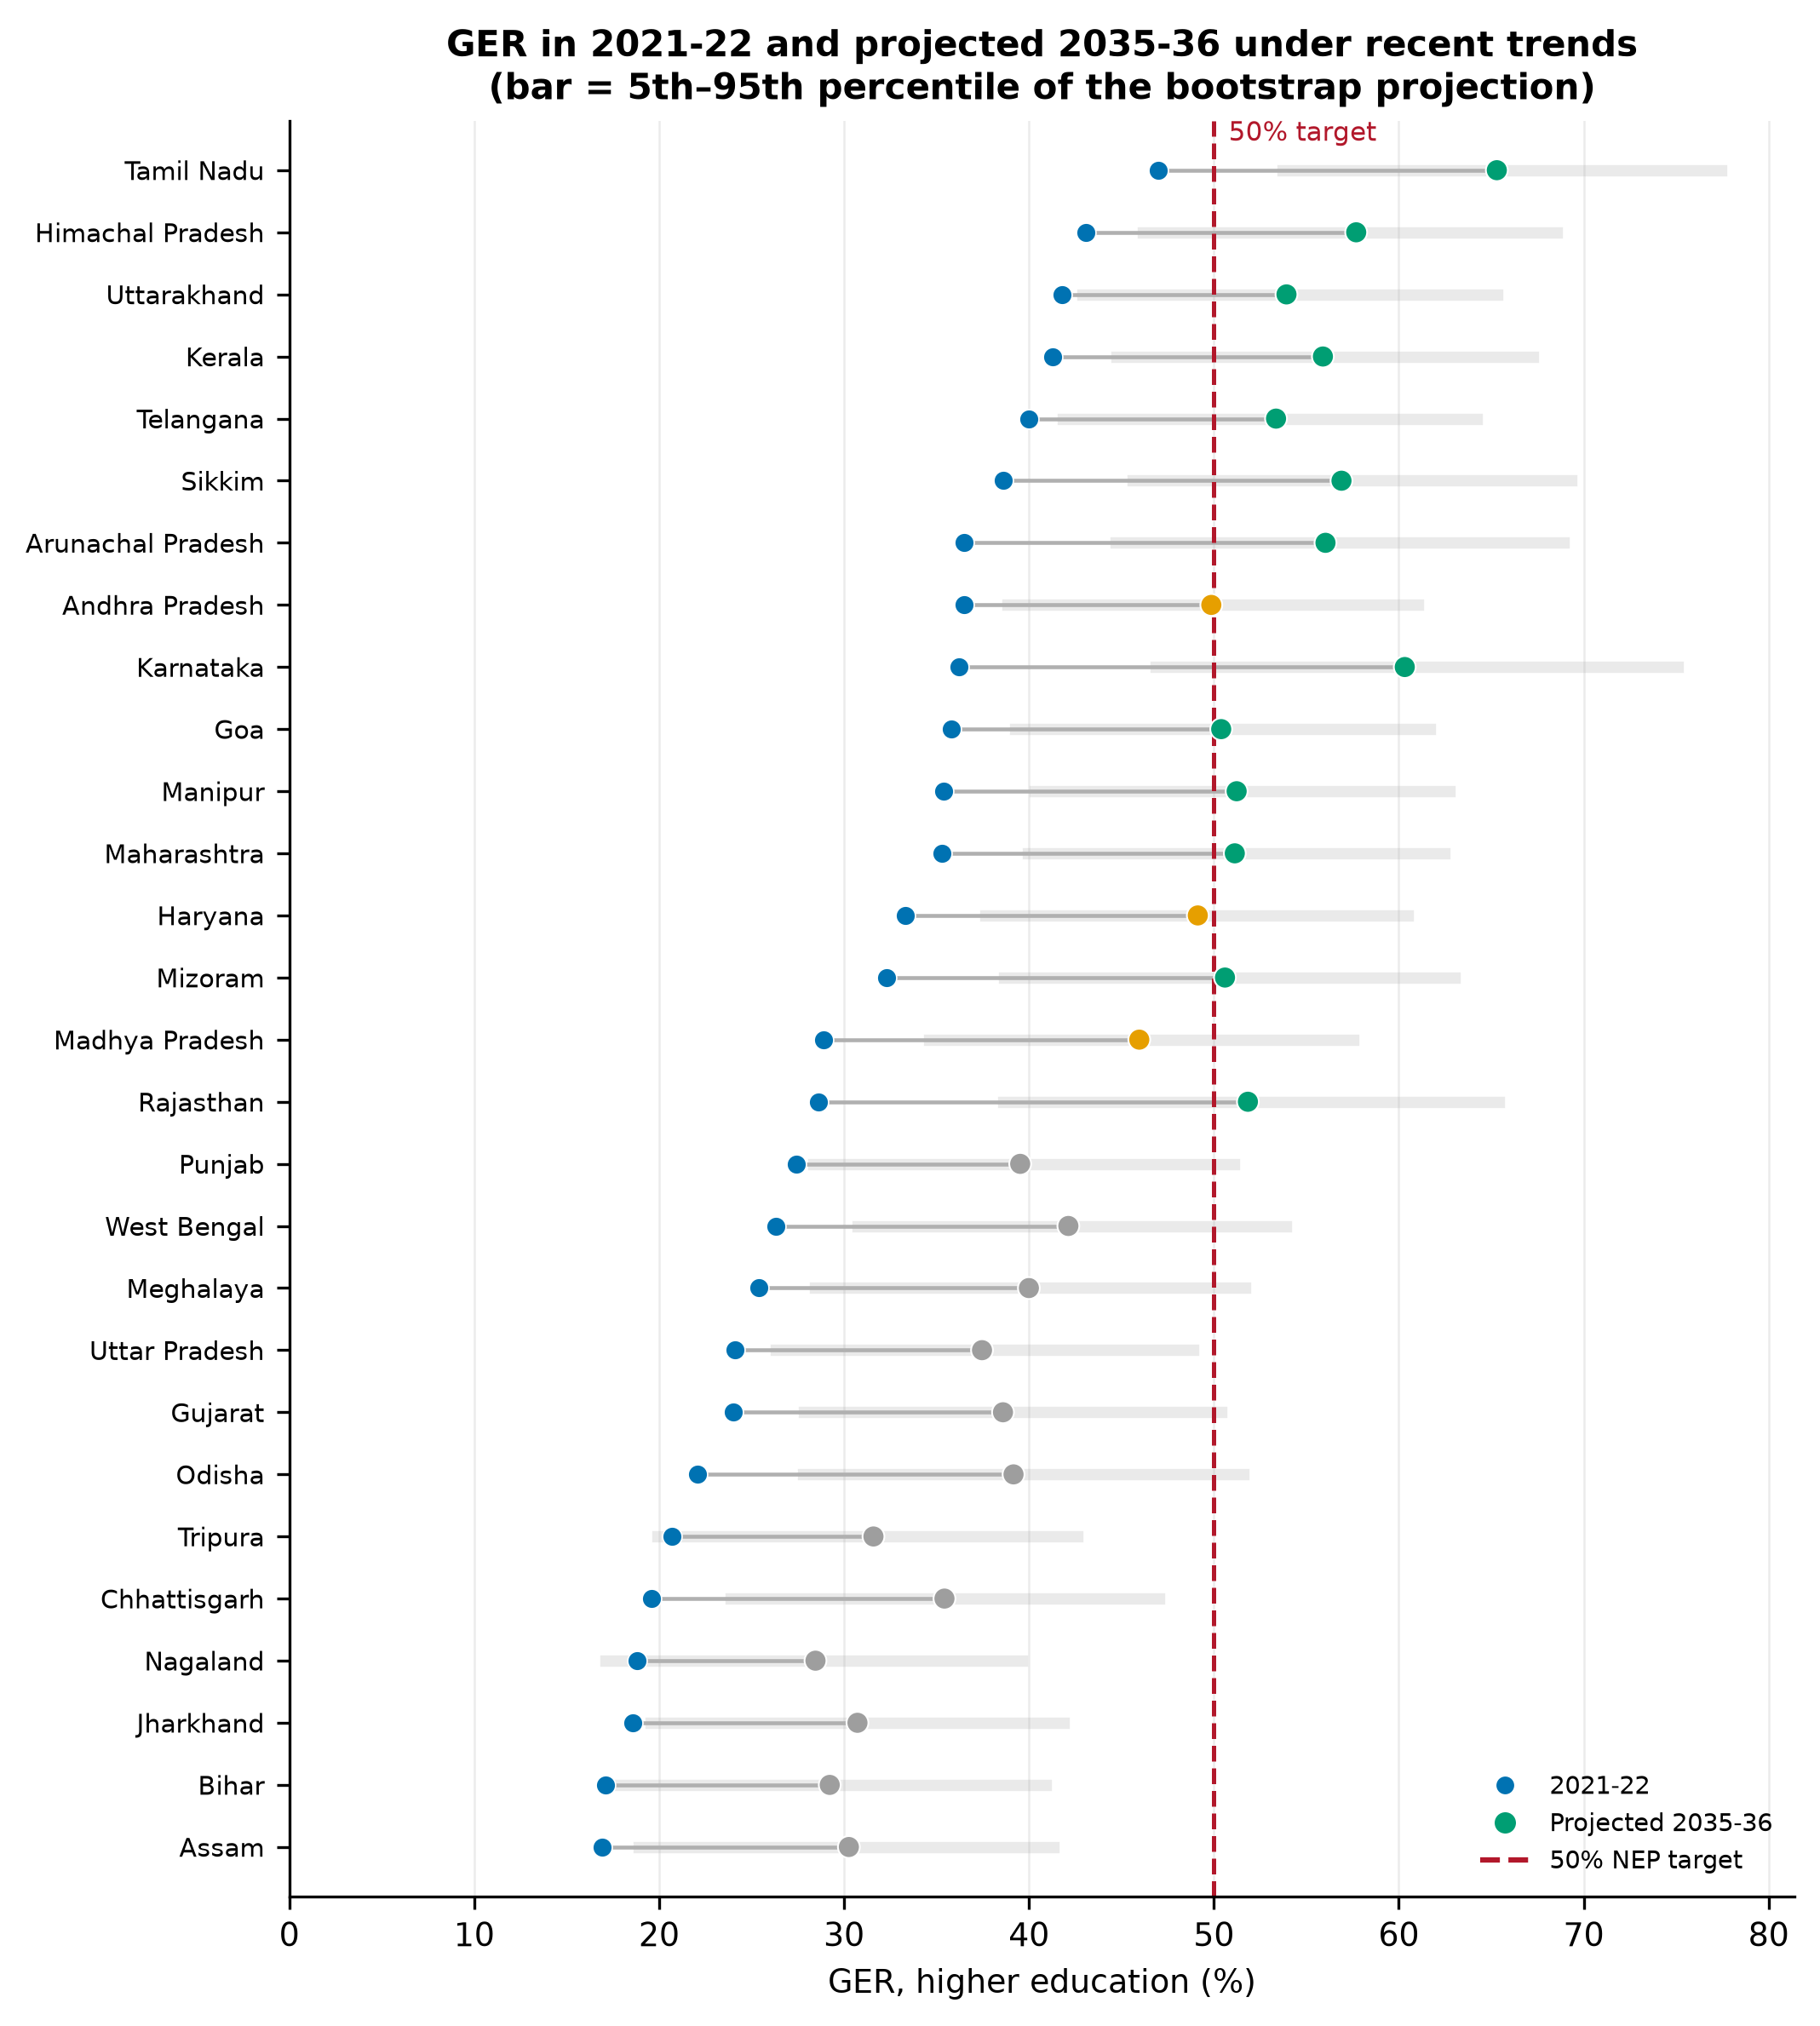
\includegraphics[width=\linewidth]{fig12_projection_dumbbell.png}
\caption{Observed GER in 2021-22 and projected GER in 2035-36 under recent trends, 28 States. Bars show the 5th--95th percentile bootstrap interval; the dashed line is the 50\% target. Source: \texttt{fig12\_projection\_dumbbell.png}.}
\label{fig:dumbbell}
\end{figure}

\begin{figure}[htbp]
\centering
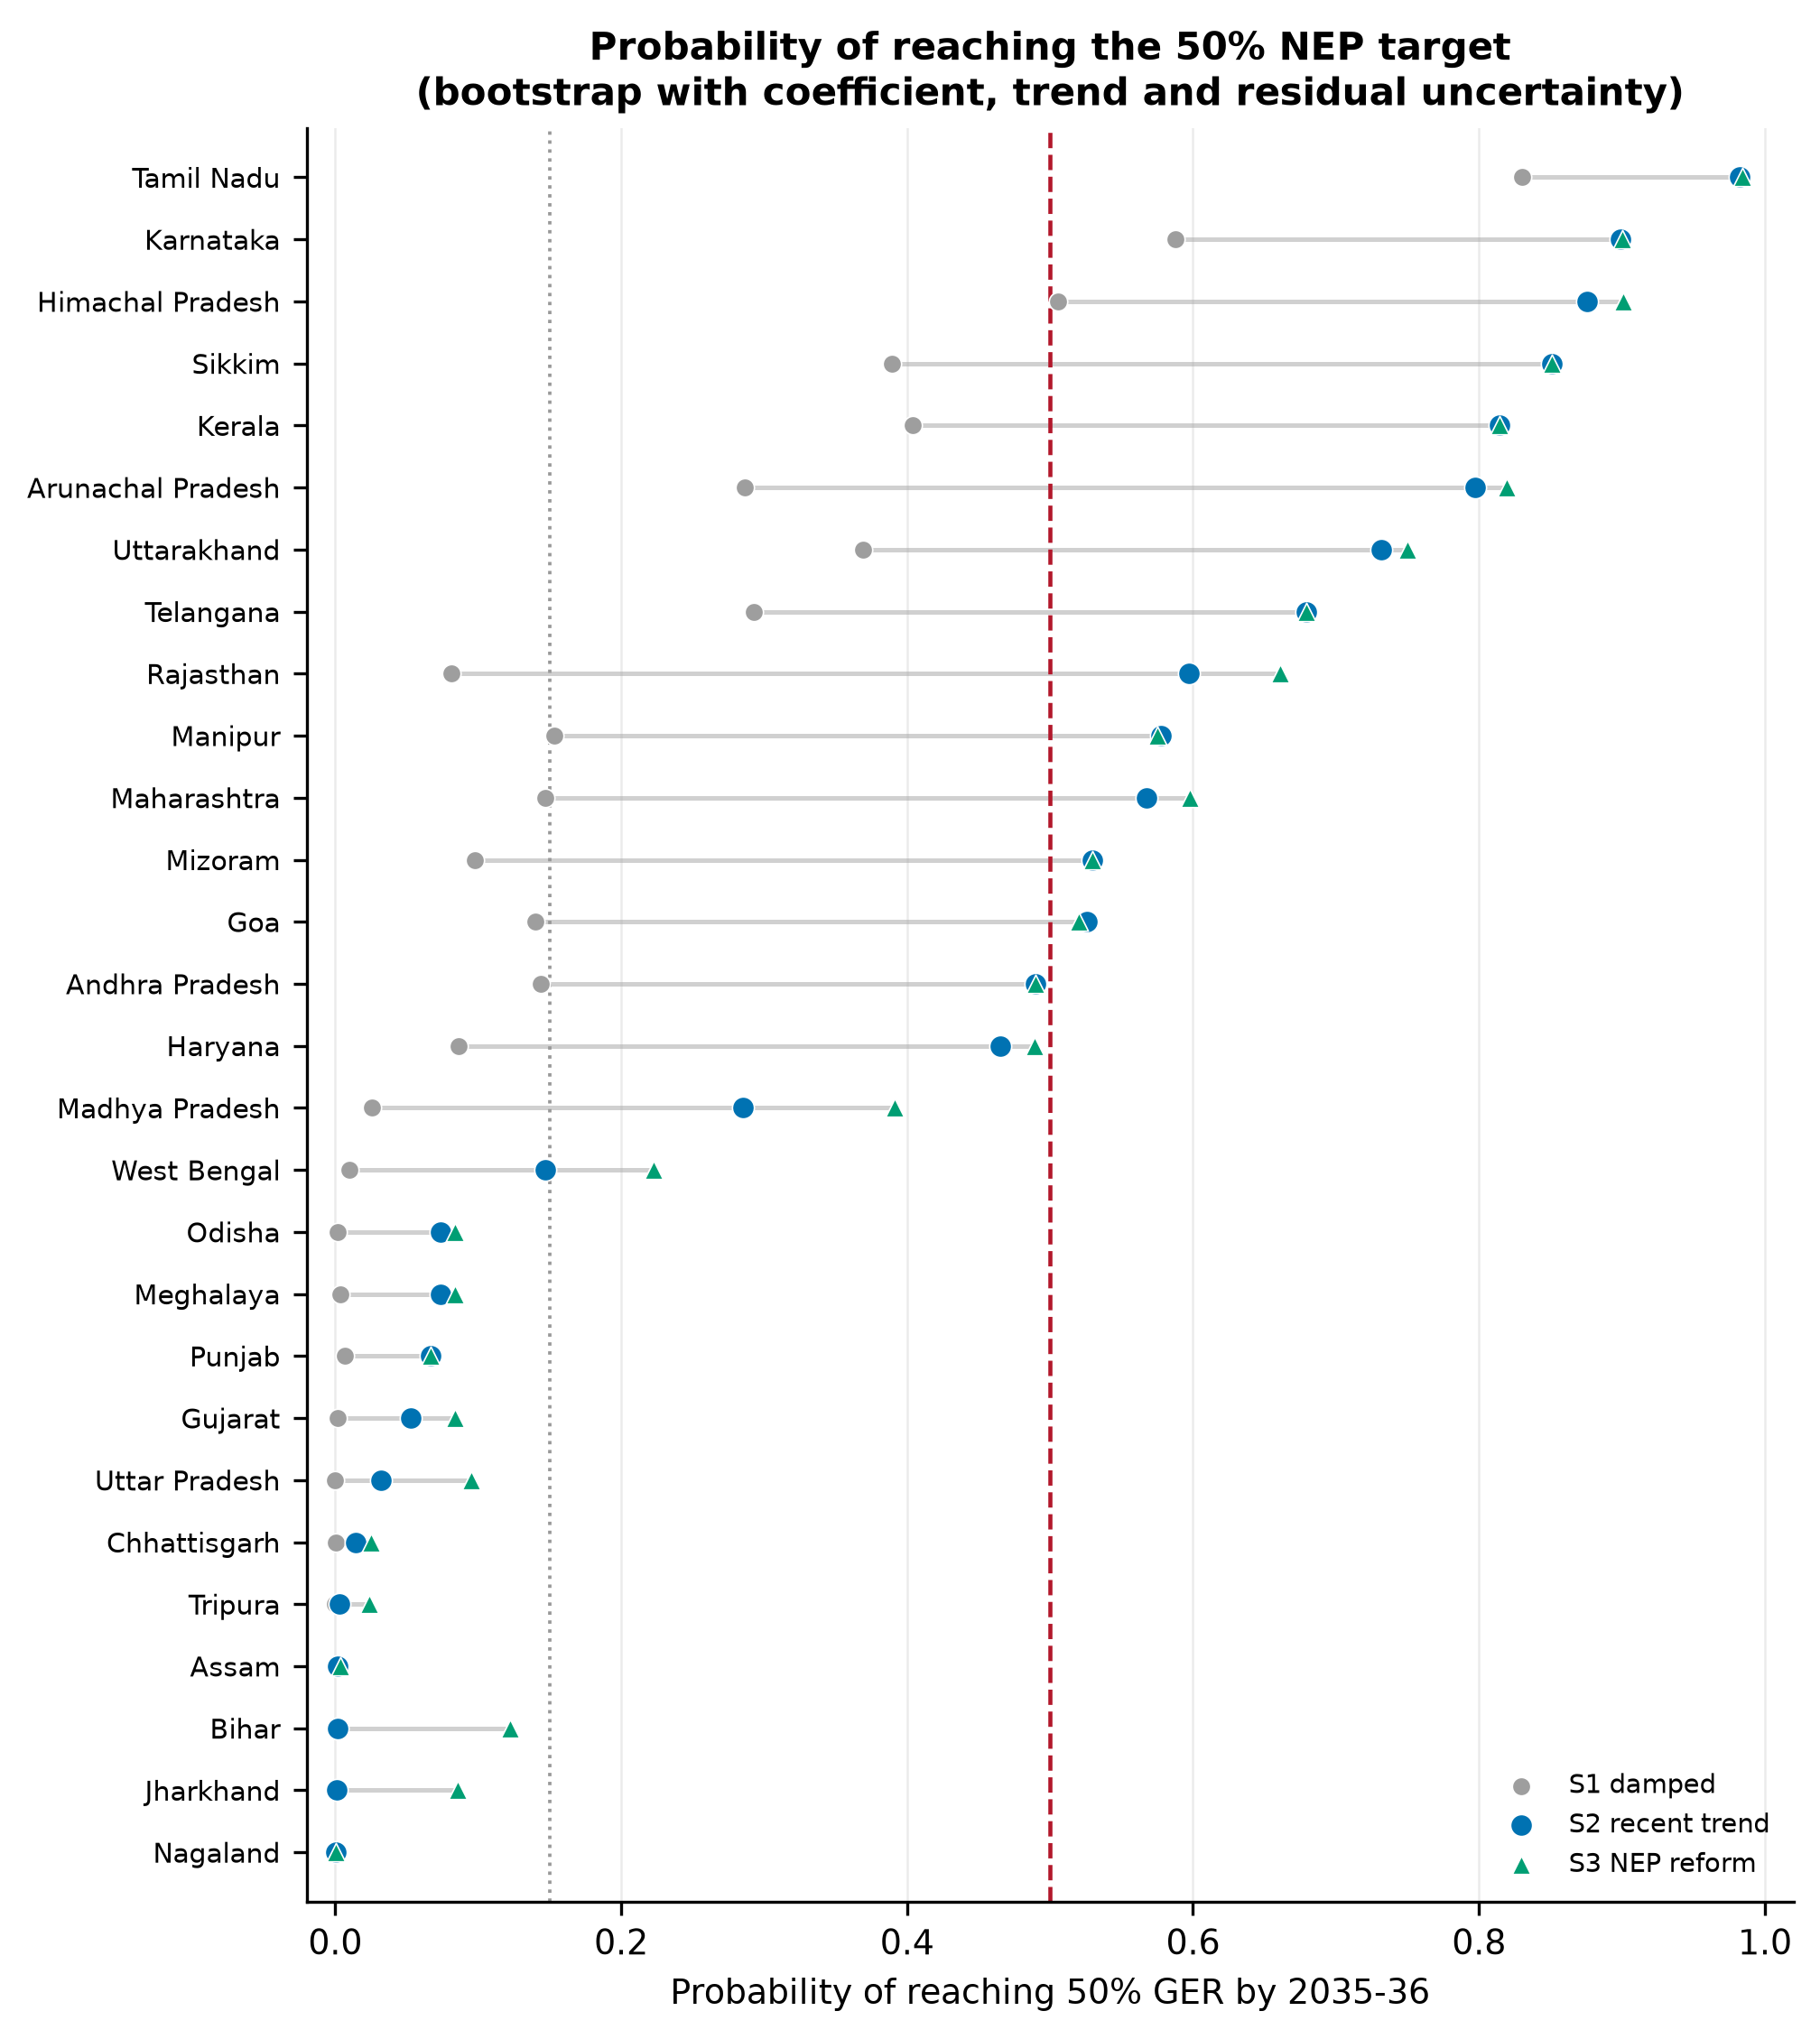
\includegraphics[width=\linewidth]{fig13_probability_reaching_50.png}
\caption{Probability of reaching 50\% by 2035-36 under the three scenarios, 28 States. The 0.5 and 0.15 lines mark the on-track and at-risk thresholds. Source: \texttt{fig13\_probability\_reaching\_50.png}.}
\label{fig:prob50}
\end{figure}

\begin{figure}[htbp]
\centering
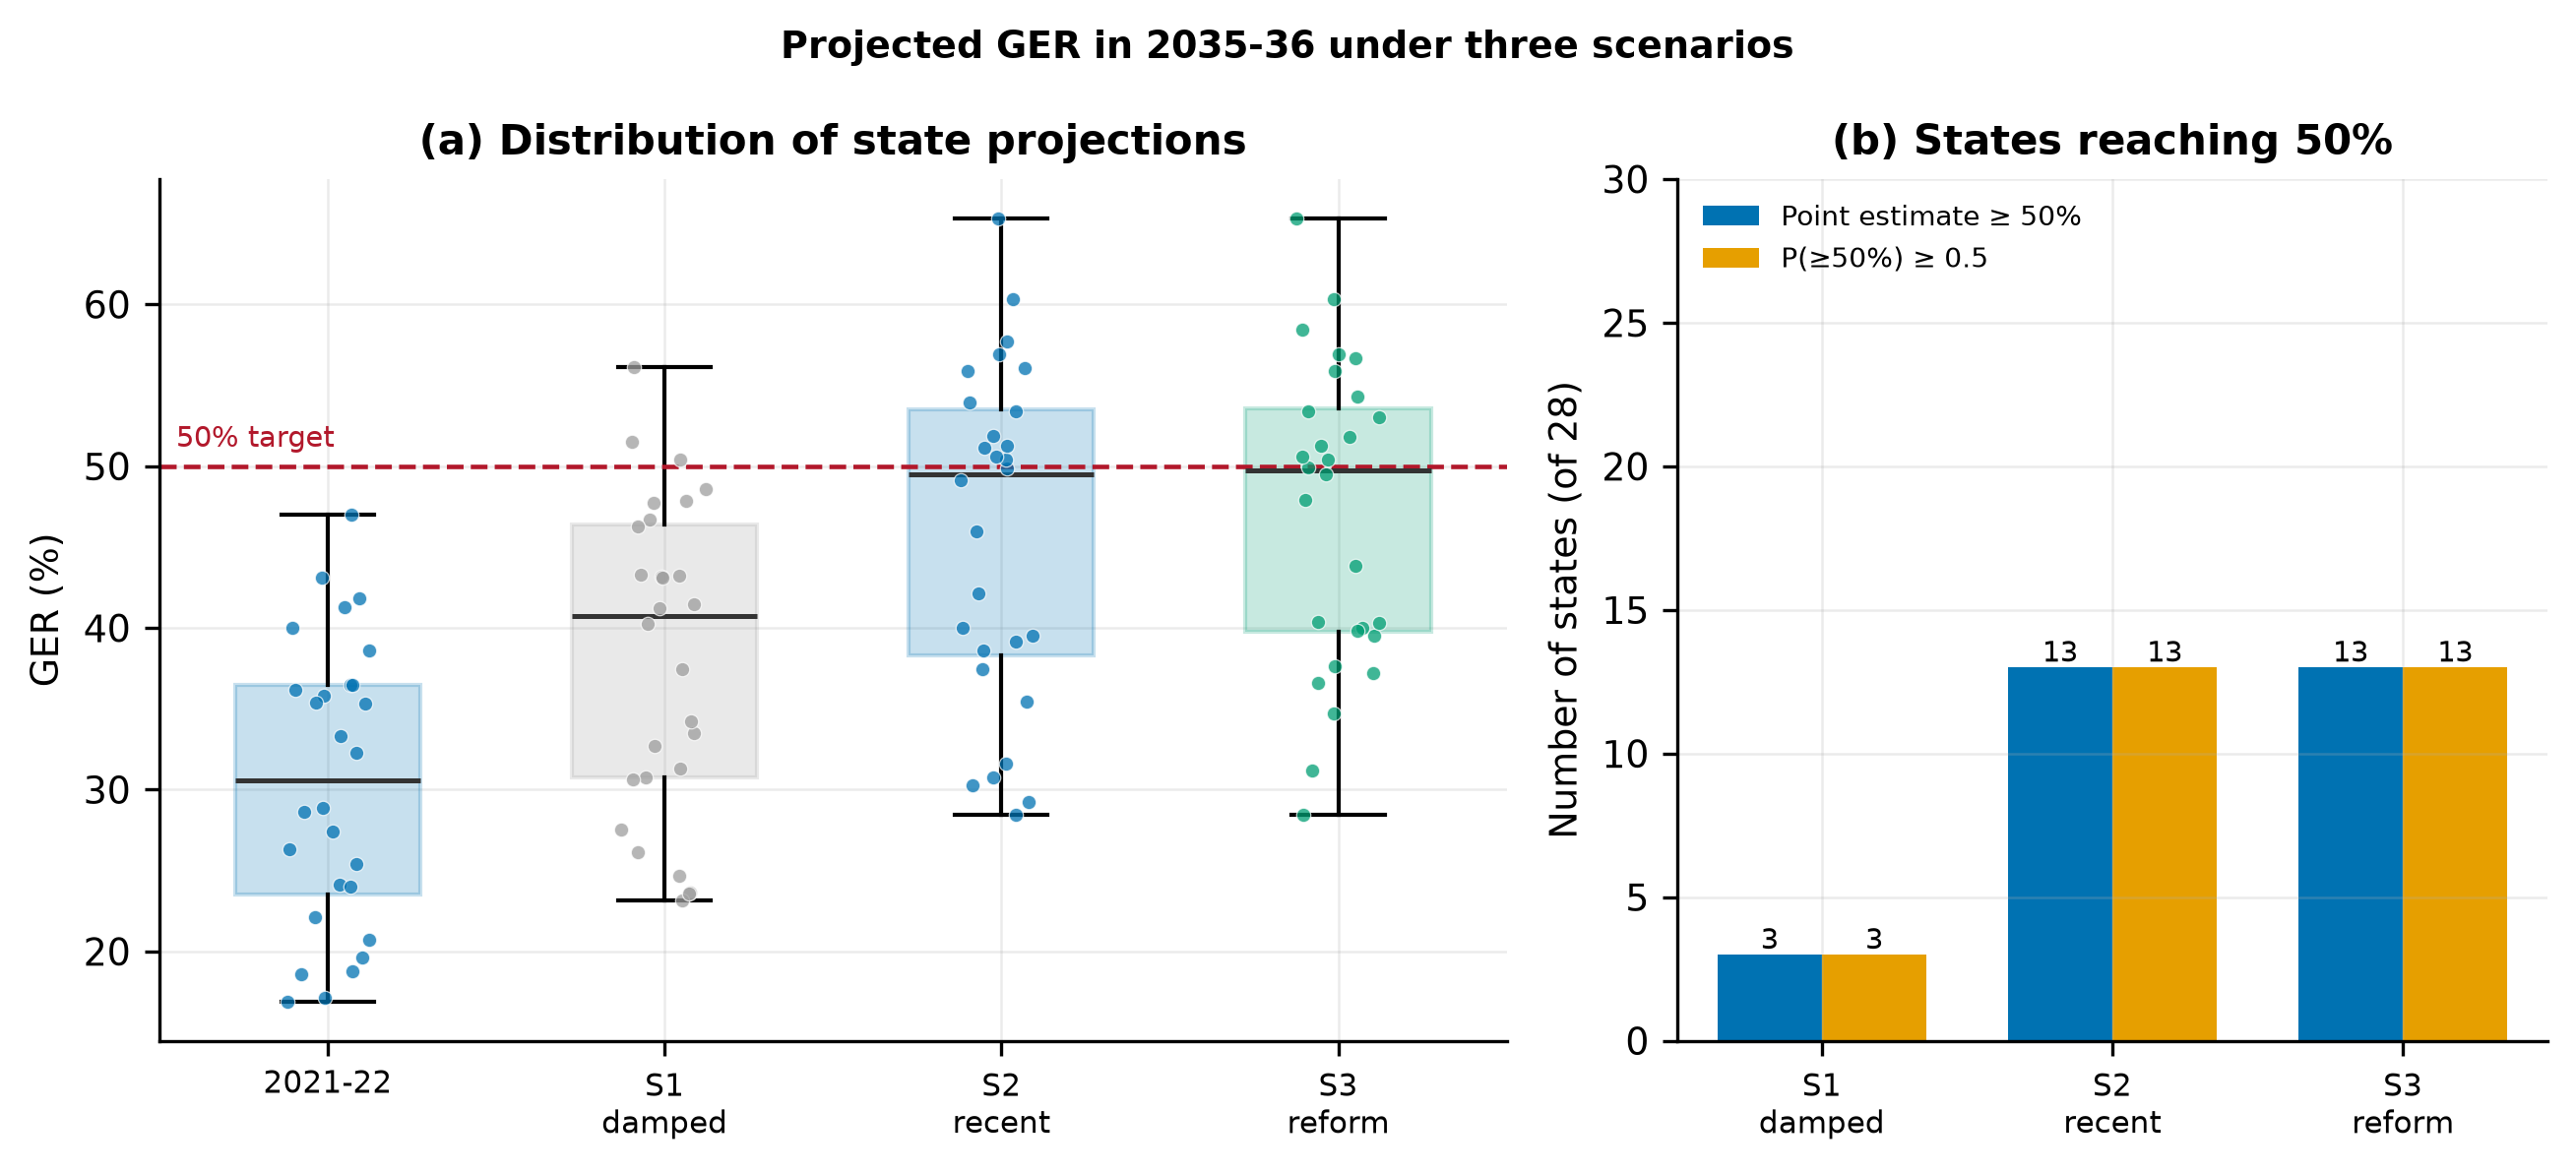
\includegraphics[width=\linewidth]{fig14_scenario_distributions.png}
\caption{Distribution of State projections and the number of States reaching 50\% under each scenario, 28 States. Source: \texttt{fig14\_scenario\_distributions.png}.}
\label{fig:scenariodist}
\end{figure}

Figure~\ref{fig:dumbbell} shows the State-level change and its uncertainty, Figure~\ref{fig:prob50} ranks States by the probability of crossing 50\%, and Figure~\ref{fig:scenariodist} compares the three scenario distributions. The uncertainty is large. For Tamil Nadu, the 5th--95th percentile interval is 53.7 to 77.4; for Bihar it is 17.9 to 40.9. The width reflects three sources: coefficient uncertainty (especially the density coefficient), trend uncertainty (0.866 $\pm$ 0.174 per year) and State-level residual variation (SD \(= 6.31\)). The probability ranking is therefore more informative than a single point forecast.

The population-weighted check is the central result. Using the implied 18--23 population as weights, the 28-State GER rises from 28.0\% in 2021-22 to 35.9\% under S1, 43.5\% under S2 and 45.7\% under S3 in 2035-36. Even the reference scenario leaves the population-weighted GER 6.5 points below the NEP target, and 68.6\% of the 18--23 population lives in States projected below 50\%. The unweighted count of 13 States overstates national progress because the States that are off track are the populous ones.

\subsection{What would it take? Required density}

Table~\ref{tab:required} reports the model-implied college density required by 2035-36 under S2, computed from~\eqref{eq:required} for the ten largest gaps. The required annual changes are far above the observed 2017-22 changes in the low-density States. Bihar would need \(+4.2\) colleges per lakh per year, against an observed change of zero; Uttar Pradesh \(+2.8\) against \(+0.25\); Assam \(+4.2\) against \(+0.25\); Jharkhand \(+3.9\) against zero. Nagaland has the largest gap in college density terms (61.1), but the smallest implied population, so the indicative college requirement is only about 170.

\begin{table}[htbp]
\centering
\caption{Model-implied college density required by 2035-36 under S2, ten largest gaps. \(D_{s,2021}\) is observed college density, \(D_{s,2035}\) is the S2 college density, and \(D_s^{\text{req}}\) is the college density from~\eqref{eq:required} that would deliver 50\% under the model. ``Extra colleges'' multiplies the density gap by the implied 18--23 population; it is an illustration, not a costing. Source: \texttt{table08\_required\_density.csv}.}
\label{tab:required}
\resizebox{\textwidth}{!}{%
\begin{tabular}{@{}lrrrrrrr@{}}
\toprule
State & \(D_{s,2021}\) & \(D_{s,2035}\) & \(D_s^{\text{req}}\) & Gap & Req.\ annual & Obs.\ annual & Extra colleges \\
\midrule
Nagaland & 25 & 18.0 & 79.1 & 61.1 & +3.86 & $-0.50$ & 169 \\
Bihar & 7 & 7.0 & 65.9 & 58.9 & +4.20 & 0.00 & 9,184 \\
Assam & 15 & 18.5 & 74.4 & 55.9 & +4.25 & +0.25 & 2,264 \\
Jharkhand & 8 & 8.0 & 62.6 & 54.6 & +3.90 & 0.00 & 2,499 \\
Tripura & 11 & 7.5 & 59.7 & 52.2 & +3.48 & $-0.25$ & 256 \\
Chhattisgarh & 27 & 37.5 & 78.8 & 41.3 & +3.70 & +0.75 & 1,402 \\
Uttar Pradesh & 29 & 32.5 & 68.0 & 35.5 & +2.79 & +0.25 & 10,262 \\
Gujarat & 32 & 39.0 & 71.3 & 32.3 & +2.81 & +0.50 & 2,419 \\
Odisha & 27 & 41.0 & 71.7 & 30.7 & +3.19 & +1.00 & 1,478 \\
Punjab & 33 & 33.0 & 62.7 & 29.7 & +2.12 & 0.00 & 939 \\
\bottomrule
\end{tabular}}
\end{table}

\begin{figure}[htbp]
\centering
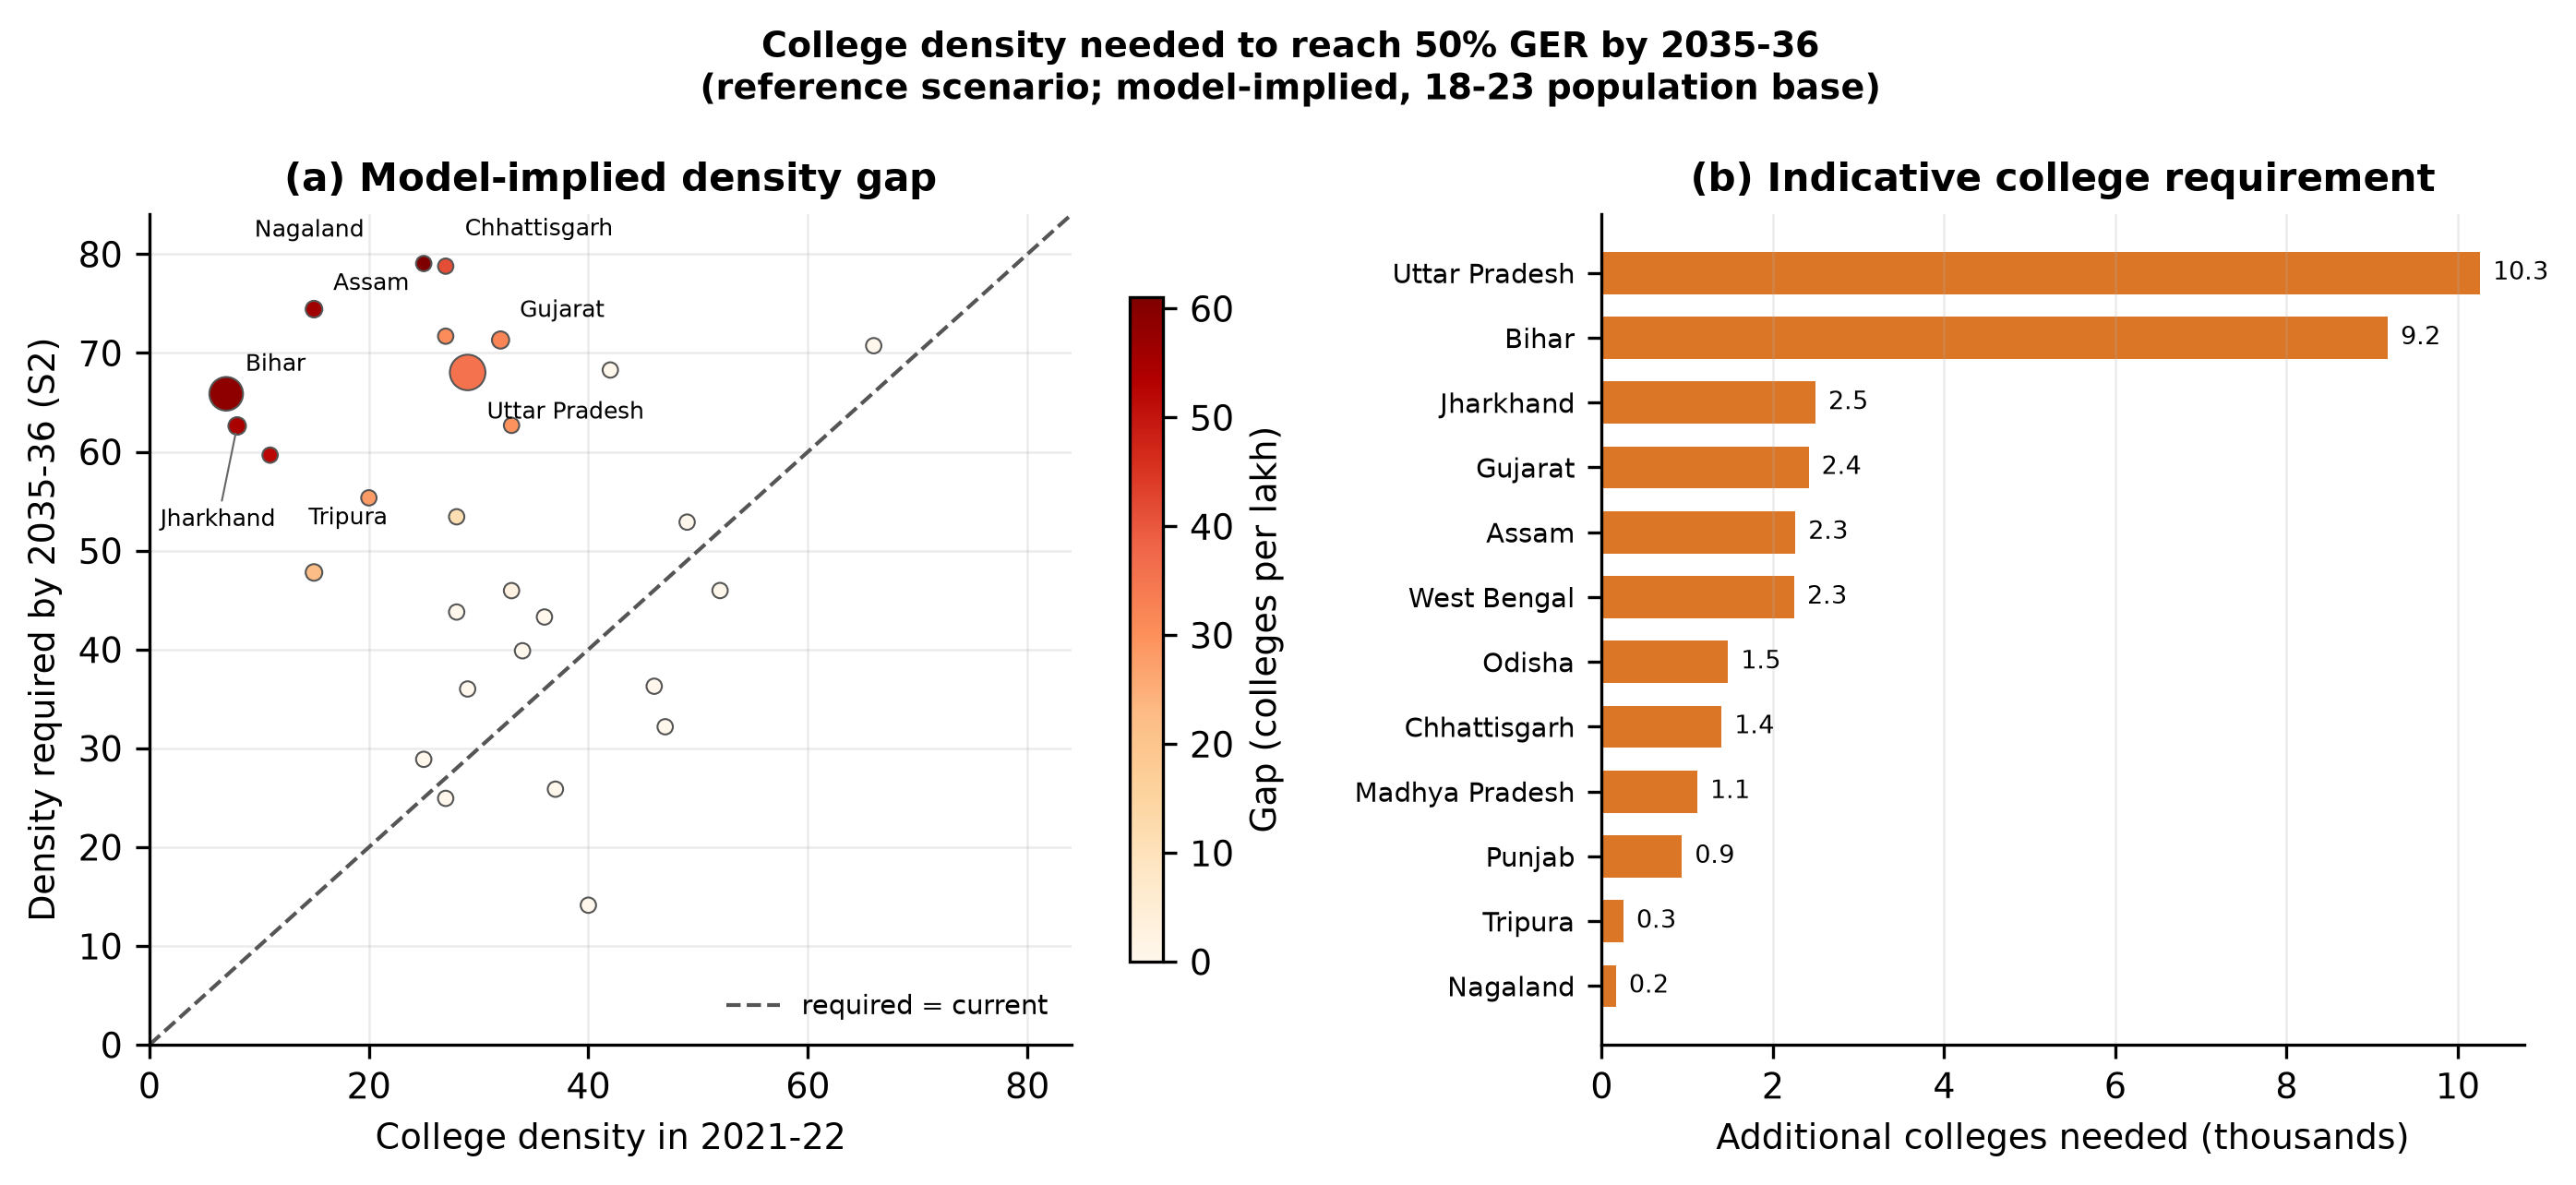
\includegraphics[width=\linewidth]{fig15_required_density.png}
\caption{Model-implied college density required to reach 50\% by 2035-36, and the indicative additional-college requirement, 28 States. Panel (a) plots current density against required density; panel (b) ranks States by the implied number of additional colleges. Source: \texttt{fig15\_required\_density.png}.}
\label{fig:required}
\end{figure}

The indicative additional-college calculation gives the largest figures for Uttar Pradesh (about 10,300), Bihar (about 9,200), Jharkhand (2,500), Gujarat (2,400), Assam (2,300), West Bengal (2,300), Odisha (1,500), Chhattisgarh (1,400) and Madhya Pradesh (1,100). Figure~\ref{fig:required} places the current and required densities side by side. These figures are illustrative. They extrapolate the linear density coefficient far beyond the observed range and ignore teacher supply, funding, land and demand. They should be read as a signal of the scale of the gap, not as a costed plan.

A cautionary comparison is useful. Karnataka already has 66 colleges per lakh, roughly the density the model says Bihar needs, but its GER is 36.2\%, not 50\%. Density is therefore necessary but not sufficient. Demand, quality, programme mix and completion also matter. The required-density figures describe the capacity gap implied by the cross-sectional association; they do not guarantee that reaching that density will deliver 50\%.

\subsection{Union Territories}

The UT appendix is indicative only, because UTs were outside the estimation sample. Applying the 28-State coefficients, Chandigarh (64.8) and Puducherry (61.5) are already above 50\%; Delhi (49.0) is projected at 61.1 with \(P = 0.95\); Jammu and Kashmir (24.8) at 34.5 with \(P = 0.01\); the Andaman and Nicobar Islands (22.6) at 39.7 with \(P = 0.08\); and Dadra and Nagar Haveli and Daman and Diu (11.2) at 17.7 with \(P \approx 0\). Ladakh and Lakshadweep are omitted because of missing predictors or an insufficient panel. The UT results should not be used for policy targeting without a separate city-catchment analysis.

\section{Discussion}\label{sec:discussion}

\subsection{Why density, and why not PTR or GPI}

The robust density association is consistent with an access story. States with more colleges per eligible population have lower travel and transaction costs, more programme choice and more competition, all of which can raise participation. The coefficient is conditional on PTR and GPI, but it may still pick up the fact that high-density States are richer or more urban. It is a cross-sectional association: States that build colleges may also be the States that invest in schools, roads and scholarships. The panel result, especially the larger first-difference coefficient, is reassuring but not decisive; a short panel cannot separate the effect of expansion from a simultaneous demand shock. The result is also consistent with the recent finding that private provision narrows regional GER gaps in India, since private colleges are concentrated where density is already high \cite{sharma2026}.

The PTR result is a cautionary tale. A negative bivariate correlation between PTR and GER is often read as evidence that teacher shortages depress enrolment. The panel shows that the sign is not stable. With State fixed effects and in first differences, the PTR coefficient becomes positive. This is consistent with reverse causality and with the mechanical definition of PTR. The appropriate conclusion is not that teachers do not matter, but that this design cannot identify their causal effect. A credible teacher-supply analysis would need instrumented or policy-induced variation in hiring, or administrative data linking teachers to institutions and programmes.

The GPI result is similarly nuanced. Ten States have GPI below 1.0, and gender gaps in higher education remain a serious equity concern \cite{ghosh2021}. But the aggregate GER is already near parity in most States, and the remaining variation is not strongly associated with the aggregate once density and PTR are controlled. Gender parity should be evaluated with female GER, field-of-study segregation and completion as outcomes, not only as a regressor for the aggregate.

\subsection{Why the national target is harder than a count of States}

The reference scenario reaches 13 of 28 States, but the population-weighted GER is only 43.5\%. The States below 50\% include Bihar, Uttar Pradesh, Madhya Pradesh, Jharkhand, Assam, West Bengal and Odisha, which together account for a large share of the 18--23 population. A national target is not a count of States; it is a population-weighted outcome. The unweighted ``13 of 28'' therefore overstates progress. This is the same aggregation problem that Kadlak and Behera~\cite{kadlak2026} identify at the district level: a State or national ratio can improve while the places with the largest youth cohorts fall further behind.

The reform scenario is instructive. PTR convergence to 20 and GPI convergence to 1.05 raise the mean projection by about 1.2 points, but they do not move any additional State across the 50\% line. In this model, the quality and parity levers are too small, and too imprecisely estimated, to close a 20-point gap. Density expansion and the secular participation trend do most of the work. This does not mean quality reforms are unimportant; it means they are unlikely to be sufficient on their own, and that a credible 2035 strategy needs a large capacity component in the low-density States.

\subsection{Policy implications}

Five implications follow, with the caveat that expansion without learning gains can leave graduates without the skills that higher education is meant to provide \cite{unesco2020}.

\begin{enumerate}
  \item \textbf{Differentiate the target by State group.} The southern and hilly States (Tamil Nadu, Kerala, Karnataka, Telangana, Himachal Pradesh, Uttarakhand, Sikkim) are broadly on track; the priority there is quality, research and graduate outcomes, not raw capacity. The low-density populous States (Bihar, Uttar Pradesh, Madhya Pradesh, Jharkhand, Assam, West Bengal, Odisha, Chhattisgarh) need a capacity push.
  \item \textbf{Measure density against the 18--23 population.} The same number of colleges implies very different access in States with different age structures. A target based on total population would understate the need in high-fertility States.
  \item \textbf{Pair expansion with teacher hiring.} Building colleges without teachers would raise PTR and dilute quality. The positive PTR coefficient in the fixed-effects models is a warning that enrolment growth can outrun teacher supply.
  \item \textbf{Do not use the aggregate GER as the only gender indicator.} GPI is near parity in most States; the remaining gaps are better studied with female GER, field segregation and completion.
  \item \textbf{Report uncertainty.} A point forecast of 50\% in 2035 is not a plan. The 5th--95th intervals span 20 points or more for many States; policy should be robust to that uncertainty, not anchored to a single number.
\end{enumerate}

\subsection{What the machine-learning comparison adds}

The model comparison is not a tournament in which the most flexible model wins. The polynomial has the best LOOCV error, but it is non-monotone outside the observed range and unsuitable for extrapolation. The tuned tree and \(k\)-NN have high in-sample \(R^2\) but poor out-of-sample error, and their nested scores expose the optimism of tuning on 28 observations. OLS is not the best predictor, but it is within about 15\% of the best RMSE, it is interpretable, and it supports the inference and projection that the policy question requires. This is a practical illustration of the distinction between prediction and explanation \cite{mullainathan2017,athey2019}.

\section{Limitations and Threats to Validity}\label{sec:limitations}

\begin{enumerate}
  \item \textbf{Cross-sectional association is not causation.} The density coefficient is conditional on PTR and GPI; it does not identify the effect of building a college. Omitted variables such as income, urbanisation, secondary completion, private provision, distance education and State capacity may drive both density and GER.
  \item \textbf{Small \(n\).} With 28 States and three predictors, the model has limited power. The GPI coefficient is essentially unidentified, and the confidence intervals for PTR and GPI are wide. LOOCV is the right protocol, but it cannot create information that the sample does not contain.
  \item \textbf{PTR endogeneity.} PTR is mechanically related to enrolment and teacher supply. Its sign flips across specifications, so it should not be read as a causal lever.
  \item \textbf{Omitted variables.} The model explains about 54\% of cross-State variance in-sample and 37\% out-of-sample. The residual pattern (Tamil Nadu under-predicted, Karnataka over-predicted) shows that the three indicators do not capture demand, quality or private provision.
  \item \textbf{Extrapolation.} The projection applies a linear density coefficient far beyond the observed range (maximum 66) and caps density at 100. The required-density and additional-college figures are model-implied illustrations, not costed plans.
  \item \textbf{Trend assumption.} The 0.866-point annual trend is an average from a short, Covid-affected panel. It may not continue for 14 years, and it is unlikely to be the same in every State.
  \item \textbf{UT exclusion.} UTs are excluded from estimation for methodological reasons; their appendix projections are indicative only.
  \item \textbf{Data revisions and reporting breaks.} GER 2021-22 is provisional in the OGD release; AISHE figures may be revised. The 2011 Census population projection is the denominator for both GER and density. Reporting practice can also break a series abruptly, as Sikkim's 2019-20 value illustrates; such breaks are annotated and tested rather than smoothed away.
  \item \textbf{No spatial dependence.} Neighbouring States may share students, teachers and labour markets; the model treats them as independent.
  \item \textbf{No policy cost.} The analysis does not estimate the fiscal cost of expansion, the supply of qualified teachers, or the demand response to new colleges.
  \item \textbf{Single post-Covid cross-section.} The estimation sample is one year. A second year of AISHE data, or a district-level check for a few States, would allow the density association to be tested against a different population and reporting regime, and would make the paper more competitive for a journal submission.
\end{enumerate}

\section{Conclusion and Future Work}\label{sec:conclusion}

The 50\% GER target is achievable for about half of the States under a continuation of recent trends, but not for the States that account for most of India's young population. College density is the most robust correlate of GER and the lever with the largest projected effect. PTR and GPI are important for quality and equity, but they do not carry independent explanatory power for the aggregate in this cross-section. The population-weighted GER is projected at 43.5\% in 2035-36 under the reference scenario, 6.5 points short of the target, with 68.6\% of the 18--23 population in States below 50\%.

The policy message is twofold. First, the target is off track in the populous low-density States, and a national strategy that focuses on the already-high-GER States will not deliver it. Second, capacity expansion must be paired with teacher supply and equity policies, because the quality and parity levers in this model are too weak to close the gap on their own. A credible 2035 strategy needs a differentiated, State-specific mix of expansion, quality and equity, monitored with uncertainty rather than a single point forecast.

Future work should extend the panel beyond 2021-22, add a second year of AISHE data or a district-level check for a few States, and use institution-level data to reduce aggregation bias. It should also test whether the density association survives a credible identification strategy such as a policy-induced expansion programme, and model female GER and field-of-study segregation directly rather than treating gender parity as a regressor for the aggregate.

\begin{credits}

\subsubsection{\ackname}
The author thanks the Department of Computer Science, Ramanujan College, University of Delhi, and course supervisor Nikhil Sir for constructive feedback on the initial manuscript.

\subsubsection{\discintname}
The author declares no competing interests to declare that are relevant to the content of this article.

\subsubsection{Data and code availability.}
The target is the Open Government Data Platform India resource \emph{States/UT-wise Gross Enrolment Ratio (GER) in Higher Education Based on 2011 Population Census Projection for 18--23 Age Group during 2021-22}, resource ID \texttt{7edbaeed-65e9-43ad-8f81-730187b70463}. The resource is released under the Government Open Data Licence--India (GODL-India) and was retrieved on 25 October 2026 from \url{https://www.data.gov.in/resource/statesut-wise-gross-enrolment-ratio-ger-higher-education-based-2011-population-census}. The predictors are from the AISHE 2021-22 Final Report \cite{aishe2023}. The raw files, retrieval metadata, SHA-256 checksums, processed analysis files, validation log (\path{data/processed/extraction_validation.txt}) and full pipeline (\path{src/run_all.py}, \path{src/verify_outputs.py}) are available at \url{https://github.com/Himanshu2ht/Modelling-Gross-Enrolment-Ratio-GER-in-Higher-Education-Across-States}.

\subsubsection{Ethics and funding.}
The data are aggregate administrative statistics with no personal information. The main ethical risk is over-reliance on a forecast: a missed target or a misallocated college budget can affect access for vulnerable groups, so uncertainty intervals and limitations should be read alongside point estimates. This research received no external funding.

\subsubsection{Use of AI tools.}
AI assistants (DeepSeek V4.1 Flash via OpenCode for the initial LaTeX conversion and \path{src/checks.py}; Gemini via Antigravity CLI for the Springer LNCS template conversion, workflow diagram, notation alignment, abstract tightening, updating \path{src/run_all.py} and \path{src/verify_outputs.py}, and pinning \path{requirements.txt}) were used to (i) draft and edit prose in the Introduction, Related Work, Discussion and Limitations; (ii) format the LaTeX tables, equations and bibliography; and (iii) refactor parts of \path{src/modeling.py} and \path{src/projection.py} and integrate \path{src/checks.py}. All data extraction and model estimation were executed locally from \path{src/}, every DOI was verified against Crossref, and every number in the article is reproduced by \path{src/run_all.py} and checked by \path{src/verify_outputs.py}. The author reviewed all text and code and takes full responsibility for the final submission.

\end{credits}


\bibliographystyle{splncs04}
\bibliography{references}

\appendix
\section{Per-State Results}

Table~\ref{tab:appendix} reports the full per-State detail: observed GER, leave-one-out prediction from the OLS three-indicator model, projected GER in 2035-36 under S2, the 5th and 95th percentile bootstrap bounds, the probability of reaching 50\%, and the resulting status.

\begin{sidewaystable}[p]
\centering
\caption{Per-State results, 28 States. LOOCV predictions are from the OLS three-indicator model; projections are from S2 with 2,000 bootstrap draws. Status follows the rule in Section~\ref{sec:projection}: On track if \(P(\GER \ge 50\%) \ge 0.5\), At risk if \(0.15 \le P < 0.5\), Off track otherwise. Source: \texttt{table11\_state\_appendix.csv}.}
\label{tab:appendix}
\resizebox{\textwidth}{!}{%
\begin{tabular}{@{}lrrrrrrrrrl@{}}
\toprule
State & GER 2021 & LOOCV prediction & LOOCV error & Density 2021 & Density 2035 & GER 2035 (S2) & 5th pct & 95th pct & \(P(\GER \ge 50\%)\) & Status \\
\midrule
Tamil Nadu & 47.0 & 34.5 & +12.5 & 40 & 57.5 & 65.3 & 53.7 & 77.4 & 0.98 & On track \\
Himachal Pradesh & 43.1 & 33.9 & +9.2 & 47 & 54.0 & 57.7 & 46.2 & 68.5 & 0.88 & On track \\
Uttarakhand & 41.8 & 32.6 & +9.2 & 37 & 37.0 & 53.9 & 42.9 & 65.3 & 0.73 & On track \\
Kerala & 41.3 & 36.2 & +5.1 & 46 & 53.0 & 55.9 & 44.7 & 67.3 & 0.81 & On track \\
Telangana & 40.0 & 39.4 & +0.6 & 52 & 55.5 & 53.4 & 41.8 & 64.2 & 0.68 & On track \\
Sikkim & 38.6 & 29.5 & +9.1 & 27 & 44.5 & 56.9 & 45.6 & 69.4 & 0.85 & On track \\
Andhra Pradesh & 36.5 & 38.6 & $-2.1$ & 49 & 52.5 & 49.9 & 38.8 & 61.0 & 0.49 & At risk \\
Arunachal Pradesh & 36.5 & 27.5 & +9.0 & 25 & 46.0 & 56.0 & 44.7 & 68.9 & 0.80 & On track \\
Karnataka & 36.2 & 48.8 & $-12.6$ & 66 & 100.0 & 60.3 & 46.9 & 75.1 & 0.90 & On track \\
Goa & 35.8 & 33.0 & +2.8 & 34 & 41.0 & 50.4 & 39.3 & 61.7 & 0.53 & On track \\
Manipur & 35.4 & 30.4 & +5.0 & 29 & 39.5 & 51.2 & 40.3 & 62.8 & 0.58 & On track \\
Maharashtra & 35.3 & 32.1 & +3.2 & 36 & 46.5 & 51.1 & 40.0 & 62.5 & 0.57 & On track \\
Haryana & 33.3 & 31.6 & +1.7 & 33 & 43.5 & 49.1 & 37.6 & 60.5 & 0.47 & At risk \\
Mizoram & 32.3 & 30.7 & +1.6 & 28 & 45.5 & 50.6 & 38.6 & 63.0 & 0.53 & On track \\
Madhya Pradesh & 28.9 & 28.2 & +0.7 & 28 & 42.0 & 46.0 & 34.6 & 57.5 & 0.29 & At risk \\
Rajasthan & 28.6 & 34.6 & $-6.0$ & 42 & 73.5 & 51.8 & 38.6 & 65.4 & 0.60 & On track \\
Punjab & 27.4 & 33.5 & $-6.1$ & 33 & 33.0 & 39.5 & 28.4 & 51.1 & 0.07 & Off track \\
West Bengal & 26.3 & 23.7 & +2.6 & 15 & 25.5 & 42.1 & 30.7 & 53.9 & 0.15 & Off track \\
Meghalaya & 25.4 & 27.4 & $-2.0$ & 20 & 27.0 & 40.0 & 28.4 & 51.7 & 0.07 & Off track \\
Uttar Pradesh & 24.1 & 28.0 & $-3.9$ & 29 & 32.5 & 37.5 & 26.3 & 48.9 & 0.03 & Off track \\
Gujarat & 24.0 & 30.8 & $-6.8$ & 32 & 39.0 & 38.6 & 27.9 & 50.4 & 0.05 & Off track \\
Odisha & 22.1 & 30.1 & $-8.0$ & 27 & 41.0 & 39.2 & 27.8 & 51.6 & 0.07 & Off track \\
Tripura & 20.7 & 21.2 & $-0.5$ & 11 & 7.5 & 31.6 & 19.9 & 42.6 & 0.00 & Off track \\
Chhattisgarh & 19.6 & 29.8 & $-10.2$ & 27 & 37.5 & 35.4 & 23.9 & 47.0 & 0.01 & Off track \\
Nagaland & 18.8 & 31.6 & $-12.8$ & 25 & 18.0 & 28.5 & 17.1 & 39.6 & 0.00 & Off track \\
Jharkhand & 18.6 & 15.9 & +2.7 & 8 & 8.0 & 30.7 & 19.5 & 41.9 & 0.00 & Off track \\
Bihar & 17.1 & 11.8 & +5.3 & 7 & 7.0 & 29.2 & 17.9 & 40.9 & 0.00 & Off track \\
Assam & 16.9 & 25.8 & $-8.9$ & 15 & 18.5 & 30.3 & 18.9 & 41.4 & 0.00 & Off track \\
\bottomrule
\end{tabular}}
\end{sidewaystable}

\section{Reproduction Checklist}

\begin{enumerate}
  \item \path{python src/download_data.py} --- downloads the OGD JSON and the AISHE PDF and writes SHA-256 checksums.
  \item \path{python src/extract_aishe.py} --- extracts AISHE Tables 4, 42, 47, 48 and 49 and writes \path{extraction_validation.txt}.
  \item \path{python src/build_dataset.py} --- merges the OGD target with the AISHE predictors and derives the analysis variables.
  \item \path{python src/eda.py} --- writes Tables~\ref{tab:descriptives}--\ref{tab:correlations} and Figures~\ref{fig:ranked}--\ref{fig:trajectories}.
  \item \path{python src/checks.py} --- writes the missingness and log-transform tables (Tables~\ref{tab:missing} and~\ref{tab:log}; files \path{table13_missingness.csv}, \path{table12_log_transform.csv} and \path{table12b_skewness.csv}).
  \item \path{python src/modeling.py} --- writes the model comparison, coefficients, diagnostics, sensitivity table, hyper-parameter table and Figures~\ref{fig:modelcomp}--\ref{fig:poly}.
  \item \path{python src/projection.py} --- writes the projections, required density, scenario summary, per-State appendix and Figures~\ref{fig:dumbbell}--\ref{fig:required}.
  \item \path{python src/verify_outputs.py} --- checks the headline numbers against the stored outputs.
  \item \path{cd paper && tectonic paper.tex} --- builds \path{paper.pdf} from the Springer LNCS LaTeX source (with \path{llncs.cls} and \path{splncs04.bst} bundled for Overleaf and standard TeX installations).
\end{enumerate}

All steps are deterministic given the raw files and \texttt{RANDOM\_STATE = 42}. The pipeline can be run end to end with \texttt{python src/run\_all.py} (or \texttt{./run.sh} on Linux).


\end{document}
